% Cursus Onderzoekstechnieken
\documentclass[11pt,fleqn,a4paper]{book}

%%%%%%%%%%%%%%%%%%%%%%%%%%%%%%%%%%%%%%%%%
% The Legrand Orange Book
% Structural Definitions File
% Version 2.0 (9/2/15)
%
% Original author:
% Mathias Legrand (legrand.mathias@gmail.com) with modifications by:
% Vel (vel@latextemplates.com)
%
% This file has been downloaded from:
% http://www.LaTeXTemplates.com
%
% License:
% CC BY-NC-SA 3.0 (http://creativecommons.org/licenses/by-nc-sa/3.0/)
%
%%%%%%%%%%%%%%%%%%%%%%%%%%%%%%%%%%%%%%%%%

%----------------------------------------------------------------------------------------
%	VARIOUS REQUIRED PACKAGES AND CONFIGURATIONS
%----------------------------------------------------------------------------------------

\usepackage[top=3cm,bottom=3cm,left=3cm,right=3cm,headsep=10pt,a4paper]{geometry} % Page margins
\usepackage[margin=1cm,labelfont=bf]{caption}
\usepackage{graphicx} % Required for including pictures
\graphicspath{{images/}} % Specifies the directory where pictures are stored

\usepackage{titling} % Macros for title, author, etc

\usepackage[toc,page]{appendix}
\usepackage{tikz} % Required for drawing custom shapes
\usepackage{pgfplotstable}
\usepackage{pgfplots}
\pgfplotsset{compat=1.13}
\usetikzlibrary{arrows,shapes,backgrounds,positioning,shadows}
\usetikzlibrary{pgfplots.statistics}

\usepackage[english,dutch]{babel} % English language/hyphenation
\usepackage{iflang}

\usepackage{paralist}
\usepackage{enumitem} % Customize lists
\setlist{nolistsep} % Reduce spacing between bullet points and numbered lists

\usepackage{booktabs} % Required for nicer horizontal rules in tables
\usepackage{subcaption}
\usepackage{multirow}

\usepackage{xcolor} % Required for specifying colors by name
\definecolor{maincolor}{RGB}{0,100,184} % Define the main color used for highlighting throughout the book
\definecolor{hogentblue}{RGB}{0,111,184} % Define the orange color used for highlighting throughout the book

% Paragraph style: no indent, add space between paragraphs
\setlength{\parindent}{0em}
\setlength{\parskip}{1em}

\usepackage{comment} % Gebruikt om oplossingen al dan niet mee te nemen in het compileren

%----------------------------------------------------------------------------------------
%	FONTS
%----------------------------------------------------------------------------------------

\usepackage{avant} % Use the Avantgarde font for headings
%\usepackage{times} % Use the Times font for headings
\usepackage{mathptmx} % Use the Adobe Times Roman as the default text font together with math symbols from the Sym­bol, Chancery and Com­puter Modern fonts
\usepackage{eurosym}

\usepackage{amsfonts}
\usepackage{amsmath}
\usepackage{amssymb}
\usepackage{textcomp}
\usepackage{wasysym}

\usepackage{microtype} % Slightly tweak font spacing for aesthetics
\usepackage[utf8]{inputenc} % Required for including letters with accents
\usepackage[T1]{fontenc} % Use 8-bit encoding that has 256 glyphs

%%============================================================================
%% Colours HoGent corporate identity
%%============================================================================

% Faculty colours
\definecolor{HoGentFBO}{RGB}{0,147,208} % Bedrijf en Organisatie
\definecolor{HoGentFMW}{RGB}{0,168,143} % Mens en Wetenschappen
\definecolor{HoGentFNT}{RGB}{255,0,0}   % Natuur en Techniek
\definecolor{HoGentSoA}{RGB}{0,0,0}     % School of Arts

% Accent colours
\definecolor{HoGentAccent1}{RGB}{0,111,184}   % Dark blue
\definecolor{HoGentAccent2}{RGB}{244,52,69}   % Red
\definecolor{HoGentAccent3}{RGB}{0,156,124}   % Green
\definecolor{HoGentAccent4}{RGB}{239,170,162} % Pink
\definecolor{HoGentAccent5}{RGB}{150,150,150} % Grey
\definecolor{HoGentAccent6}{RGB}{255,218,0}   % Yellow

% Aliases for accent colours
\colorlet{HoGentBlue}{HoGentAccent1}
\colorlet{HoGentRed}{HoGentAccent2}
\colorlet{HoGentGreen}{HoGentAccent3}
\colorlet{HoGentPink}{HoGentAccent4}
\colorlet{HoGentGrey}{HoGentAccent5}
\colorlet{HoGentYellow}{HoGentAccent6}

%------------------------------------------------------------------------------
%	TITLE PAGE
%------------------------------------------------------------------------------

\newcommand{\thetitlepage}{%
\begingroup
\thispagestyle{empty}
\begin{tikzpicture}[remember picture,overlay]
\coordinate [below=12cm] (midpoint) at (current page.north);
\node at (current page.north west)
{\begin{tikzpicture}[remember picture,overlay]
\node[anchor=north west,inner sep=0pt] at (0,0) {
\includegraphics[width=\paperwidth]{background.pdf}}; % Background image
\draw[anchor=north] (midpoint) node [fill=maincolor,fill opacity=0,text=white,text opacity=1,inner sep=1cm]{\Huge\centering\bfseries\sffamily\parbox[c][][t]{\paperwidth}{\centering \thetitle\\[15pt] % Book title
{\Large \thedate}\\[20pt] % Subtitle
{\large \theauthor}}}; % Author name
\end{tikzpicture}};
\end{tikzpicture}
\vfill
\endgroup
}

%----------------------------------------------------------------------------------------
%	BIBLIOGRAPHY AND INDEX
%----------------------------------------------------------------------------------------

\usepackage[style=apa,backend=biber]{biblatex}
\usepackage{csquotes}
\DeclareLanguageMapping{dutch}{dutch-apa}
\addbibresource{biblio.bib} % BibTeX bibliography file
\defbibheading{bibempty}{}

\usepackage{calc} % For simpler calculation - used for spacing the index letter headings correctly
\usepackage{makeidx} % Required to make an index
\makeindex % Tells LaTeX to create the files required for indexing

%----------------------------------------------------------------------------------------
%	MAIN TABLE OF CONTENTS
%----------------------------------------------------------------------------------------

\usepackage{titletoc} % Required for manipulating the table of contents

\contentsmargin{0cm} % Removes the default margin

% Part text styling
\titlecontents{part}[0cm]
{\addvspace{20pt}\centering\large\bfseries}
{}
{}
{}

% Chapter text styling
\titlecontents{chapter}[1.25cm] % Indentation
{\addvspace{12pt}\large\sffamily\bfseries} % Spacing and font options for chapters
{\color{maincolor!60}\contentslabel[\Large\thecontentslabel]{1.25cm}\color{maincolor}} % Chapter number
{\color{maincolor}}
{\color{maincolor!60}\normalsize\;\titlerule*[.5pc]{.}\;\thecontentspage} % Page number

% Section text styling
\titlecontents{section}[1.25cm] % Indentation
{\addvspace{3pt}\sffamily\bfseries} % Spacing and font options for sections
{\contentslabel[\thecontentslabel]{1.25cm}} % Section number
{}
{\hfill\color{black}\thecontentspage} % Page number
[]

% Subsection text styling
\titlecontents{subsection}[1.25cm] % Indentation
{\addvspace{1pt}\sffamily\small} % Spacing and font options for subsections
{\contentslabel[\thecontentslabel]{1.25cm}} % Subsection number
{}
{\ \titlerule*[.5pc]{.}\;\thecontentspage} % Page number
[]

% List of figures
\titlecontents{figure}[0em]
{\addvspace{-5pt}\sffamily}
{\thecontentslabel\hspace*{1em}}
{}
{\ \titlerule*[.5pc]{.}\;\thecontentspage}
[]

% List of tables
\titlecontents{table}[0em]
{\addvspace{-5pt}\sffamily}
{\thecontentslabel\hspace*{1em}}
{}
{\ \titlerule*[.5pc]{.}\;\thecontentspage}
[]

%----------------------------------------------------------------------------------------
%	MINI TABLE OF CONTENTS IN PART HEADS
%----------------------------------------------------------------------------------------

% Chapter text styling
\titlecontents{lchapter}[0em] % Indenting
{\addvspace{15pt}\large\sffamily\bfseries} % Spacing and font options for chapters
{\color{maincolor}\contentslabel[\Large\thecontentslabel]{1.25cm}\color{maincolor}} % Chapter number
{}
{\color{maincolor}\normalsize\sffamily\bfseries\;\titlerule*[.5pc]{.}\;\thecontentspage} % Page number

% Section text styling
\titlecontents{lsection}[0em] % Indenting
{\sffamily\small} % Spacing and font options for sections
{\contentslabel[\thecontentslabel]{1.25cm}} % Section number
{}
{}

% Subsection text styling
\titlecontents{lsubsection}[.5em] % Indentation
{\normalfont\footnotesize\sffamily} % Font settings
{}
{}
{}

%----------------------------------------------------------------------------------------
%	PAGE HEADERS
%----------------------------------------------------------------------------------------

\usepackage{fancyhdr} % Required for header and footer configuration

\pagestyle{fancy}
\renewcommand{\chaptermark}[1]{\markboth{\sffamily\normalsize\bfseries\chaptername\ \thechapter.\ #1}{}} % Chapter text font settings
\renewcommand{\sectionmark}[1]{\markright{\sffamily\normalsize\thesection\hspace{5pt}#1}{}} % Section text font settings
\fancyhf{} \fancyhead[LE,RO]{\sffamily\normalsize\thepage} % Font setting for the page number in the header
\fancyhead[LO]{\rightmark} % Print the nearest section name on the left side of odd pages
\fancyhead[RE]{\leftmark} % Print the current chapter name on the right side of even pages
\renewcommand{\headrulewidth}{0.5pt} % Width of the rule under the header
\addtolength{\headheight}{2.5pt} % Increase the spacing around the header slightly
\renewcommand{\footrulewidth}{0pt} % Removes the rule in the footer
\fancypagestyle{plain}{\fancyhead{}\renewcommand{\headrulewidth}{0pt}} % Style for when a plain pagestyle is specified

% Removes the header from odd empty pages at the end of chapters
\makeatletter
\renewcommand{\cleardoublepage}{
\clearpage\ifodd\c@page\else
\hbox{}
\vspace*{\fill}
\thispagestyle{empty}
\newpage
\fi}

%----------------------------------------------------------------------------------------
%	THEOREM STYLES
%----------------------------------------------------------------------------------------

\usepackage{amsmath,amsfonts,amssymb,amsthm} % For math equations, theorems, symbols, etc

\newcommand{\intoo}[2]{\mathopen{]}#1\,;#2\mathclose{[}}
\newcommand{\ud}{\mathop{\mathrm{{}d}}\mathopen{}}
\newcommand{\intff}[2]{\mathopen{[}#1\,;#2\mathclose{]}}
\newtheorem{notation}{Notation}[chapter]

% Boxed/framed environments
\newtheoremstyle{maincolornumbox}% % Theorem style name
{0pt}% Space above
{0pt}% Space below
{\normalfont}% % Body font
{}% Indent amount
{\small\bf\sffamily\color{maincolor}}% % Theorem head font
{\;}% Punctuation after theorem head
{0.25em}% Space after theorem head
{\small\sffamily\color{maincolor}\thmname{#1}\nobreakspace\thmnumber{\@ifnotempty{#1}{}\@upn{#2}}% Theorem text (e.g. Theorem 2.1)
\thmnote{\nobreakspace\the\thm@notefont\sffamily\bfseries\color{black}---\nobreakspace#3.}} % Optional theorem note
\renewcommand{\qedsymbol}{$\blacksquare$}% Optional qed square

\newtheoremstyle{blacknumex}% Theorem style name
{5pt}% Space above
{5pt}% Space below
{\normalfont}% Body font
{} % Indent amount
{\small\bf\sffamily}% Theorem head font
{\;}% Punctuation after theorem head
{0.25em}% Space after theorem head
{\small\sffamily{\tiny\ensuremath{\blacksquare}}\nobreakspace\thmname{#1}\nobreakspace\thmnumber{\@ifnotempty{#1}{}\@upn{#2}}% Theorem text (e.g. Theorem 2.1)
\thmnote{\nobreakspace\the\thm@notefont\sffamily\bfseries---\nobreakspace#3.}}% Optional theorem note

\newtheoremstyle{blacknumbox} % Theorem style name
{0pt}% Space above
{0pt}% Space below
{\normalfont}% Body font
{}% Indent amount
{\small\bf\sffamily}% Theorem head font
{\;}% Punctuation after theorem head
{0.25em}% Space after theorem head
{\small\sffamily\thmname{#1}\nobreakspace\thmnumber{\@ifnotempty{#1}{}\@upn{#2}}% Theorem text (e.g. Theorem 2.1)
\thmnote{\nobreakspace\the\thm@notefont\sffamily\bfseries---\nobreakspace#3.}}% Optional theorem note

% Non-boxed/non-framed environments
\newtheoremstyle{maincolornum}% % Theorem style name
{5pt}% Space above
{5pt}% Space below
{\normalfont}% % Body font
{}% Indent amount
{\small\bf\sffamily\color{maincolor}}% % Theorem head font
{\;}% Punctuation after theorem head
{0.25em}% Space after theorem head
{\small\sffamily\color{maincolor}\thmname{#1}\nobreakspace\thmnumber{\@ifnotempty{#1}{}\@upn{#2}}% Theorem text (e.g. Theorem 2.1)
\thmnote{\nobreakspace\the\thm@notefont\sffamily\bfseries\color{black}---\nobreakspace#3.}} % Optional theorem note
\renewcommand{\qedsymbol}{$\blacksquare$}% Optional qed square
\makeatother

%----------------------------------------------------------------------------------------
%	DEFINITION OF COLORED BOXES
%----------------------------------------------------------------------------------------

\RequirePackage[framemethod=default]{mdframed} % Required for creating the theorem, definition, exercise and corollary boxes

\newcounter{dummy} 
\newtheorem{theoremeT}[dummy]{Stelling}
\newtheorem{problem}{Probleem}[chapter]
\newtheorem{exerciseT}{Oefening}[chapter]
\newtheorem{exampleT}{Voorbeeld}[chapter]
\newtheorem{definitionT}{Definitie}[section]

% Theorem box
\newmdenv[skipabove=7pt,
skipbelow=7pt,
backgroundcolor=black!5,
linecolor=maincolor,
innerleftmargin=5pt,
innerrightmargin=5pt,
innertopmargin=7pt,
innerbottommargin=7pt,
leftmargin=0cm,
rightmargin=0cm,
innerbottommargin=5pt]{tBox}

% Exercise box
\newmdenv[skipabove=7pt,
skipbelow=7pt,
rightline=false,
leftline=true,
topline=false,
bottomline=false,
backgroundcolor=maincolor!10,
linecolor=maincolor,
innerleftmargin=5pt,
innerrightmargin=5pt,
innertopmargin=7pt,
innerbottommargin=7pt,
leftmargin=0cm,
rightmargin=0cm,
linewidth=4pt]{eBox}

% Definition box
\newmdenv[skipabove=7pt,
skipbelow=7pt,
rightline=false,
leftline=true,
topline=false,
bottomline=false,
linecolor=maincolor,
innerleftmargin=5pt,
innerrightmargin=5pt,
innertopmargin=7pt,
innerbottommargin=7pt,
leftmargin=0cm,
rightmargin=0cm,
linewidth=4pt,
innerbottommargin=0pt]{dBox}

% Corollary box
\newmdenv[skipabove=7pt,
skipbelow=7pt,
rightline=false,
leftline=true,
topline=false,
bottomline=false,
linecolor=gray,
backgroundcolor=black!5,
innerleftmargin=5pt,
innerrightmargin=5pt,
innertopmargin=7pt,
innerbottommargin=7pt,
leftmargin=0cm,
rightmargin=0cm,
linewidth=4pt,
innerbottommargin=5pt]{cBox}

% Creates an environment for each type of theorem and assigns it a theorem text style from the "Theorem Styles" section above and a colored box from above
\newenvironment{theorem}{\begin{tBox}\begin{theoremeT}}{\end{theoremeT}\end{tBox}}
\newenvironment{exercise}{\begin{eBox}\begin{exerciseT}}{\hfill{\color{maincolor}\tiny\ensuremath{\blacksquare}}\end{exerciseT}\end{eBox}}
\newenvironment{definition}{\begin{dBox}\begin{definitionT}}{\end{definitionT}\end{dBox}}
\newenvironment{example}{\begin{exampleT}}{\hfill{\tiny\ensuremath{\blacksquare}}\end{exampleT}}
\newenvironment{corollary}{\begin{cBox}\begin{corollaryT}}{\end{corollaryT}\end{cBox}}

%----------------------------------------------------------------------------------------
%	REMARK ENVIRONMENT
%----------------------------------------------------------------------------------------

\newenvironment{remark}{\par\vspace{10pt}\small % Vertical white space above the remark and smaller font size
\begin{list}{}{
\leftmargin=35pt % Indentation on the left
\rightmargin=25pt}\item\ignorespaces % Indentation on the right
\makebox[-2.5pt]{\begin{tikzpicture}[overlay]
\node[draw=maincolor!60,line width=1pt,circle,fill=maincolor!25,font=\sffamily\bfseries,inner sep=2pt,outer sep=0pt] at (-15pt,0pt){\textcolor{maincolor}{R}};\end{tikzpicture}} % Orange R in a circle
\advance\baselineskip -1pt}{\end{list}\vskip5pt} % Tighter line spacing and white space after remark

%----------------------------------------------------------------------------------------
%	SECTION NUMBERING IN THE MARGIN
%----------------------------------------------------------------------------------------

\makeatletter
\renewcommand{\@seccntformat}[1]{\llap{\textcolor{maincolor}{\csname the#1\endcsname}\hspace{1em}}}
\renewcommand{\section}{\@startsection{section}{1}{\z@}
{-4ex \@plus -1ex \@minus -.4ex}
{1ex \@plus.2ex }
{\normalfont\large\sffamily\bfseries}}
\renewcommand{\subsection}{\@startsection {subsection}{2}{\z@}
{-3ex \@plus -0.1ex \@minus -.4ex}
{0.5ex \@plus.2ex }
{\normalfont\sffamily\bfseries}}
\renewcommand{\subsubsection}{\@startsection {subsubsection}{3}{\z@}
{-2ex \@plus -0.1ex \@minus -.2ex}
{.2ex \@plus.2ex }
{\normalfont\small\sffamily\bfseries}}
\renewcommand\paragraph{\@startsection{paragraph}{4}{\z@}
{-2ex \@plus-.2ex \@minus .2ex}
{.1ex}
{\normalfont\small\sffamily\bfseries}}

%----------------------------------------------------------------------------------------
%	PART HEADINGS
%----------------------------------------------------------------------------------------

% numbered part in the table of contents
\newcommand{\@mypartnumtocformat}[2]{%
\setlength\fboxsep{0pt}%
\noindent\colorbox{maincolor!20}{\strut\parbox[c][.7cm]{\ecart}{\color{maincolor!70}\Large\sffamily\bfseries\centering#1}}\hskip\esp\colorbox{maincolor!40}{\strut\parbox[c][.7cm]{\linewidth-\ecart-\esp}{\Large\sffamily\centering#2}}}%
%%%%%%%%%%%%%%%%%%%%%%%%%%%%%%%%%%
% unnumbered part in the table of contents
\newcommand{\@myparttocformat}[1]{%
\setlength\fboxsep{0pt}%
\noindent\colorbox{maincolor!40}{\strut\parbox[c][.7cm]{\linewidth}{\Large\sffamily\centering#1}}}%
%%%%%%%%%%%%%%%%%%%%%%%%%%%%%%%%%%
\newlength\esp
\setlength\esp{4pt}
\newlength\ecart
\setlength\ecart{1.2cm-\esp}
\newcommand{\thepartimage}{}%
\newcommand{\partimage}[1]{\renewcommand{\thepartimage}{#1}}%
\def\@part[#1]#2{%
\ifnum \c@secnumdepth >-2\relax%
\refstepcounter{part}%
\addcontentsline{toc}{part}{\texorpdfstring{\protect\@mypartnumtocformat{\thepart}{#1}}{\partname~\thepart\ ---\ #1}}
\else%
\addcontentsline{toc}{part}{\texorpdfstring{\protect\@myparttocformat{#1}}{#1}}%
\fi%
\startcontents%
\markboth{}{}%
{\thispagestyle{empty}%
\begin{tikzpicture}[remember picture,overlay]%
\node at (current page.north west){\begin{tikzpicture}[remember picture,overlay]%
\fill[maincolor!20](0cm,0cm) rectangle (\paperwidth,-\paperheight);
\node[anchor=north] at (4cm,-3.25cm){\color{maincolor!40}\fontsize{220}{100}\sffamily\bfseries\@Roman\c@part};
\node[anchor=south east] at (\paperwidth-1cm,-\paperheight+1cm){\parbox[t][][t]{8.5cm}{
\printcontents{l}{0}{\setcounter{tocdepth}{1}}%
}};
\node[anchor=north east] at (\paperwidth-1.5cm,-3.25cm){\parbox[t][][t]{15cm}{\strut\raggedleft\color{white}\fontsize{30}{30}\sffamily\bfseries#2}};
\end{tikzpicture}};
\end{tikzpicture}}%
\@endpart}
\def\@spart#1{%
\startcontents%
\phantomsection
{\thispagestyle{empty}%
\begin{tikzpicture}[remember picture,overlay]%
\node at (current page.north west){\begin{tikzpicture}[remember picture,overlay]%
\fill[maincolor!20](0cm,0cm) rectangle (\paperwidth,-\paperheight);
\node[anchor=north east] at (\paperwidth-1.5cm,-3.25cm){\parbox[t][][t]{15cm}{\strut\raggedleft\color{white}\fontsize{30}{30}\sffamily\bfseries#1}};
\end{tikzpicture}};
\end{tikzpicture}}
\addcontentsline{toc}{part}{\texorpdfstring{%
\setlength\fboxsep{0pt}%
\noindent\protect\colorbox{maincolor!40}{\strut\protect\parbox[c][.7cm]{\linewidth}{\Large\sffamily\protect\centering #1\quad\mbox{}}}}{#1}}%
\@endpart}
\def\@endpart{\vfil\newpage
\if@twoside
\if@openright
\null
\thispagestyle{empty}%
\newpage
\fi
\fi
\if@tempswa
\twocolumn
\fi}

%----------------------------------------------------------------------------------------
%	CHAPTER HEADINGS
%----------------------------------------------------------------------------------------

% A switch to conditionally include a picture, implemented by  Christian Hupfer
\newif\ifusechapterimage
\usechapterimagetrue
\newcommand{\thechapterimage}{}%
\newcommand{\chapterimage}[1]{\ifusechapterimage\renewcommand{\thechapterimage}{#1}\fi}%
\def\@makechapterhead#1{%
{\parindent \z@ \raggedright \normalfont
\ifnum \c@secnumdepth >\m@ne
\if@mainmatter
\begin{tikzpicture}[remember picture,overlay]
\node at (current page.north west)
{\begin{tikzpicture}[remember picture,overlay]
\node[anchor=north west,inner sep=0pt] at (0,0) {\ifusechapterimage\includegraphics[width=\paperwidth]{\thechapterimage}\fi};
\draw[anchor=west] (\Gm@lmargin,-9cm) node [line width=2pt,rounded corners=15pt,draw=maincolor,fill=white,fill opacity=0.5,inner sep=15pt]{\strut\makebox[22cm]{}};
\draw[anchor=west] (\Gm@lmargin+.3cm,-9cm) node {\huge\sffamily\bfseries\color{black}\thechapter. #1\strut};
\end{tikzpicture}};
\end{tikzpicture}
\else
\begin{tikzpicture}[remember picture,overlay]
\node at (current page.north west)
{\begin{tikzpicture}[remember picture,overlay]
\node[anchor=north west,inner sep=0pt] at (0,0) {\ifusechapterimage\includegraphics[width=\paperwidth]{\thechapterimage}\fi};
\draw[anchor=west] (\Gm@lmargin,-9cm) node [line width=2pt,rounded corners=15pt,draw=maincolor,fill=white,fill opacity=0.5,inner sep=15pt]{\strut\makebox[22cm]{}};
\draw[anchor=west] (\Gm@lmargin+.3cm,-9cm) node {\huge\sffamily\bfseries\color{black}#1\strut};
\end{tikzpicture}};
\end{tikzpicture}
\fi\fi\par\vspace*{270\p@}}}

%-------------------------------------------

\def\@makeschapterhead#1{%
\begin{tikzpicture}[remember picture,overlay]
\node at (current page.north west)
{\begin{tikzpicture}[remember picture,overlay]
\node[anchor=north west,inner sep=0pt] at (0,0) {\ifusechapterimage\includegraphics[width=\paperwidth]{\thechapterimage}\fi};
\draw[anchor=west] (\Gm@lmargin,-9cm) node [line width=2pt,rounded corners=15pt,draw=maincolor,fill=white,fill opacity=0.5,inner sep=15pt]{\strut\makebox[22cm]{}};
\draw[anchor=west] (\Gm@lmargin+.3cm,-9cm) node {\huge\sffamily\bfseries\color{black}#1\strut};
\end{tikzpicture}};
\end{tikzpicture}
\par\vspace*{270\p@}}
\makeatother

%----------------------------------------------------------------------------------------
%	HYPERLINKS IN THE DOCUMENTS
%----------------------------------------------------------------------------------------

\usepackage{hyperref}
\hypersetup{hidelinks,colorlinks=false,breaklinks=true,urlcolor= maincolor,bookmarksopen=false,pdftitle={Title},pdfauthor={Author}}
\usepackage{bookmark}
\bookmarksetup{
open,
numbered,
addtohook={%
\ifnum\bookmarkget{level}=0 % chapter
\bookmarksetup{bold}%
\fi
\ifnum\bookmarkget{level}=-1 % part
\bookmarksetup{color=maincolor,bold}%
\fi
}
}

%----------------------------------------------------------------------------------------
%	Math stuff
%----------------------------------------------------------------------------------------

\pgfmathdeclarefunction{gauss}{2}{%
	\pgfmathparse{1/(#2*sqrt(2*pi))*exp(-((x-#1)^2)/(2*#2^2))}%
}

\def\R{\mathbb{R}}

%----------------------------------------------------------------------------------------
%	Format R code
%----------------------------------------------------------------------------------------
\usepackage{listings}

\lstset{ %
  language=R,                     % the language of the code
  inputencoding=utf8,             % Allow (some) Unicode characters in the code
  extendedchars=true,
  literate={é}{{\'e}}1 {ë}{{\"e}}1 {è}{{\`e}}1 {á}{{\'a}}1 {à}{{\`a}}1 {ó}{{\'o}}1 {ò}{{\`o}}1 {²}{{$^2$}}1 {€}{{\euro}}1,
  basicstyle=\normalsize,       % the size of the fonts that are used for the code
  numbers=left,                   % where to put the line-numbers
  numberstyle=\tiny\color{gray},  % the style that is used for the line-numbers
  stepnumber=1,                   % the step between two line-numbers. If it's 1, each line
  % will be numbered
  numbersep=5pt,                  % how far the line-numbers are from the code
  backgroundcolor=\color{white},  % choose the background color. You must add \usepackage{color}
  showspaces=false,               % show spaces adding particular underscores
  showstringspaces=false,         % underline spaces within strings
  showtabs=false,                 % show tabs within strings adding particular underscores
  frame=single,                   % adds a frame around the code
  rulecolor=\color{black},        % if not set, the frame-color may be changed on line-breaks within not-black text (e.g. commens (green here))
  tabsize=2,                      % sets default tabsize to 2 spaces
  captionpos=b,                   % sets the caption-position to bottom
  breaklines=true,                % sets automatic line breaking
  breakatwhitespace=false,        % sets if automatic breaks should only happen at whitespace
  keywordstyle=\color{HoGentBlue},      % keyword style
  commentstyle=\color{HoGentGrey},   % comment style
  stringstyle=\color{HoGentRed},      % string literal style
  morekeywords={*,...}            % if you want to add more keywords to the set
}


\author{Dr. Jens Buysse \and Wim {De Bruyn} \and Wim Goedertier \and Bert {Van Vreckem}}
\title{Cursus Onderzoekstechnieken}
\date{Academiejaar 2017-2018}

\hypersetup{
  pdftitle={\thetitle},
  pdfauthor={\theauthor}
}

\begin{document}

\thetitlepage

%----------------------------------------------------------------------------------------
%	COPYRIGHT PAGE
%----------------------------------------------------------------------------------------

\newpage
~\vfill
\thispagestyle{empty}

\noindent Copyright \copyright\ 2015-2018 Jens Buysse\\ % Copyright notice

\noindent \textsc{www.hogent.be}\\ % URL

\noindent \textit{Gegenereerd op \today} % Printing/edition date

%----------------------------------------------------------------------------------------
%	TABLE OF CONTENTS
%----------------------------------------------------------------------------------------

\usechapterimagefalse

\tableofcontents % Print the table of contents itself

\cleardoublepage % Forces the first chapter to start on an odd page so it's on the right

\setlength{\parindent}{0pt}

\def\R{\mathbb{R}}



\chapter*{Voorwoord}
Deze cursus werd geschreven in het kader van de lessenreeks Onderzoekstechnieken aan de Hogeschool Gent. Ik wil hierbij gebruik maken om volgende mensen te bedanken bij het nakijken en verbeteren van de cursus.
\begin{itemize}
	\item C\'edric Berlez
	\item J\"urgen Van Meerhaeghe
	\item Gianni Stubbe
	\item Jelle Elaut
	\item Thijs Van Der Burgt
	\item Lotte Potth\'e
	\item \"Ozg\"ur Akin
	\item Cedric Devylder
\end{itemize}

\bigskip \bigskip
{\raggedleft	% Lijn rechts uit
Jens Buysse\\
08 februari 2016\\
}


\chapter{Aan de slag}
\label{ch:aan-de-slag}

\section{Studiewijzer}

De studiewijzer geeft een overzicht van de belangrijkste informatie over deze cursus, o.a.~leerdoelen, lesmateriaal, weekplanning en leeraanwijzingen. Lees alles aandachtig door!

\subsection{Doel en plaats van de cursus in het curriculum}

Deze cursus is een inleiding op wat tegenwoordig vaak \emph{data science} genoemd wordt. Het doel is om je wegwijs te maken in het correct verzamelen, verwerken en analyseren van numerieke data en daar een onderzoeksverslag over te schrijven.

In de eerste plaats is dit een voorbereiding op de bachelorproef, waar je deze technieken in de praktijk zal moeten omzetten. Maar ook na je afstuderen blijft de kennis die je in deze cursus opdoet waardevol. Succesvolle bedrijven nemen beslissingen, niet op basis van buikgevoel of intuïtie, maar door het verzamelen van data. Aan de hand van de technieken die hier toegelicht worden, heb je voldoende achtergrond om vragen te beantwoorden als:

\begin{itemize}
  \item Is een (web)applicatie snel genoeg voor de gebruikers? Is de gebruikerservaring consistent, of zit er grote variatie op responstijden?
  \item Welk van twee systemen (software of hardware) is het meest performant? Is het verschil tussen beide significant, of kunnen verschillen in de metingen te wijten zijn aan het toeval?
  \item Wanneer moeten aankopen van nieuwe apparatuur (bv.~harde schijven, servers, geheugen, enz.) ingepland worden, op basis van historische gebruiksgegevens?
\end{itemize}

\subsection{Leerdoelen en competenties}

\begin{itemize}
  \item Kan begrippen, formules, stellingen en de uitwerking ervan uit de beschrijvende en inductieve statistiek benoemen en verklaren
  \item Kan formules, stellingen uit de beschrijvende en inductieve statistiek in onderzoeksvraagstukken correct toepassen
  \item Kan data analyseren met statistische software
  \item Kan een gestructureerd wetenschappelijk document schrijven en voorzien van referenties in \LaTeX{}
  \item Kan de wetenschappelijke methode vergelijken met niet-wetenschappelijke onderzoeksmethodes en daarbij voor en nadelen opsommen 
\end{itemize}

Deze vind je ook terug in de studiefiche.

\subsection{Leerinhoud}

Verder in dit hoofdstuk vind je instructies voor het installeren van de nodige software, en een korte inleiding op het werken met R, een programmeertaal voor data-analyse.

Hoofdstuk~\ref{ch:onderzoeksproces} geeft een inleiding op het verloop van een typisch onderzoeksproces en introduceert enkele basisconcepten van data-analyse.

Hoofdstuk~\ref{ch:analyse1var} behandelt de analyse van een enkele variabele, meer bepaald centrum- en spreidingsmaten, en ook geschikte grafiektypes voor elk soort variabelen.

Hoofdstuk~\ref{ch:steekproefonderzoek} introduceert het concept van het nemen van steekproeven uit een populatie, en de randvoorwaarden waaronder resultaten binnen een steekproef kunnen veralgemeend worden tot de gehele populatie.

Hoofdstuk~\ref{ch:toetsingsprocedures} gaat hierop verder met de algemene werkwijze voor het voeren van statistische toetsen, en specifiek met toetsen voor uitspraken over het gemiddelde van een populatie: de $z$-toets en de $t$-toets.

Waar de vorige hoofdstukken telkens één variabele apart beschouwden, bekijkt Hoofdstuk~\ref{ch:analyse2var} verschillende technieken om verbanden tussen twee variabelen te leggen, afhankelijk van het variabeletype.

Hoofdstuk~\ref{ch:chikwadraat} introduceert de $\chi^2$-toets, waarmee je kan nagaan of de verdeling van een steekproef relevant is voor een populatie, of in hoeverre twee steekproeven een gelijkaardige verdeling hebben.

Hoofdstuk~\ref{ch:tijdreeksen} geeft een inleiding op het analyseren van hoe de waarde van een variabele evolueert in de tijd aan de hand van wiskundige modellen die onder bepaalde voorwaarden ook toelaten om voorspellingen te doen.

\subsection{Leermateriaal}

Het belangrijkste leermateriaal voor dit opleidingsonderdeel is deze cursus, die ook de oefeningenopgaven bevat. Die wordt ter beschikking gesteld via Chamilo als PDF. Op Chamilo vind je ook de PDF's met de slides gebruikt tijdens de lessen.

Daarnaast krijgen studenten toegang tot een Github-repository met de broncode voor:

\begin{itemize}
  \item Deze cursus
  \item De slides van lessen
  \item Broncodevoorbeelden in R voor alle technieken die in de cursus aan bod komen.
\end{itemize}

\textbf{Errata en wijzigingen} aan de cursus worden in Github aangebracht. De PDF's op Chamilo zullen niet noodzakelijk bijgewerkt worden. Studenten kunnen zelf de laatste versies van alle documenten met \LaTeX{} genereren.

De software die nodig is voor dit opleidingsonderdeel is gratis/open source. Instructies voor de installatie kan je vinden in Sectie~\ref{sec:installatie-software}.

\subsection{Werkvormen}

\textbf{Studenten afstandsleren} kunnen vragen stellen tijdens de contactmomenten. Dit zijn echter geen lesmomenten! Het rooster vind je in de Chamilo-cursus ``Informatie voor studenten TILE.''

\textbf{Studenten dagonderwijs} krijgen één uur per week hoorcollege en twee uur werkcollege.

\subsection{Werk- en leeraanwijzingen}

Het opleidingsonderdeel \emph{Onderzoekstechnieken} wordt door veel studenten als moeilijk ervaren. Dat is begrijpelijk, want het onderwerp ligt dan ook buiten de comfortzone van de doorsnee informatica-student en we weten allemaal dat wiskundige vakken niet de populairste van onze opleiding zijn.

Er zijn twee manieren om hier mee om te gaan. Je kan de weg van de minste weerstand nemen: je concentreren op de vakken die je graag doet en een dag voor het examen de cursus doornemen in de hoop dat je voldoende punten bij elkaar sprokkelt om een tien te halen. De ervaring leert dat deze strategie niet succesvol is, wat blijkt uit het lage slagingspercentage in de eerste zittijd (in academiejaar 2016-2017 was dat ca. 35\% voor het dagonderwijs en 10\% voor afstandsleren).

Enkele tips om wél meteen te slagen voor dit vak:

\begin{itemize}
  \item Kom naar de theorieles en \emph{neem actief nota's};
  \item Werk ook voor dit vak \emph{buiten de contactmomenten}. Herhaal de geziene theorie en werk oefeningen af waarmee je nog niet klaar was. Noteer zaken die je niet snapt of waar je vast zit, en stel je vraag bij het eerstvolgende werkcollege.
  \item Gebruik goede \emph{leertechnieken}. Je vindt een goed overzicht van leertechnieken waarvan het effect wetenschappelijk aangetoond is via de website van \emph{The Learning Scientists}\footnote{\url{http://www.learningscientists.org/}}.
  \begin{itemize}
    \item \emph{Spaced practice:} Studeer in meerdere kleine sessies (minstens één keer per week) en niet in grote blokken. Blokkeer een vast moment in je weekagenda/lesplanning.
    \item \emph{Retrieval practice:} Neem een leeg blad papier en probeer zoveel mogelijk zaken over een bepaald onderwerp op te schrijven vanuit je herinnering (dus zonder in de cursus te kijken). Controleer dit daarna aan de hand van je lesnota's en in de cursus.
    \item \emph{Elaboration:} Stel jezelf vragen over hoe dingen (bv. formules, toetsingsprocedures, \ldots) in elkaar zitten en waarom dat zo is. Overleg met medestudenten. Vraag je lector om meer uitleg indien nodig. Leg verbanden tussen verschillende onderwerpen in de cursus (bv. vergelijk toetsingsprocedures).
    \item \emph{Interleaving:} Wissel onderwerpen af tijdens het studeren.
    \item Gebruik \emph{concrete voorbeelden} om abstracte ideeën te begrijpen. In de cursus worden voorbeelden gegeven, probeer er zelf te bedenken. Overleg met medestudenten en vraag eventueel feedback aan je lector.
    \item \emph{Dual coding:} Combineer woord en beeld, probeer de leerstof die je instudeert visueel voor te stellen.
  \end{itemize}
\end{itemize}

Uiteindelijk komt het er op neer dat je voldoende tijd en inspanning investeert om te studeren voor dit vak.

\subsection{Studiebegeleiding en planning}

Studenten \textbf{afstandsleren} die vragen hebben over de leerstof kunnen in de eerste plaats terecht op het forum in Chamilo. Wanneer je een oefening gemaakt hebt en twijfelt over de correcte oplossing, kan je de lector per mail contacteren. Zet dan in de onderwerpregel ``[OZT][TILE]''. Deze mails worden niet dagelijks beantwoord, dus het kan even duren voordat je reactie krijgt.

Studenten \textbf{dagonderwijs} kunnen vragen stellen tijdens de werkcolleges, of ook op het forum.

In Tabel~\ref{tab:weekplanning} vind je een overzicht van de lesplanning voor het dagonderwijs die ook als leidraad kan dienen voor de studieplanning van studenten afstandsleren.

\begin{table}
  \begin{center}
    \begin{tabular}{cll}
       \hline
       \textbf{Week} & \textbf{Theorie}     & \textbf{Oefeningen}            \\
       \hline
       1  & Intro, Onderzoeksproces         & Software installeren, \LaTeX{} \\
       2  & Analyse van 1 variabele         & Wetenschappelijk schrijven     \\
       3  & Steekproefonderzoek             & Analyse van 1 variabele        \\
       4  & Steekproefonderzoek             & Steekproefonderzoek            \\
       5  & Toetsingsprocedures ($z$-toets) & Steekproefonderzoek            \\
       6  & Toetsingsprocedures ($t$-toets) & Toetsingsprocedures            \\
       7  & Analyse van 2 variabelen        & Toetsingsprocedures            \\
      --- & \textbf{Paasvakantie}           & ---                            \\
       8  & Analyse van 2 variabelen        & Analyse van 2 variabelen       \\
       9  & $\chi^2$-toets                  & Analyse van 2 variabelen       \\
      10  & Tijdreeksen                     & $\chi^2$-toets                 \\
      11  & Toelichting bachelorproef       & Tijdreeksen                    \\
      12  & Herhaling                       & Herhaling                      \\
      \hline
    \end{tabular}
    \caption[Weekplanning]{Weekplanning van de cursus.}
    \label{tab:weekplanning}
  \end{center}
\end{table}

\subsection{Evaluatie}

\textbf{Dagonderwijs}

\begin{itemize}
  \item Eerste examenperiode:
  \begin{itemize}
    \item 70\% periodegebonden evaluatie: schriftelijk examen, bestaande uit een deel gesloten boek (theorie) en een deel met voorbereiding op pc (oefeningen)
    \item 30\% niet-periodegebonden evaluatie: het voeren van een mini-onderzoek in groep, bestaande uit een literatuurstudie, opzetten van een reproduceerbaar experiment, verzamelen van meetgegevens en die statistisch analyseren, en er een verslag over schrijven
  \end{itemize}
  \item Tweede examenperiode:
  \begin{itemize}
    \item 70\% periodegebonden evaluatie: schriftelijk examen, bestaande uit een deel gesloten boek (theorie) en een deel met voorbereiding op pc (oefeningen)
    \item 30\% niet-periodegebonden evaluatie: er wordt geen tweede examenkans georganiseerd voor dit onderdeel. Wanneer een student in de eerste examenkans niet geslaagd was voor de opdracht blijft de beoordeling voor deze evaluatievorm of de afwezigheid voor deze evaluatievorm geldig voor de tweede examenkans.
  \end{itemize}
\end{itemize}

\textbf{Afstandsleren}

\begin{itemize}
  \item Eerste examenperiode:
  \begin{itemize}
    \item 70\% periodegebonden evaluatie: schriftelijk examen, bestaande uit een deel gesloten boek (theorie) en een deel met voorbereiding op pc (oefeningen)
    \item 30\% niet-periodegebonden evaluatie: individuele opdracht, schrijven van een paper
  \end{itemize}
  \item Tweede examenperiode:
  \begin{itemize}
    \item 70\% periodegebonden evaluatie: schriftelijk examen, bestaande uit een deel gesloten boek (theorie) en een deel met voorbereiding op pc (oefeningen)
    \item 30\% niet-periodegebonden evaluatie: er wordt geen tweede examenkans georganiseerd voor dit onderdeel. Wanneer een student in de eerste examenkans niet geslaagd was voor de opdracht blijft de beoordeling voor deze evaluatievorm of de afwezigheid voor deze evaluatievorm geldig voor de tweede examenkans.
  \end{itemize}
\end{itemize}

\section{Installatie software}
\label{sec:installatie-software}

Voor de cursus onderzoekstechnieken maak je gebruik van verschillende softwarepakketten. Hier vind je wat uitleg over de installatie en hoe je er mee aan de slag kan.

\begin{itemize}
  \item Git client (versiebeheersysteem);
  \item \LaTeX{} compiler;
  \item \LaTeX{} editor;
  \item Jabref (bibliografische databank);
  \item R (statistische analysesoftware);
  \item Rstudio (IDE voor R).
\end{itemize}

Sommige van deze applicaties nemen veel schijfruimte in, dus zorg dat je voldoende ruimte vrij hebt.

In vele andere cursussen rond statistiek of onderzoekstechnieken wordt gebruik gemaakt van commerciële software: SPSS of SAS voor data-analyse, MS Office voor de opmaak van documenten. In deze cursus wordt er expliciet voor gekozen om open source of gratis software te gebruiken. Het grootste voordeel is dat je die ook na je afstuderen nog kan gebruiken zonder dat jij of je bedrijf/organisatie softwarelicenties moet aankopen.

Bovendien zijn de tools die we zullen gebruiken kwalitatief minstens even goed dan hun commerciële tegenhangers. R, een programmeertaal voor statistische analyse, wordt wereldwijd gebruikt in academische én professionele context. Volgens de TIOBE-index\footcite{\url{https://www.tiobe.com/tiobe-index/}} zit R intussen bijna in de top-10 van alle programmeertalen en de taal zit sinds een vijftal jaar in een vrij sterk stijgende trend. De kans is dus niet onbestaande dat je het in je professionele loopbaan nog zal tegenkomen, of het zal kunnen toepassen voor het oplossen van datagerelateerde problemen. Feedback die we kregen van oud-studenten bevestigt dit.

\LaTeX{} is een markuptaal en tekstzetsysteem voor de professionele vormgeving van documenten. De bedoeling is dat de auteur zich vooral moet bezig houden met het logisch structureren van een tekst, en dat het vormgeven op papier wordt overgenomen door de software. Het aanleren van de markuptaal vraagt wat inspanning, maar het is een investering die rendeert wanneer je een lang document (zoals een scriptie) op een professionele, strakke manier wil opmaken. Er zijn in het verleden nog zelden of nooit bachelorproeven ingediend die in MS Word geschreven waren en die een voldoende goede opmaak hadden. Het lijkt veel eenvoudiger om een tekst op te stellen in Word, maar het is zo goed als onmogelijk om in een lang document een consistente en professioneel ogende opmaak te realiseren.

\subsection{Windows}

Omdat het hier toch gaat om een vrij groot aantal applicaties, kunnen Windows-gebruikers beter gebruik maken van de Chocolatey package manager\footnote{\url{https://chocolatey.org/}} in plaats van alles manueel te downloaden en installeren.

Na installatie van Chocolatey\footnote{\url{https://chocolatey.org/install}}, voer je volgende commando's uit als Administrator in een CMD of PowerShell terminal:

\begin{verbatim}
choco install -y git
choco install -y miktex
choco install -y texstudio
choco install -y JabRef
choco install -y r.project
choco install -y r.studio
\end{verbatim}

Wie toch de ``klassieke'' werkwijze wil hanteren vindt hier de verschillende softwarepakketten:

\begin{itemize}
  \item Git client: \url{https://git-scm.com/download/win}
  \item \LaTeX{} compiler: \url{https://miktex.org/download}
  \item TeXStudio: \url{http://www.texstudio.org/}
  \item Jabref: \url{https://www.fosshub.com/JabRef.html}
  \item R: \url{https://lib.ugent.be/CRAN/}
  \item Rstudio: \url{https://www.rstudio.com/products/rstudio/download/#download}
\end{itemize}

\subsection{MacOS X}

MacOS X gebruikers installeren de nodige software best via de Homebrew\footnote{\url{https://brew.sh/}} package manager\footnote{\textbf{Let op!} Deze werkwijze is nog niet getest. Feedback van Mac-gebruikers is welkom!}:

\begin{verbatim}
brew install git
brew cask install mactex
brew cask install texstudio
brew cask install jabref
brew tap homebrew/science
brew install Caskroom/cask/xquartz
brew install --with-x11 r
brew cask install --appdir=/Applications rstudio
\end{verbatim}

Wie toch alles manueel wil installeren kan de applicaties hier downloaden:

\begin{itemize}
  \item Git client: \url{https://git-scm.com/download/mac}
  \item \LaTeX{} compiler: \url{https://www.tug.org/mactex/mactex-download.html}
  \item TeXStudio: \url{http://www.texstudio.org/}
  \item Jabref: \url{https://www.fosshub.com/JabRef.html}
  \item R: \url{https://lib.ugent.be/CRAN/}
  \item Rstudio: \url{https://www.rstudio.com/products/rstudio/download/#download}
\end{itemize}

\subsection{Linux}

Op RStudio na zijn alle nodige softwarepakketten beschikbaar in de repositories van de meest gebruikte Linux-distributies. We geven hier command-line instructies voor enerzijds Ubuntu (Xenial/16.04) en Debian 9 en anderzijds Fedora.

\paragraph{Ubuntu/Debian} 

Controleer eerst de link naar de laatste versie van RStudio via de website.

\begin{verbatim}
sudo aptitude update
sudo aptitude install texlive-latex-base texlive-latex-extra texlive-lang-european texlive-bibtex-extra biber
sudo aptitude install git texstudio jabref r-base
wget https://download1.rstudio.org/rstudio-xenial-1.1.414-amd64.deb
sudo dpkg -i ./rstudio-xenial-1.1.414-amd64.deb
\end{verbatim}

\paragraph{Fedora}

Controleer eerst de link naar de laatste versie van RStudio via de website. Dit is één lang commando:

\begin{verbatim}
sudo dnf install git texstudio jabref R \
  texlive-collection-latex texlive-babel-dutch \
  https://download1.rstudio.org/rstudio-1.1.414-x86_64.rpm
\end{verbatim}

\section{Configuratie}

\subsection{Git, Github}

Wellicht heb je Git al geconfigureerd voor enkele van je andere vakken. Kijk eventueel alles nog eens na! Als alles ok is, kan je deze sectie overslaan.

\emph{Wij raden aan om Git via de command line te gebruiken.} Zo krijg je het beste inzicht in de werking. Het commando \texttt{git status} geeft op elk moment een goed overzicht van de toestand van je lokale repository en geeft aan met welk commando je een stap verder kan zetten of de laatste stap ongedaan maken.

Als je nog geen Github-account hebt, kies dan een gebruikersnaam die je na je afstuderen nog kan gebruiken (dus bv.~niet je HoGent login). De kans is erg groot dat je tijdens je carrière nog van Github gebruik zult maken. Koppel ook je HoGent-emailadres aan je Github account (je kan meerdere adressen registreren). Op die manier kan je aanspraak maken op het Github student developer pack\footnote{\url{https://education.github.com/pack}}, wat je gratis toegang geeft tot een aantal in principe betalende producten en diensten.

Windows-gebruikers voeren volgende instructies uit via Git Bash, MacOS X- en Linux-gebruikers via de standaard (Bash) terminal.

\begin{verbatim}
git config --global user.name 'Pieter Stevens'
git config --global user.email 'pieter.stevens.u12345@student.hogent.be'
git config --global push.default simple
\end{verbatim}

Maak ook een SSH-sleutel aan om het synchroniseren met Github te vereenvoudigen (je moet dan geen wachtwoord meer opgeven bij push/pull van/naar een private repository).

\begin{verbatim}
ssh-keygen
\end{verbatim}

Volg de instructies op de command-line, druk gewoon ENTER als je gevraagd wordt een wachtwoordzin (pass phrase) in te vullen. In de home-directory van je gebruiker (bv. \verb|c:\Users\Pieter| op Windows, \verb|/Users/pieter| op Mac, \verb|/home/pieter| op Linux) is nu een directory met de naam .ssh/ aangemaakt met twee bestanden: \verb|id_rsa| (je private key) en \verb|id_rsa.pub| (je public key). Open dit laatste bestand met een teksteditor en kopieer de volledige inhoud naar het klembord. Ga vervolgens naar je Github profiel en kies in het menu links links voor SSH and GPG keys. Klik rechtsboven op de groene knop met ``New SSH Key'' en plak de inhoud van je publieke sleutel in het veld ``Key''. Bevestig je keuze.

Test nu of je de code van de cursus Onderzoekstechnieken kan downloaden. Ga in de Bash shell naar een directory waar je dit project lokaal wil bijhouden en voer uit:

\begin{verbatim}
git clone git@github.com:HoGentTIN/onderzoekstechnieken-cursus.git
\end{verbatim}

Als dit lukt, is er nu een directory aangemaakt met dezelfde naam als de repository. Doe tijdens het semester regelmatig \texttt{git pull} om de laatste wijzigingen in het cursusmateriaal bij te werken. Pas zelf geen bestanden aan binnen deze repository, dit zal leiden tot conflicten.

\subsection{TeXStudio}

Controleer deze instellingen via menu-item \emph{Options > Configure TeXstudio}:

\begin{itemize}
  \item Build
  \begin{itemize}
    \item Default Compiler: pdflatex
    \item Default Bibliography tool: biber
  \end{itemize}
  \item Editor:
  \begin{itemize}
    \item Indentation mode: Indent and Unindent Automatically
    \item Replace Indentation Tab by Spaces: Aanvinken
    \item Replace Tab in Text by spaces: Aanvinken
    \item Replace Double Quotes: English Quotes: \verb|``''|
  \end{itemize}

\end{itemize}

Om te testen of TeXStudio goed werkt, kan je het bestand \texttt{cursus/cursus-onderzoekstechnieken.tex} openen. Kies \emph{Tools > Build \& View} (of druk F5) om de cursus te compileren in een PDF-bestand.

Veel functionaliteiten van \LaTeX{} zitten in aparte packages die niet noodzakelijk standaard geïnstalleerd zijn. De eerste keer dat je een bestand compileert, is het dan ook mogelijk dat er extra packages moeten gedownload worden. MiK\TeX{} zal een pop-up tonen om je toestemming te vragen, bevestig dit. Op Linux is het mogelijk dat je deze packages nog manueel moet installeren. De eerste keer compileren kan enkele minuten duren zonder dat je feedback krijgt over wat er gebeurt. Even geduld, dus!

Indien er zich fouten voordoen bij de compilatie, kan je onderaan in het tabblad Log een overzicht krijgen van de foutboodschappen.

\subsection{JabRef}

JabRef\footnote{\url{http://www.jabref.org/}} is een GUI voor het bewerken van Bib\TeX{}-bestanden, een soort database van bronnen uit de wetenschappelijke of vakliteratuur voor een \LaTeX{}-document.

Kies in het menu voor \emph{File > Switch to BibLaTeX} mode. Dit maakt de bestandsindeling van de bibliografische databank compatibel met dat van de cursus en het aangeboden \LaTeX{}-sjabloon voor de bachelorproef.

Kies in het \emph{Preferences}-venster voor de categorie \emph{File} en geef een directory op voor het bijhouden van PDFs van de gevonden bronnen onder \emph{Main file directory}. Het is heel interessant om alle gevonden artikels te downloaden en onder die directory bij te houden. Nog beter is om als naam van het bestand de Bib\TeX{} key te nemen (typisch naam van de eerste auteur + jaartal, bv. \texttt{Knuth1998.pdf}). Je kan het bestand dan makkelijk openen vanuit JabRef.

Voor meer gedetailleerde informatie over het bijhouden van bibliografische referenties, zie de bachelorproefgids~\autocite{VanVreckem2017}.


\section{Gebruik van R}

R is een softwareprogramma voor datamanipulatie, berekening en het grafisch voorstellen van data. Het heeft onder meer

\begin{enumerate}
  \item een effectieve gegevensbeheer- en opslagfaciliteit,
  \item een reeks operatoren voor berekeningen op arrays, in het bijzonder matrices,
  \item een grote verzameling van instrumenten voor data-analyse,
  \item grafische faciliteiten voor data-analyse en weergave en;
  \item een goed ontwikkelde, eenvoudige en effectieve programmeertaal (genaamd 'S')
\end{enumerate}

R heeft een ingebouwde hulpfaciliteit die vergelijkbaar is met die van UNIX man-pages. Voor meer informatie over elke specifieke functie, bijvoorbeeld \texttt{solve}, kan je volgende commando oproepen

\begin{lstlisting}
> help (solve)
\end{lstlisting}

Een alternatief is
\begin{lstlisting}
> ?solve
\end{lstlisting}

\subsection{Commando's opslaan en output uitvoeren}

Als de commando's in een extern bestand worden opgeslagen, bv. \texttt{commands.R} in de werkmap, dan kunnen deze op elk moment uitgevoerd worden in een R-sessie met de opdracht

\begin{lstlisting}
> source ("commands.R")
\end{lstlisting}

De functie \texttt{sink},

\begin{lstlisting}
> sink ("record.lis")
\end{lstlisting}

Zal alle volgende uitvoer van de console naar een extern bestand, \texttt{record.lis}, wegschrijven. Het bevel

\begin{lstlisting}
> sink()
\end{lstlisting}

Herstelt de output opnieuw naar de console.

\subsection{R omgeving en workspace}

De entiteiten die R creëert en manipuleert staan bekend als objecten. Deze kunnen variabelen zijn, arrays
van cijfers, reeksen, functies of meer algemene structuren die uit dergelijke componenten zijn gebouwd.
Tijdens een R-sessie worden objecten gemaakt en opgeslagen op naam. Het R commando

\begin{lstlisting}
> objects()
\end{lstlisting}

geeft een oplijsting van alle objecten die gemaakt zijn tot op dat moment.
De verzameling van objecten die momenteel zijn opgeslagen, heet de werkruimte.
Om objecten te verwijderen is de functie \texttt{rm} beschikbaar:

\begin{lstlisting}
> rm (x, y, z, inkt, junk, temp, foo, bar)
\end{lstlisting}

Alle objecten die tijdens een R-sessie zijn aangemaakt, kunnen permanent in een bestand worden opgeslagen voor gebruik in de toekomstige
R sessies. Als u aangeeft dat u dit wilt doen, worden de objecten geschreven naar een bestand met extensie \texttt{.RData}

In dit hoofdstuk onderzoeken we hoe u een dataset definieert in R. Er worden slechts twee commando's onderzocht. De eerste is voor het eenvoudig toewijzen van gegevens, en de tweede is voor het lezen in een databestand. Er zijn verschillende manieren om gegevens in een R-sessie te lezen, maar we richten ons op slechts twee om het eenvoudig te houden.

\subsection{Toewijzing}

De meest directe manier om een lijst met nummers op te slaan is via een opdracht met behulp van het \texttt{c}-commando. (C staat voor "combineren.") Het idee is dat een lijst met nummers onder een bepaalde naam wordt opgeslagen, en de naam wordt gebruikt om te verwijzen naar de gegevens. Een lijst wordt gespecificeerd met de opdracht \texttt{c}, en de toewijzing wordt geduid met de symbolen "<-". Een andere term die gebruikt wordt om de lijst met nummers te omschrijven is \texttt{vector}.

De cijfers binnen de c-opdracht worden gescheiden door komma's. Als voorbeeld kunnen we een nieuwe variabele maken, genaamd "x".

\begin{lstlisting}
> x <- c(10.4, 5.6, 3.1, 6.4, 21.7)
\end{lstlisting}

Wanneer je dit commando invoert, mag je geen uitvoer zien behalve een nieuwe opdrachtregel. Het commando maakt een lijst met nummers genaamd "x." Om te zien welke elementen zijn opgenomen in x ,typ zijn naam en druk op de enter-toets.

Als u met één van de nummers wilt werken, kunt u hier toegang krijgen tot de variabele en vervolgens vierkante haakjes noteren die aangeven welk nummer u wilt behouwen:

\begin{lstlisting}
> x[2]
[1] 5.6
\end{lstlisting}

\subsection{Een csv file lezen}

We gaan ervan uit dat het gegevensbestand een csv bestand is: "komma-gescheiden waarden" (csv). Dat wil zeggen, elke regel bevat een rij met waarden die getallen of letters kunnen zijn, en elke waarde wordt gescheiden door een komma. We gaan ervan uit dat de eerste rij een lijst met labels bevat. Het idee is dat de labels in de bovenste rij gebruikt worden om te verwijzen naar de verschillende variabelen per rij.

Het commando om het gegevensbestand te lezen is \texttt{read.csv}. We moeten tenminste één argument geven aan de opdracht.

\begin{exercise}
  Ga met het help commando na wat de parameters zijn van het commando. Probeer daarna het bestand \texttt{computers.csv} in te lezen. 
\end{exercise}

Als u niet zeker bent welke bestanden in de huidige werkmap zitten, kunt u het commando \texttt{dir}  gebruiken om de bestanden en het  \texttt{getwd} commando op te roepen om de huidige werkmap te bepalen.

Het databestand komt uit de publicatie van \autocite{Stengos2005}. Deze dataset bevat data van 1993 tot 1995 over de prijzen van computers. Je kan nagaan wat het effect van de toevoeging van cd-rom-station is op de prijs van de computer of  het effect van de kloksnelheid op de prijs. 

\begin{lstlisting}
> dir()
[1] "breakingbad.csv"  "Desktop"          "Documents"        "Downloads"        "dumps"            "earch php-"       "examples.desktop"
[8] "f.r"              "kids.csv"         "kmissles.csv"     "kmissles.ods"     "Music"            "out.pdf"          "Pictures"        
[15] "public"           "Public"           "R"                "Templates"        "test"             "test.php"         "Videos"          
> getwd()
[1] "/home/eothein"
\end{lstlisting}

Als u niet zeker weet welke kolommen gedefinieerd zijn, kunt u \texttt{names()} gebruiken:

\begin{lstlisting}
> names(computers)
[1] "price"   "speed"   "hd"      "ram"     "screen"  "cd"      "multi"   "premium" "ads"     "trend"
\end{lstlisting}

Wanneer u het commando \texttt{read.csv} gebruikt, gebruikt R een specifiek soort variabele, dat een dataframe heet. Alle gegevens worden opgeslagen in het dataframe als afzonderlijke kolommen. Als u niet zeker weet wat voor variabele u hebt dan kunt u de opdracht \texttt{attributes} gebruiken. Hiermee worden alle dingen vermeld die R gebruikt om de variabele te beschrijven:

\begin{lstlisting}
attributes(computers)
$names
[1] "price"   "speed"   "hd"      "ram"     "screen"  "cd"      "multi"   "premium" "ads"     "trend"  

$class
[1] "tbl_df"     "tbl"        "data.frame"

$row.names
[1]    1    2    3    4    5    6    7    8    9   10   11   12   13   14   15   16   17   18   19   20   21   22   23   24   25   26   27
[28]   28   29   30   31   32   33   34   35   36   37   38   39   40   41   42   43   44   45   46   47   48   49   50   51   52   53   54
[55]   55   56   57   58   59   60   61   62   63   64   65   66   67   68   69   70   71   72   73   74   75   76   77   78   79   80   81
[82]   82   83   84   85   86   87   88   89   90   91   92   93   94   95   96   97   98   99  100  101  102  103  104  105  106  107  108
[109]  109  110  111  112  113  114  115  116  117  118  119  120  121  122  123  124  125  126  127  128  129  130  131  132  133  134  135
[136]  136  137  138  139  140  141  142  143  144  145  146  147  148  149  150  151  152  153  154  155  156  157  158  159  160  161  162
[163]  163  164  165  166  167  168  169  170  171  172  173  174  175  176  177  178  179  180  181  182  183  184  185  186  187  188  189
[190]  190  191  192  193  194  195  196  197  198  199  200  201  202  203  204  205  206  207  208  209  210  211  212  213  214  215  216
[217]  217  218  219  220  221  222  223  224  225  226  227  228  229  230  231  232  233  234  235  236  237  238  239  240  241  242  243
[244]  244  245  246  247  248  249  250  251  252  253  254  255  256  257  258  259  260  261  262  263  264  265  266  267  268  269  270
[271]  271  272  273  274  275  276  277  278  279  280  281  282  283  284  285  286  287  288  289  290  291  292  293  294  295  296  297
[298]  298  299  300  301  302  303  304  305  306  307  308  309  310  311  312  313  314  315  316  317  318  319  320  321  322  323  324
[325]  325  326  327  328  329  330  331  332  333  334  335  336  337  338  339  340  341  342  343  344  345  346  347  348  349  350  351
[352]  352  353  354  355  356  357  358  359  360  361  362  363  364  365  366  367  368  369  370  371  372  373  374  375  376  377  378
[379]  379  380  381  382  383  384  385  386  387  388  389  390  391  392  393  394  395  396  397  398  399  400  401  402  403  404  405
[406]  406  407  408  409  410  411  412  413  414  415  416  417  418  419  420  421  422  423  424  425  426  427  428  429  430  431  432
[433]  433  434  435  436  437  438  439  440  441  442  443  444  445  446  447  448  449  450  451  452  453  454  455  456  457  458  459
[460]  460  461  462  463  464  465  466  467  468  469  470  471  472  473  474  475  476  477  478  479  480  481  482  483  484  485  486
[487]  487  488  489  490  491  492  493  494  495  496  497  498  499  500  501  502  503  504  505  506  507  508  509  510  511  512  513
[514]  514  515  516  517  518  519  520  521  522  523  524  525  526  527  528  529  530  531  532  533  534  535  536  537  538  539  540
[541]  541  542  543  544  545  546  547  548  549  550  551  552  553  554  555  556  557  558  559  560  561  562  563  564  565  566  567
[568]  568  569  570  571  572  573  574  575  576  577  578  579  580  581  582  583  584  585  586  587  588  589  590  591  592  593  594
[595]  595  596  597  598  599  600  601  602  603  604  605  606  607  608  609  610  611  612  613  614  615  616  617  618  619  620  621
[622]  622  623  624  625  626  627  628  629  630  631  632  633  634  635  636  637  638  639  640  641  642  643  644  645  646  647  648
[649]  649  650  651  652  653  654  655  656  657  658  659  660  661  662  663  664  665  666  667  668  669  670  671  672  673  674  675
[676]  676  677  678  679  680  681  682  683  684  685  686  687  688  689  690  691  692  693  694  695  696  697  698  699  700  701  702
[703]  703  704  705  706  707  708  709  710  711  712  713  714  715  716  717  718  719  720  721  722  723  724  725  726  727  728  729
[730]  730  731  732  733  734  735  736  737  738  739  740  741  742  743  744  745  746  747  748  749  750  751  752  753  754  755  756
[757]  757  758  759  760  761  762  763  764  765  766  767  768  769  770  771  772  773  774  775  776  777  778  779  780  781  782  783
[784]  784  785  786  787  788  789  790  791  792  793  794  795  796  797  798  799  800  801  802  803  804  805  806  807  808  809  810
[811]  811  812  813  814  815  816  817  818  819  820  821  822  823  824  825  826  827  828  829  830  831  832  833  834  835  836  837
[838]  838  839  840  841  842  843  844  845  846  847  848  849  850  851  852  853  854  855  856  857  858  859  860  861  862  863  864
[865]  865  866  867  868  869  870  871  872  873  874  875  876  877  878  879  880  881  882  883  884  885  886  887  888  889  890  891
[892]  892  893  894  895  896  897  898  899  900  901  902  903  904  905  906  907  908  909  910  911  912  913  914  915  916  917  918
[919]  919  920  921  922  923  924  925  926  927  928  929  930  931  932  933  934  935  936  937  938  939  940  941  942  943  944  945
[946]  946  947  948  949  950  951  952  953  954  955  956  957  958  959  960  961  962  963  964  965  966  967  968  969  970  971  972
[973]  973  974  975  976  977  978  979  980  981  982  983  984  985  986  987  988  989  990  991  992  993  994  995  996  997  998  999
[1000] 1000
[ reached getOption("max.print") -- omitted 5259 entries ]

$spec
cols(
price = col_integer(),
speed = col_integer(),
hd = col_integer(),
ram = col_integer(),
screen = col_integer(),
cd = col_character(),
multi = col_character(),
premium = col_character(),
ads = col_integer(),
trend = col_integer()
)

\end{lstlisting}

\subsection{Data types}

We kijken naar enkele manieren waarop R gegevens kan opslaan en organiseren. Dit is echter een inleiding dus beschouwen we maar een kleine subset van de verschillende datatypes die door R worden herkend. 

\subsubsection{Numbers}

De meest eenvoudige manier om een nummer op te slaan is om een variabele van een enkel getal te nemen:

\begin{lstlisting}
> a <- 3
>
\end{lstlisting}

Hiermee kunt u allerlei basisoperaties doen en opslaan:

\begin{lstlisting}
> b <- sqrt(a*a+3)
> b
[1] 3.464102
\end{lstlisting}

Als u een lijst met nummers wilt initialiseren, kan het \texttt{numeric} commando worden gebruikt. Om bijvoorbeeld een lijst van 10 nummers te maken, gebruikt u de volgende opdracht. Je kan ook kijken naar het type van de variabele.

\begin{lstlisting}
> a <- numeric(10)
> a
[1] 0 0 0 0 0 0 0 0 0 0
> typeof(a)
[1] "double"
\end{lstlisting}

\subsubsection{Strings}

Een tekenreeks wordt gespecificeerd door gebruik te maken van aanhalingstekens. Zowel enkelvoudige als dubbele aanhalingstekens zullen werken:

\begin{lstlisting}
> a <- "hello"
> a
[1] "hello"
> b <- c("hello","there")
> b
[1] "hello" "there"
> b[1]
[1] "hello"
\end{lstlisting}

\subsubsection{Factors}

Vaak bevat een experiment proeven voor verschillende niveaus van een  verklarende variabelen. Bijvoorbeeld een nominale variabele die gecodeerd wordt met een integer. De verschillende niveaus worden ook factoren genoemd.

Je geeft aan dat een variabele een factor is met behulp van het \texttt{factor} commando. 

\subsubsection{Data frames}

Data kan worden opgeslaan aan de hand van dat frames. Dit is een manier om verschillende vectoren van verschillende types te nemen en ze op te slaan in dezelfde variabele. De vectoren kunnen van alle soorten zijn. Een dataframe kan bijvoorbeeld verschillende vectoren bevatten, en elke lijst kan een vector zijn van factoren, strings of nummers.

Er zijn verschillende manieren om gegevensframes te maken en te manipuleren. De meeste zijn buiten het bereik van deze introductie. Ze worden hier alleen genoemd om een meer volledige beschrijving te geven. 

\lstinputlisting{data/dataframe.R}

\subsubsection{Logische variabelen}

Een ander belangrijk gegevenstype is het logische type. Er zijn twee vooraf gedefinieerde variabelen, \texttt{TRUE} en \texttt{FALSE}.

\subsubsection{Tables}

Een andere  manier om informatie op te slaan is in een tabel.  We kijken alleen maar naar het maken en defini\"eren van tabellen. 

\lstinputlisting{data/tables.R}
Als je rijen wilt toevoegen aan uw tabel, voeg dan nog een vector toe als argument van de tabelopdracht. In het onderstaande voorbeeld hebben wij twee vragen. In de eerste vraag staan de reacties  'Nooit', 'Soms' of 'Altijd'. In de tweede vraag staan de reacties 'Ja', 'No' of 'Maybe'. De set van vectoren 'a,' En "b" bevatten het antwoord voor elke meting. Het derde punt in "a" is hoe de derde persoon op de eerste vraag reageerde en het derde punt in "b" is hoe de derde persoon op de tweede vraag reageerde.

\lstinputlisting{data/twotables.R}

\subsubsection{Matrix}

Een matrix is een verzameling van gegevens die zijn aangebracht in een tweedimensionale rechthoekige indeling. Een voorbeeld van een matrix is bijvoorbeeld als volgt:

\[
\begin{bmatrix}
2 & 3 \\ 
4 & 5  
\end{bmatrix}
\]

\lstinputlisting{data/matrix.R}

\section{Oefeningen}

\begin{exercise}
  Bekijk de dataset mtcars. Geef de waarde terug voor de eerste rij, tweede kolom. Geef ook het aantal rijen, het aantal kolommen. Geef ook een preview van het volledige data frame. Geef enkel de kolom terug met de definities van de cylinders. Om een data frame te bekomen met de twee kolommen mpg en hp, pakken we de kolomnamen in een indexvector in met single square bracket operator. Probeer ook eens op te zoeken hoe je een rijrecord van de ingebouwde data set mtcars bepaalt.
\end{exercise}

\begin{exercise}
  Maak zelf een willekeurige datafile aan in excel en probeer deze in te lezen in R. Zijn er nog dataformaten die ondersteund worden door R?
\end{exercise}

\begin{exercise}
  Genereer een $4x5$ array en noem die $x$. Geneer daarna een $3x2$ array waar de eerste kolom de rijindex kan zijn van $x$ en de tweede kolom een kolomindex voor $x$. Vervang de elementen gedefinieerd door de index in $i$ in $x$ door 0. 
\end{exercise}

\begin{exercise}
  Genereer een vector waar een voornaam en een achternaam in komen. Benoem ook de naam van de kolommen. Geef daarna ook voornaam terug van het eerste element van de array. 
\end{exercise}

\begin{exercise}
  Probeer voor de datafile \texttt{rainforest} in de library \texttt{DAAG} te tellen hoeveel rijen er zijn per species die volledig en compleet zijn (dus geen n.a. bevatten). Je kan hiervoor \texttt{with, table, complete.cases} voor gebruiken. 
\end{exercise}

\chapter{Het onderzoeksproces}
\section{De wetenschappelijke methode}
Er zijn verschillende manieren om kennis te vergaren:

\begin{enumerate}
	\item Wetenschappelijke methode
	\item De niet-wetenschappelijke methode
\end{enumerate}

\paragraph{Niet wetenschappelijk}Er zijn verschillende versies van niet wetenschappelijk redeneren: 
\begin{description}
	\item [Autoritair] hier geldt iemand als autoriteit in een bepaald gebied en wordt als betrouwbaar bestempeld. Alles wat deze persoon beweert wordt aanzien als waarheid. 
	\item [Deductief] gegeven een set van veronderstellingen gaat men op een welbepaalde manier conclusies trekken. Alhoewel hier dus correcte conclusies kunnen behaald worden, hangt dit enkel en alleen af van de waarheid van de veronderstellingen. Maar deze veronderstellingen worden niet empirisch onderzocht.
\end{description}

\paragraph{Wetenschappelijk}
Een kenmerk van de \textsl{wetenschappelijke methode} is \textbf{Empirische validering}: gebaseerd op ervaring en directe observatie. Dus een uitspraak is geldig indien het overeen komt met wat geobserveerd wordt.


\begin{exercise}
Probeer nu vertrekkende van de niet-wetenschappelijke en wetenschappelijke manieren aan te tonen dat varkens kunnen vliegen. 
\end{exercise}


Aan de hand van zo'n empirisch onderzoek kunnen we verschillende doelen behalen:
\begin{enumerate}
	\item Exploratie: bestaat iets of gebeurt er iets?
	\item Beschrijving: wat zijn de eigenschappen van deze gebeurtenis
	\item Voorspelling: is een bepaalde gebeurtenis gerelateerd aan een andere en kan ik deze zo voorspellen?
	\item Controle: kan ik een gebeurtenis volledig voorspellen aan de hand van andere zaken?
\end{enumerate}

\paragraph{Onderzoeksdoelstellingen}

Er zijn twee grote onderzoeksdoelen die we willen behalen:

\begin{description}
	\item [Generalisatie] we gaan vaak maar een onderzoek doen op een bepaalde, beperkte groep van de totale groep (populatie). Indien we correcte conclusies kunnen trekken voor die subgroep, die ook gelden voor de totale groep dan hebben we een correcte generalisatie gevonden.
    \item[Specialisatie] Toepassen van algemene kennis op een specifiek domein of probleem. Toegepast onderzoek kan hier meestal onder geclassificeerd worden.
\end{description}

Er zijn twee soorten generalisaties
\begin{enumerate}
	\item Over 1 enkel fenomeen.
	\item Over verbanden tussen fenomenen.
\end{enumerate}
Er zijn drie redenen waarom verbanden zo belangrijk zijn:
\begin{enumerate}
	\item Volledig verstaan van een fenomeen. 
	\item Verbanden kunnen zorgen voor een voorspelling
	\item Causale verbanden: een van de fenomenen heeft dat andere fenomeen tot gevolg. 
\end{enumerate}

	
\section{Basisconcepten in onderzoek}
\paragraph{Meetniveaus}
In statistiek werken we met variabelen en waarden.

\begin{definition}[Variabele] 
    Algemene eigenschap van een object waardoor we objecten van elkaar kunnen onderscheiden. Vb.~lengte, gewicht, \ldots
\end{definition}  
\begin{definition}[Waarde]
    Specifieke eigenschap, invulling voor die variabele. Vb.~1.83m, 78 kg, \ldots
\end{definition}

Er worden meestal vier meetniveaus gebruikt in statische analyse. Het meetniveau bepaalt welke statische methodes bruikbaar zijn. 
\begin{description}
	\item [Nominaal meetniveau] \index{Nominaal}: er is slechts keuze uit een beperkt aantal categorie\"en, waarbij geen volgorde aanwezig is tussen de antwoorden.
	\item [Ordinaal meetniveau] \index{Ordinaal}: een variabele die is ingedeeld in categorie\"en, waar er echter wel een logische volgorde is tussen de categori\"en. 
	\item [Intervalniveau] \index{Intervalniveau}: variabelen die niet in categorie\"en voorkomen, en waarbij berekeningen kunnen mee uitgevoerd worden, maar zonder nulpunt.
	\item [Rationiveau] \index{Rationiveau}: intervalniveau met nulpunt. Je kunt hierdoor verhoudingen berekenen tussen verschillende waarden op de schaal.
\end{description}

\begin{exercise}
	Zoek zelf nu eens voorbeelden voor de verschillende meetniveaus.
\end{exercise}

\paragraph{Onderzoeksproces}
Het onderzoeksproces kan grotendeels opgedeeld worden in 6 grote delen:
\begin{enumerate}
	\item Formuleren van de probleemstelling: wat is de onderzoeksvraag
	\item Exacte informatiebehoefte defini\"eren: welke specifieke vragen moeten we stellen
	\item Uitvoeren van het onderzoek: enqu\^etes, simulaties, \dots
	\item Verwerken van de gegevens: statistische software
	\item Analyseren van de gegevens: uitvoeren van de statistische methodes
	\item Conclusies schrijven: schrijven van onderzoeksverslag
\end{enumerate}

\begin{definition}[Oorzakelijk verband]
\index{Oorzakelijk verband} Een variabele veroorzaakt een oorzakelijk verband wanneer een verandering in die variabele op een betrouwbare manier een geassocieerde verandering van een andere variabele tot gevolg heeft, op voorwaarde dat alle andere potenti\"ele oorzaken ge\"elimineerd zijn.
\end{definition}

Er is niet altijd verband zichtbaar en we moeten soms verder kijken dan naar de absolute waarden van de variabelen alvorens conclusies te trekken.

\begin{example}
	Bij het voobeeld van Pepsi versus cola zou je initeel kunnen denken dat Pepsi lekkerder is omdat er meer mensen ervan geproefd hebben (70 ten opzichte van 30). Maar dit zou een verkeerde manier van redeneren zijn. We moeten relatief ten op zichte van de  \textit{marginale} totalen kijken. Hier zien we dan dat 56 van de 70 ($\frac{56}{70} = 0.8$) mensen die Pepsi gedronken hebben het lekker vonden en 24 van de 30 ($\frac{24}{30}$=0.8) mensen vonden cola lekker. Dus is er geen verschil in waarden voor Cola en Pepsi voor de gemiddelde waarde van smaa 
\end{example}

\section{Gebruik van R}
\subsection{R}
R is een softwareprogramma voor datamanipulatie, berekening en het grafisch voorstellen van data. Het heeft onder meer
\begin{enumerate}
	\item een effectieve gegevensbeheer- en opslagfaciliteit,
	\item een reeks operatoren voor berekeningen op arrays, in het bijzonder matrices,
	\item een grote verzameling van instrumenten voor data-analyse,
	\item grafische faciliteiten voor data-analyse en weergave en
	\item een goed ontwikkelde, eenvoudige en effectieve programmeertaal (genaamd 'S')
\end{enumerate}

R heeft een ingebouwde hulpfaciliteit die vergelijkbaar is met die van UNIX. Voor meer informatie over elke specifieke functie, bijvoorbeeld \texttt{solve}, kan je volgende commando oproepen
\begin{lstlisting}
> help (solve)
\end{lstlisting}

Een alternatief is
\begin{lstlisting}
> ?solve
\end{lstlisting}

\subsubsection{Commondo's opslaan en output uitvoeren}
Als de commando's in een extern bestand worden opgeslagen, bv. \texttt{commands.R} in de werkmap, dan kunnen deze op elk moment uitgevoerd worden in een R-sessie met de opdracht
\begin{lstlisting}
> source ("commands.R")
\end{lstlisting}
De functie \texttt{sink},
\begin{lstlisting}
> sink ("record.lis")
\end{lstlisting}
Zal alle volgende uitvoer van de console naar een extern bestand, \texttt{record.lis}, wegschrijven. Het bevel
\begin{lstlisting}
> sink()
\end{lstlisting}
Herstelt de output  opnieuw naar de console.

\subsubsection{R omgeving en workspace}
De entiteiten die R cre\"eert en manipuleert staan ​​bekend als objecten. Deze kunnen variabelen zijn, arrays
van cijfers, reeksen, functies of meer algemene structuren die uit dergelijke componenten zijn gebouwd.
Tijdens een R-sessie worden objecten gemaakt en opgeslagen op naam.
Het R commando
\begin{lstlisting}
> objects()
\end{lstlisting}
geeft een oplijsting van alle objecten die gemaakt zijn tot op dat moment.
De verzameling van objecten die momenteel zijn opgeslagen, heet de werkruimte.
Om objecten te verwijderen is de functie \texttt{rm} beschikbaar:
\begin{lstlisting}
> rm (x, y, z, inkt, junk, temp, foo, bar)
\end{lstlisting}
Alle objecten die tijdens een R-sessie zijn aangemaakt, kunnen permanent in een bestand worden opgeslagen voor gebruik in de toekomstige
R sessies. Als u aangeeft dat u dit wilt doen, worden de objecten geschreven naar een genaamd bestand \texttt{.RData}


In dit hoofdstuk onderzoeken we hoe u een dataset definieert in R. Er worden slechts twee commando's onderzocht. De eerste is voor het eenvoudig toewijzen van gegevens, en de tweede is voor het lezen in een databestand. Er zijn verschillende manieren om gegevens in een R-sessie te lezen, maar we richten ons op slechts twee om het eenvoudig te houden.
\subsubsection{Toewijzing}
De meest directe manier om een lijst met nummers op te slaan is via een opdracht met behulp van het \texttt{c}-commando. (C staat voor "combineren.") Het idee is dat een lijst met nummers onder een bepaalde naam wordt opgeslagen, en de naam wordt gebruikt om te verwijzen naar de gegevens. Een lijst wordt gespecificeerd met de opdracht c, en de toewijzing wordt gespecificeerd met de symbolen "<-". Een andere term die gebruikt wordt om de lijst met nummers te omschrijven is \texttt{vector}.

De cijfers binnen de c-opdracht worden gescheiden door komma's. Als voorbeeld kunnen we een nieuwe variabele maken, genaamd "x".

\begin{lstlisting}
> x <- c(10.4, 5.6, 3.1, 6.4, 21.7)
\end{lstlisting}
Wanneer je dit commando invoert, mag je geen uitvoer zien behalve een nieuwe opdrachtregel. Het commando maakt een lijst met nummers genaamd "x." Om te zien welke nummers zijn opgenomen in x ,typ "x" en druk op de enter-toets.

Als u met één van de nummers wilt werken, kunt u hier toegang krijgen tot de variabele en vervolgens vierkante haakjes noteren die aangeven welk nummer u wilt beshouwen:

\begin{lstlisting}
> x[2]
[1] 5.6
\end{lstlisting}

\subsection{Een csv file lezen}
We gaan ervan uit dat het gegevensbestand in csv formaat is: "komma-gescheiden waarden" (csv). Dat wil zeggen, elke regel bevat een rij met waarden die getallen of letters kunnen zijn, en elke waarde wordt gescheiden door een komma. We gaan ervan uit dat de eerste rij een lijst met labels bevat. Het idee is dat de labels in de bovenste rij gebruikt worden om te verwijzen naar de verschillende variabelen per rij.

Het commando om het gegevensbestand te lezen is \texttt{read.csv}. We moeten tenminste één argument geven aan de opdracht, maar we geven drie verschillende argumenten om aan te geven hoe het commando in verschillende situaties kan worden gebruikt. 

\begin{exercise}
	Ga met het help commando na wat de paramters zijn van het commando. Probeer daarna het bestand \texttt{computers.csv} in te lezen. 
\end{exercise}

Als u niet zeker bent welke bestanden in de huidige werkmap zitten, kunt u het commando \texttt{dir}  gebruiken om de bestanden en het  \texttt{getwd} commando op te roepen om de huidige werkmap te bepalen.

Het databestand komt uit de publicatie van \autocite{Stengos2005}. Deze dataset bevat data van 1993 tot 1995 over de prijzen van computers. Je kan nagaan wat het effect van de toevoeging van cd-rom-station is op de prijs van de computer of  het effect van de kloksnelheid op de prijs. 

\begin{lstlisting}
> dir()
[1] "breakingbad.csv"  "Desktop"          "Documents"        "Downloads"        "dumps"            "earch php-"       "examples.desktop"
[8] "f.r"              "kids.csv"         "kmissles.csv"     "kmissles.ods"     "Music"            "out.pdf"          "Pictures"        
[15] "public"           "Public"           "R"                "Templates"        "test"             "test.php"         "Videos"          
> getwd()
[1] "/home/eothein"
\end{lstlisting}
Als u niet zeker weet welke kolommen gedefnieerd zijn, kunt u  \texttt{names()} gebruiken:


\begin{lstlisting}
> names(computers)
[1] "price"   "speed"   "hd"      "ram"     "screen"  "cd"      "multi"   "premium" "ads"     "trend"
\end{lstlisting}

 Wanneer u het commando \texttt{read.csv} gebruikt, gebruikt R een specifiek soort variabele, dat een "dataframe" heeft. Alle gegevens worden opgeslagen in het dataframe als afzonderlijke kolommen. Als u niet zeker weet wat voor variabele u hebt dan kunt u de opdracht \texttt{attributes} gebruiken. Hiermee worden alle dingen vermeld die R gebruikt om de variabele te beschrijven:

\begin{lstlisting}
attributes(computers)
$names
[1] "price"   "speed"   "hd"      "ram"     "screen"  "cd"      "multi"   "premium" "ads"     "trend"  

$class
[1] "tbl_df"     "tbl"        "data.frame"

$row.names
[1]    1    2    3    4    5    6    7    8    9   10   11   12   13   14   15   16   17   18   19   20   21   22   23   24   25   26   27
[28]   28   29   30   31   32   33   34   35   36   37   38   39   40   41   42   43   44   45   46   47   48   49   50   51   52   53   54
[55]   55   56   57   58   59   60   61   62   63   64   65   66   67   68   69   70   71   72   73   74   75   76   77   78   79   80   81
[82]   82   83   84   85   86   87   88   89   90   91   92   93   94   95   96   97   98   99  100  101  102  103  104  105  106  107  108
[109]  109  110  111  112  113  114  115  116  117  118  119  120  121  122  123  124  125  126  127  128  129  130  131  132  133  134  135
[136]  136  137  138  139  140  141  142  143  144  145  146  147  148  149  150  151  152  153  154  155  156  157  158  159  160  161  162
[163]  163  164  165  166  167  168  169  170  171  172  173  174  175  176  177  178  179  180  181  182  183  184  185  186  187  188  189
[190]  190  191  192  193  194  195  196  197  198  199  200  201  202  203  204  205  206  207  208  209  210  211  212  213  214  215  216
[217]  217  218  219  220  221  222  223  224  225  226  227  228  229  230  231  232  233  234  235  236  237  238  239  240  241  242  243
[244]  244  245  246  247  248  249  250  251  252  253  254  255  256  257  258  259  260  261  262  263  264  265  266  267  268  269  270
[271]  271  272  273  274  275  276  277  278  279  280  281  282  283  284  285  286  287  288  289  290  291  292  293  294  295  296  297
[298]  298  299  300  301  302  303  304  305  306  307  308  309  310  311  312  313  314  315  316  317  318  319  320  321  322  323  324
[325]  325  326  327  328  329  330  331  332  333  334  335  336  337  338  339  340  341  342  343  344  345  346  347  348  349  350  351
[352]  352  353  354  355  356  357  358  359  360  361  362  363  364  365  366  367  368  369  370  371  372  373  374  375  376  377  378
[379]  379  380  381  382  383  384  385  386  387  388  389  390  391  392  393  394  395  396  397  398  399  400  401  402  403  404  405
[406]  406  407  408  409  410  411  412  413  414  415  416  417  418  419  420  421  422  423  424  425  426  427  428  429  430  431  432
[433]  433  434  435  436  437  438  439  440  441  442  443  444  445  446  447  448  449  450  451  452  453  454  455  456  457  458  459
[460]  460  461  462  463  464  465  466  467  468  469  470  471  472  473  474  475  476  477  478  479  480  481  482  483  484  485  486
[487]  487  488  489  490  491  492  493  494  495  496  497  498  499  500  501  502  503  504  505  506  507  508  509  510  511  512  513
[514]  514  515  516  517  518  519  520  521  522  523  524  525  526  527  528  529  530  531  532  533  534  535  536  537  538  539  540
[541]  541  542  543  544  545  546  547  548  549  550  551  552  553  554  555  556  557  558  559  560  561  562  563  564  565  566  567
[568]  568  569  570  571  572  573  574  575  576  577  578  579  580  581  582  583  584  585  586  587  588  589  590  591  592  593  594
[595]  595  596  597  598  599  600  601  602  603  604  605  606  607  608  609  610  611  612  613  614  615  616  617  618  619  620  621
[622]  622  623  624  625  626  627  628  629  630  631  632  633  634  635  636  637  638  639  640  641  642  643  644  645  646  647  648
[649]  649  650  651  652  653  654  655  656  657  658  659  660  661  662  663  664  665  666  667  668  669  670  671  672  673  674  675
[676]  676  677  678  679  680  681  682  683  684  685  686  687  688  689  690  691  692  693  694  695  696  697  698  699  700  701  702
[703]  703  704  705  706  707  708  709  710  711  712  713  714  715  716  717  718  719  720  721  722  723  724  725  726  727  728  729
[730]  730  731  732  733  734  735  736  737  738  739  740  741  742  743  744  745  746  747  748  749  750  751  752  753  754  755  756
[757]  757  758  759  760  761  762  763  764  765  766  767  768  769  770  771  772  773  774  775  776  777  778  779  780  781  782  783
[784]  784  785  786  787  788  789  790  791  792  793  794  795  796  797  798  799  800  801  802  803  804  805  806  807  808  809  810
[811]  811  812  813  814  815  816  817  818  819  820  821  822  823  824  825  826  827  828  829  830  831  832  833  834  835  836  837
[838]  838  839  840  841  842  843  844  845  846  847  848  849  850  851  852  853  854  855  856  857  858  859  860  861  862  863  864
[865]  865  866  867  868  869  870  871  872  873  874  875  876  877  878  879  880  881  882  883  884  885  886  887  888  889  890  891
[892]  892  893  894  895  896  897  898  899  900  901  902  903  904  905  906  907  908  909  910  911  912  913  914  915  916  917  918
[919]  919  920  921  922  923  924  925  926  927  928  929  930  931  932  933  934  935  936  937  938  939  940  941  942  943  944  945
[946]  946  947  948  949  950  951  952  953  954  955  956  957  958  959  960  961  962  963  964  965  966  967  968  969  970  971  972
[973]  973  974  975  976  977  978  979  980  981  982  983  984  985  986  987  988  989  990  991  992  993  994  995  996  997  998  999
[1000] 1000
[ reached getOption("max.print") -- omitted 5259 entries ]

$spec
cols(
price = col_integer(),
speed = col_integer(),
hd = col_integer(),
ram = col_integer(),
screen = col_integer(),
cd = col_character(),
multi = col_character(),
premium = col_character(),
ads = col_integer(),
trend = col_integer()
)

\end{lstlisting}

\subsection{Data types}
We kijken naar enkele manieren waarop R gegevens kan opslaan en organiseren. Dit is een basisinleiding voor een kleine subset van de verschillende datatypen die door R worden herkend. Het doel is om de verschillende soorten informatie te demonstreren die R kan hanteren. 

\subsubsection{Numbers}
De meest eenvoudige manier om een nummer op te slaan is om een variabele van een enkel getal te nemen:
\begin{lstlisting}
> a <- 3
>
\end{lstlisting}
Hiermee kunt u allerlei basisoperaties doen en opslaan:
\begin{lstlisting}
> b <- sqrt(a*a+3)
> b
[1] 3.464102
\end{lstlisting}
Als u een lijst met nummers wilt initialiseren, kan het \texttt{numeric} commando worden gebruikt. Om bijvoorbeeld een lijst van 10 nummers te makengebruikt u de volgende opdracht. Je kan ook kijken naar het type van de variabele.
\begin{lstlisting}
> a <- numeric(10)
> a
[1] 0 0 0 0 0 0 0 0 0 0
> typeof(a)
[1] "double"
\end{lstlisting}

\subsubsection{Strings}
Een tekenreeks wordt gespecificeerd door gebruik te maken van quotes. Zowel enkelvoudige als dubbele quotes zullen werken:
\begin{lstlisting}
> a <- "hello"
> a
[1] "hello"
> b <- c("hello","there")
> b
[1] "hello" "there"
> b[1]
[1] "hello"
\end{lstlisting}

\subsubsection{Factors}
 Vaak bevat een experiment proeven voor verschillende niveaus van een  verklarende variabelen. Bijvoorbeeld een nominale variabele die gecodeerd wordt met een integer. De verschillende niveaus worden ook factoren genoemd.

Je geeft aan dat een variabele een factor is met behulp van het \texttt{factor} commando. 

\subsubsection{Data frames}
Data kan worden opgeslaand aan de hand van data frames. Dit is een manier om verschillende vectoren van verschillende types te nemen en ze op te slaan in dezelfde variabele. De vectoren kunnen van alle soorten zijn. Een dataframe kan bijvoorbeeld verschillende vectoren bevatten, en elke lijst kan een vector zijn van factoren, strings of nummers.

Er zijn verschillende manieren om gegevensframes te maken en te manipuleren. De meeste zijn buiten het bereik van deze introductie. Ze worden hier alleen genoemd om een meer volledige beschrijving te geven. 

\lstinputlisting{data/dataframe.R}

\subsubsection{Logische variabelen}
Een ander belangrijk gegevenstype is het logische type. Er zijn twee vooraf gedefinieerde variabelen, \texttt{TRUE} en \texttt{FALSE}.

\subsubsection{Tables}
Een andere  manier om informatie op te slaan is in een tabel.  We kijken alleen maar naar het maken en defini\"eren van tabellen. 

\lstinputlisting{data/tables.R}
Als je rijen wilt toevoegen aan uw tabel, voeg dan nog een vector toe als argument van de tabelopdracht. In het onderstaande voorbeeld hebben wij twee vragen. In de eerste vraag staan de reacties  'Nooit', 'Soms' of 'Altijd'. In de tweede vraag staan de reacties 'Ja', 'No' of 'Maybe'. De set van vectoren 'a,' En "b" bevatten het antwoord voor elke meting. Het derde punt in "a" is hoe de derde persoon op de eerste vraag reageerde en het derde punt in "b" is hoe de derde persoon op de tweede vraag reageerde.

\lstinputlisting{data/twotables.R}

\subsubsection{Matrix}
Een matrix is een verzameling van gegevens die zijn aangebracht in een tweedimensionale rechthoekige indeling. Een voorbeeld van een matrix is bijvoorbeeld als volgt:
\[
\begin{bmatrix}
	2 & 3 \\ 
	4 & 5  
\end{bmatrix}
\]

\lstinputlisting{data/matrix.R}

\section{Oefeningen}
\begin{exercise}
Bekijk de dataset mcars. Geef de waarde terug voor de eerste rij, tweede kolom. Geef ook het aantal rijen, het aantal kolommen. Geef ook een preview van het volledige data frame. Geef enkel de kolom terug met de definities van de cylinders. Om een data frame te bekomen met de twee kolommen mpg en hp, pakken we de kolomnamen in een indexvector in met single square bracket operator. Probeer ook eens op te zoeken hoe je een rijrecord van de ingebouwde data set mtcars bepaalt.
\end{exercise}

\begin{exercise}
Maak zelf een willekeurige datafile aan in excel en probeer deze in te lezen in R. Zijn er nog dataformaten die ondersteund worden door R?
\end{exercise}



\begin{exercise}
	Genereer een $4x5$ array en noem die $x$. Geneer daarna een $3x2$ array waar de eerste kolom de rijindex kan zijn van $x$ en de tweede kolom een kolomindex voor $x$. Vervang de elementen gedefinieerd door de index in $i$ in $x$ door 0. 
\end{exercise}

\begin{exercise}
	Genereer een vector waar een voornaam en een achternaam in komen. Benoem ook de naam van de kolommen. Geef daarna ook voornaam terug van het eerste element van de array. 
\end{exercise}
\chapter{Analyse op 1 variabele}
\label{ch:analyse1var}

%% TODO: volgorde van centrum-/ spreidingsmaten eens bekijken en overzichtelijker maken.

\begin{definition}[Beschrijvende statistiek]
  Met beschrijvende statistiek \index{beschrijvende statistiek} bedoelen we een verzameling van technieken om data synthetisch voor te stellen en samen te vatten.
\end{definition}

\section{Voorbeeld met superhelden}
\begin{table}
  \centering
  \begin{tabular}{|c|c|c|c|c|}
    \hline
    $x_{1}$ & $x_{2}$ & $x_{3}$ & $x_{4}$&  $x_{5}$ \\
    \hline
    141 & 198 & 143 & 201 & 184 \\
    \hline
  \end{tabular}
  \caption{Voorbeeldtabel superhelden vanuit slides}
  \label{tab:helden}
\end{table}

\section{Gemiddelde}
\begin{definition}[Gemiddelde]
  \index{Gemiddelde} Het gemiddelde (symbool $\mu$) van een set waarden is de som van al deze waarden gedeeld door het aantal waarden. De formule staat beschreven in \ref{eq:Mean}.
  \begin{equation}
    \mu = \frac{1}{n} \times \sum_{i=1}^{n} x_{i}
    \label{eq:Mean}
  \end{equation}

  Waarbij:
  \begin{itemize}
    \item $x_{i}$ de waarden zijn vanuit tabel \ref{tab:helden}.
    \item $n$ het aantal waarden is. In het voorbeeld van de superhelden zou dit 5 zijn, want we hebben 5 lengtes van superhelden.
  \end{itemize}
\end{definition}


\begin{exercise}
  Wat is de gemiddelde lengte van de superhelden?
\end{exercise}

\begin{exercise}
  Vraag: het gemiddelde van 15 cijfers is 12. Welk nummer moeten
  we aan de rij van cijfers toevoegen om een gemiddelde van 13 te bekomen?
\end{exercise}

Het rekenkundig gemiddelde is gevoelig aan outliers: een extreme waarde kan het rekenkundig gemiddelde zwaar be\"invloeden.

\section{Mediaan}

\begin{definition}[Mediaan]
  Indien we alle cijfers sorteren van klein naar groot, is de \index{Mediaan} mediaan het middelste cijfer, of het gemiddelde van de twee middelste cijfers indien het aantal cijfers even is.
\end{definition}

De mediaan is niet gevoelig aan outliers.

\section{Modus}
\begin{definition}[Modus]
  De \index{Modus} modus is het cijfer dat het meest voorkomt in een set van cijfers.
\end{definition}

\begin{itemize}
  \item Heeft niet veel zin als alle cijfers even veel voorkomen. (Zoals bij onze superhelden). Misschien is het nuttig om ze dan te groeperen.
  \item Er kunnen twee modi zijn: dit noemen we \index{Bimodaal} bimodaal;
  \item Er kunnen meerdere modi zijn: dit noemen we \index{Multimodaal} multimodaal.
\end{itemize}

\begin{example}
  Het groeperen kunnen we tonen bijvoorbeeld bij het aantal mensen gered door Batman de laatste acht jaar.
  \begin{itemize}
    \item $[0-9]$ mensen : 4, 7
    \item $[10-19]$ mensen: 11, 16
    \item $[20-29]$ mensen : 20, 22, 25, 26
    \item $[30-39]$ mensen: 33
  \end{itemize}
  Dus categorie $[20-29]$ komt het meest voor. We kunnen dus bv. kiezen om 25 als modus te gebruiken. Zo'n klasse noemen we dan een modale klasse.
\end{example}

\section{Range / Bereik}
\begin{definition}[Bereik]
  Het \index{Range} \index{Bereik} bereik in een set van getallen is de absolute waarde van het verschil tussen het laagste en grootste getal.
\end{definition}

\section{Kwartielen \& kwartielafstand}
\begin{definition}[Kwartielen \& Kwartielafstand]
  De \index{Kwartiel} kwartielen zijn de waarden die een gesorteerde lijst van nummers in 4 gelijke delen deelt. Elk deel vormt dus een kwart van de dataset. Men spreekt van een eerste, tweede en derde kwartiel ($Q_{1}$, $Q_{2}$, $Q_{3}$).
\end{definition}

Dus:
\begin{itemize}
  \item eerste kwartiel $Q_{1}$ is de getalswaarde die de laagste 25 \% van de reeks afscheidt.
  \item tweede kwartiel $Q_{2}$ is de getalwaarde die de laagste 50\% van de reeks afscheidt.
  \item derde kwartiel $Q_{3}$ is de getalwaarde die de laagste 75\% van de reeks afscheidt.
\end{itemize}

\begin{definition}
  \index{Kwartielafstand} Kwartielafstand is het verschil tussen $Q_{3}$ en $Q_{1}$ ( dus $Q_{3} - Q_{1}$).
\end{definition}

Methode om te berekenen (volgens \textcite{Moore2002}) (met $n$ oneven aantal getallen):
\begin{itemize}
  \item $Q_{1}$ komt overeen met cijfer $\frac{n+1}{4}$
  \item $Q_{3}$ komt overeen met cijfer $\frac{3n+3}{4}$
\end{itemize}

Methode om te berekenen (met $n$ even aantal getallen):
\begin{itemize}
  \item $Q_{1}$ komt overeen met cijfer $\frac{n+2}{4}$
  \item $Q_{3}$ komt overeen met cijfer $\frac{3n+2}{4}$
\end{itemize}

\begin{exercise}
  Met welke voorgaande statistiek komt $Q_{2}$ overeen?
\end{exercise}

\section{Variantie en standaardafwijking}
\label{sec:varEnSD}
\begin{definition}[Variantie]
  De \index{Variantie} variantie (symbool $\sigma^{2}$ - lees sigma kwadraat) is het gemiddelde van de kwadraten van de verschillen tussen de waarde van de dataset en het gemiddelde.
  \begin{equation}
    \sigma^{2} = \frac{1}{n} \times \sum_{i=1}^{n} \left( \mu - x_i \right)^{2}
    \label{eq:variantie}
  \end{equation}
\end{definition}


\begin{example}
  De variantie bij de lengtes van onze superhelden wordt als volgt berekend:

  \begin{equation}
    \begin{aligned}
      \sigma^{2} &=  \frac{(173.4-141)^{2} + (173.4 - 198 )^{2} + (173.4 - 143)^{2} + (173.4- 201)^{2} + (173.4  -184 )^{2}}{5} \\
      &=  \frac{(-32.4)^{2}+	(24.6)^{2}	+ (-30.4)^{2}+	(27.6)^{2}	+ (10.6)^{2}}{5}\\
      &= \frac{1049.76 + 	605.16	 + 924.16	 + 761.76 + 	112.36}{5}\\
      &= \frac{3453.2}{5} = 690.64
    \end{aligned}
  \end{equation}
\end{example}

\begin{definition}[Standaardafwijking]
  De \index{Standaardafwijking} standaardafwijking wordt dan gedefinieerd als de vierkantswortel van de variantie.
  \begin{equation}
    \sigma = \sqrt{\sigma^{2}}
    \label{eq:stdev}
  \end{equation}
\end{definition}


Dit geeft ons dus inzicht in wat normaal is en wat abnormaal is: een kleine standaardafwijking wijst erop dat de waarden dicht bij de centrummaat ($\mu$) liggen, terwijl een grote standaardafwijking duidt dat de waarden verspreid liggen over een groot bereik van waarden. In sommige gevallen wil men een grote standaardafwijking, in andere gevallen niet zoals hieronder beschreven.

\begin{example}
  Bij het vervaardigen van een schroevendraaier is de grootte van de kop belangrijk voor het goed functioneren van de schroevendraaier. Als we dus van 100 verschillende schroevendraaiers de kopgrootte meten, is het beter dat die grootte redelijk constant is en wensen we dus een kleine standaardafwijking.
\end{example}

\begin{example}
  Bij het onderzoek naar onze superhelden, wensen we te weten hoeveel ze ongeveer verdienen in hun normale job. We hebben een aantal rijke superhelden (bv. Batman) en een aantal minder rijke superhelden (bv. Spiderman). De spreiding op hun inkomen is dus groot, maar dat is niet per definitie slecht.
\end{example}


Een aangename eigenschap van de standaardafwijking is dat het uitgedrukt kan worden in dezelfde metriek als de gemeten data. Bij ons voorbeeld van de superhelden, wil dat zeggen dat de standaardafwijking 26.28 cm is.

\begin{exercise}
  Waarom nemen we het gemiddelde van het kwadraat van het verschil. Waarom bv. niet de gewone getallen of gemiddelde absolute waarde van de afwijking? Probeer dit eens op het voorbeeld in de slides.
\end{exercise}

Antwoord:
\begin{itemize}
  \item Bij de gewone waarde zouden de negatieve de positieve getallen uitcancellen en dus 0 tot resultaat hebben.
  \item Bij absolute waarde komen beide voorbeelden dezelfde spreiding uit, alhoewel voorbeeld twee meer verspreid ligt.
  \item Bij kwadratuur hebben we vorige problemen niet.
\end{itemize}

Zoals het gemiddelde is de variantie en de standaarddeviatie gevoelig aan outliers (uitschieters). De variantie is eigenlijk gevoeliger dan het gemiddelde. Inderdaad, voor een outlier is de afstand tot het gemiddelde kleiner dan het kwadraat van deze afstand.

\section[Centrum- en spreidingsmaten toepassen]{Toepassing spreidingsmaten en maten centraliteit op verschillende soorten variabelen}

\begin{table}[htbp]
  \centering
  \begin{tabular}{|l|l|l|l|l|}
    \hline
    \textbf{Analyse} & \textbf{Nominaal} & \textbf{Ordinaal} & \textbf{Interval} of \textbf{Ratio} \\
    \hline
    \textbf{Centrum} & Modus & Mediaan & Gemiddelde \\
    & Modale klasse & Modus & Mediaan \\
    & & Modale klasse & Modale klasse \\
    \hline
    \textbf{Spreiding} & & Range & Range \\
    & & Interkwartielafstand & Interkwartielafstand \\
    & & & Standaarddeviatie \\
    \hline
  \end{tabular}
  \caption{Meetniveaus en mogelijkheden op variabelen}
  \label{tab:Meetniveaus}
\end{table}

\section{Grafieken}

\subsection{Boxplot}

De \index{Boxplot} boxplot wordt gevormd door een rechthoek begrensd door de kwartielwaarden (25\% en 75\%). In deze rechthoek wordt ook de mediaan getekend. De stelen, die aan de rechthoek zitten, bevatten de rest van de waarnemingen op de uitschieters en extremen na.

\begin{itemize}
  \item Een \index{Uitschieter} uitschieter is een waarde die meer dan 1.5 keer de interkwartielafstand boven/onder het derde/eerste kwartiel ligt. Wordt aangeduid met een cirkeltje.
  \item Een \index{Extremum} extremum is een waarde die meer dan 3 keer de interkwartielafstand boven/onder het derde/eerste kwartiel ligt. Wordt aangeduid met een sterretje.
\end{itemize}


\pagebreak
\section{R}
Zodra u een vector (of een lijst met nummers) in het geheugen hebt, zijn de meeste basiswerkingen beschikbaar. De meeste basiswerkzaamheden werken op een hele vector en kunnen gebruikt worden om snel een groot aantal berekeningen uit te voeren met een enkele opdracht. Indien je een operatie uitvoert op meerdere vectoren, is het vaak nodig dat de vectoren allemaal hetzelfde aantal elementen bevatten.

Hieronder zie je een set van eenvoudige operaties die je met vectoren kan doen. Let op dat de operaties allemaal op een element per element basis uitgevoerd worden. 
\lstinputlisting{data/operaties.R}

De volgende commando's kunnen worden gebruikt om het gemiddelde,de kwartielen, het  minimum, het maximum, de variantie en  de standaardafwijking van een reeks getallen te verkrijgen.

\lstinputlisting{data/basics.R}

\pagebreak
\section{Oefeningen}

\begin{definition}
	Een frequentietabel is tabel waarin de frequenties van een waarde staan die in de volledige dataset voorkomt. Meestal zijn de tabellen verticaal geori\"nteerd.
\end{definition}

\begin{exercise}
		De formule voor standaardafwijking en variatie staan beschreven in sectie \ref{sec:varEnSD}. 
		Hoe moet de formule aangepast worden om $\sigma$ en $\sigma^{2}$ te berekenen wanneer we te
		maken hebben met een frequentietabel? Doe dit voor de data in tabel \ref{tab:pinfreq}.
\end{exercise}

	\begin{table}[b]
		\centering
		\caption{Aantal pinnen met frequentie}
		\label{tab:pinfreq}
		\begin{tabular}{@{}ll@{}}
			\toprule
			Pinnen $x$ & Frequentie $f_{x}$ \\ \midrule
			0          & 2                  \\
			1          & 1                  \\
			2          & 2                  \\
			3          & 0                  \\
			4          & 2                  \\
			5          & 4                  \\
			6          & 9                  \\
			7          & 11                 \\
			8          & 13                 \\
			9          & 8                  \\ \midrule
			10         & 8                  \\ \bottomrule
		\end{tabular}
	\end{table}
	
\begin{exercise}
		In de formule voor de variantie  wordt het
		verschil tussen de meetpunten en het gemiddelde gekwadrateerd.
		Waarom? Zoek dit uit door volgende berekenigswijzen eens uit te proberen.
		\[ \sigma^{2}_{1} = \frac{1}{n} \sum_{i=1}^{n} (\mu - x) \]
		\[ \sigma^{2}_{2} = \frac{1}{n} \sum_{i=1}^{n} \left| \mu - x\right| \]
		\[ \sigma^{2}_{3} = \frac{1}{n} \sum_{i=1}^{n} (\mu - x)^{2} \]
		Dataset X \[ \left\{ 4,4,-4,-4 \right\} \]
		Dataset Y \[ \left\{ 7,1,-6,-2 \right\} \]
\end{exercise}

\begin{exercise}
		Zoek eens zelfstandig op wat de variatieco\"effici\"ent is. Hoe
		wordt die gedefinieerd voor een volledige populatie en wat zou
		je ermee kunnen doen?
\end{exercise}

\subsection{Projecties in R}
\begin{exercise}
	Beschouw de volgende subsets uit het data frame \texttt{ais} (DAAG):
	\begin{enumerate}
		\item Ontleed de gegevens voor de roeiers.
		\item Ontleed de gegevens voor de roeiers, de netballers en de tennissers.
		\item Ontleed de gegevens voor de de vrouwelijke basketballers en roeiers.
	\end{enumerate}
\end{exercise}

\subsection{Centrummaten en spreidingsmaten in R}

\begin{exercise}
	Gebruik de functies \texttt{mean}  en \texttt{range} om het gemiddelde en bereik van:
	\begin{itemize}
		\item de cijfers 1, 2, \dots, 21 
		\item 50 willekeurige normale waarden, die  worden gegenereerd vanuit een normale distributie met gemiddelde 0 en variantie 1
		\item de kolommen \texttt{height} en \texttt{weight} in de data frame \texttt{women} (standaar in R).
	\end{itemize}
\end{exercise}

\subsection{Wetenschappelijk schrijven}
 
 In de Bachelorproef van~\textcite{Akin2016} wordt een vergelijkende studie verricht rond verschillende persistentiemogelijkheden in Android. In de Abstract kunnen we het volgende lezen:
 
 \begin{displayquote}
 	Vandaag de dag bestaan er veel applicaties, maar hoeveel daarvan blijven werken
 	zonder internetverbinding? Tegenwoordig is het ondersteunen van offline werking in
 	een applicatie geen luxe meer, maar een must-have. Om offline-support te voorzien
 	binnen een applicatie, is er nood aan het gebruik van een database. Hierdoor zijn
 	databases belangrijk binnen de IT-sector.
 	
 	Er bestaan verschillende soorten databases, maar welke moet men gebruiken?
 	Welke is het meest geschikt bij een bepaalde soort applicatie? De keuze van de database
 	kan een grote invloed hebben op verschillende eigenschappen: performantie,
 	opstartsnelheid, CPU-gebruik,.. Als de database deze eigenschappen op een negatieve
 	manier beïnvloedt, kan dit tot gevolg hebben dat het aantal gebruikers van de mobiele
 	applicatie zal verminderen. Ter beantwoording van de probleemstelling zijn volgende
 	deelvragen geformuleerd met betrekking op de applicatie:
 	\begin{itemize}
 		\item 	Wat is de invloed van de gekozen database op de opstartsnelheid? Vertraagt het
 		gebruik van de gekozen database de opstartsnelheid van de applicatie, of heeft
 		het helemaal geen invloed (in vergelijking met gebruik van andere databases)?
 		\item Wat is de invloed van de gekozen database op het CPU-gebruik? Een hoger
 		CPU-gebruik zal zorgen voor meer batterijverbruik. Zal de applicatie bij gebruik
 		van de gekozen database meer of juist minder CPU gebruiken (in vergelijking
 		met gebruik van andere databases)?
 		\item  Wat is de gemiddelde snelheid van de gekozen database bij het toevoegen van
 		records aan de database?
 	\end{itemize}
 	
 	
 	Het onderzoek werd uitgevoerd op drie verschillende applicatieprofielen: weinig data
 	(profiel 1), gemiddelde hoeveelheid data (profiel 2), veel data (profiel 3).
 	De verwachtingen waren dat Realm altijd de beste keuze zou zijn, behalve bij
 	applicatieprofiel 1. Daar zou SharedPreferences de beste keuze moeten zijn, aangezien
 	het speciaal ontwikkeld is voor kleine hoeveelheden simpele data. Het onderzoek heeft
 	echter volgend resultaat opgeleverd:
 	
 	\begin{enumerate}
 		\item Weinig data : Realm
 		\item Gemiddelde hoeveelheid data : Realm
 		\item Veel data : SQLite
 	\end{enumerate}
 	De details van het onderzoek zijn te vinden in het volgende deel van dit scriptie.
 \end{displayquote}
 
 We gaan dit onderzoek eens onder de loep nemen, kijken wat er goed aan was en wat de eventuele verbeterpunten kunnen zijn. 
 
\begin{exercise}
	Probeer volgende vragen zo goed mogelijk te beantwoorden.
	\begin{enumerate}
		\item Wat is de doelstelling van het onderzoek?
		\item Wie is het publiek?
		\item Worden de conclusies expliciet gemaakt? 
		\item Schets kort hoe de structuur van het document in elkaar zit. Komt dit overeen met wat er gezien is in de les?
	\end{enumerate}
\end{exercise}

\begin{exercise}
	Schrijf voor jezelf hoe de volgende componenten van het onderzoek ingevuld zijn.
	\begin{itemize}
		\item Context
		\item Nood
		\item Taak
		\item Object
		\item Resultaat
		\item Conclusie
		\item Perspectief
	\end{itemize}
\end{exercise}
Indien je op vorige componenten geen antwoord vindt uit de tekst, probeer dan zelf een antwoord te formuleren indien jij dit onderzoek zou uitvoeren. 

In vorige oefeningen hebben we de verschillende spreidingsmaten en centrummaten besproken. Zoals je merkt worden deze metrieken gebruikt in het onderzoek van~\textcite{Akin2016}. In de volgende oefeningen gaan we trachten de resultaten na te maken. 

Hiervoor hebben we het bestand \texttt{android\_persistence\_cpu.csv} nodig. 

\begin{exercise}
  \label{oef:casus-akin2016-1var}
	Open de file met excel en bekijk de structuur van het document. Hoe ziet die er uit? Kan je de variabelen identificeren en hun type benoemen. 
\end{exercise}

We gaan het programma \texttt{R} gebruiken samen met \texttt{RStudio}. Open de file in \texttt{RStudio}.

\begin{lstlisting}
android_cpu <-  read.csv("android_persistence_cpu.csv", sep=";", dec=",")
attach(android_cpu)
\end{lstlisting}

We hebben nu de data ingeladen. We kunnen eens kijken wat de gemiddelde tijd, de standaarddeviatie, de kwartielen e.a. zijn. Gebruik hiervoor de commando's \texttt{mean}, \texttt{median}, \texttt{quantile}, \texttt{min}, \texttt{max}, \texttt{var}, \texttt{sd}. Je kan ook makkelijk gebruik maken van de methode \texttt{summary}.

\begin{exercise}
	Als je de vorige metrieken berekend hebt, wat kan je daar dan over zeggen. Kan je zinnige conclusies trekken uit de vorige resultaten. Zo ja vermeld ze, zo nee beschrijf waarom je dat denkt.
\end{exercise}

\pagebreak
\subsection{Grafieken in R}

\subsubsection{Histogram}

Een histogram is een eenvoudige plot. het toont de frequenties van de data die in een bepaald bereik voorkomen. 

\begin{lstlisting}
hist(android_cpu$Tijd,main="Verdeling van de tijd",xlab="De gemeten cpu tijd");
hist(android_cpu$Tijd,main="Verdeling van de tijd",xlab="De gemeten cpu tijd",breaks=2);
\end{lstlisting}
\begin{exercise}
	Wat concludeer je als je bovenstaande grafiek\footnote{Heb je wat problemen met het genereren van grafieken, volgende link \url{https://www.datacamp.com/community/tutorials/15-questions-about-r-plots\#gs.RK_ORsI} bevat een aantal goede tips and tricks om je op weg te helpen.} genereert? Is dit een zinnig resultaat? Wat gebeurt er als je de variabele breaks verhoogt?
\end{exercise}

\subsubsection{Boxplot}
Een boxplot toont de mediaan, de kwartielen, het maximum en het minimum van een dataset. Dit geeft ons een duidelijk impressie van hoe de data er uitziet.

\begin{lstlisting}
boxplot(x = android_cpu$Tijd);
boxplot(android_cpu$Tijd,main='Spreiding van de CPU tijd',ylab='Tijd in ms');
\end{lstlisting} 

\begin{exercise}
	De boxplot wordt standaard verticaal getekend. Gebruik het commando \texttt{help(boxplot)} om uit te zoeken hoe we de tekening horizontaal krijgen. 
\end{exercise}

Als je goed geantwoord hebt op de volgende vragen merk je natuurlijk dat het weinig zin heeft de volledige dataset te analyseren, aangezien de dataset verdeeld is over verschillende categorie\"en. We willen dus wel deze statistieken weten, maar per categorie. We kunnen zus een boxplot maken voor elke categorie.

\begin{lstlisting}
boxplot(android_cpu$Tijd~android_cpu$Datahoeveelheid,main='Spreiding van de CPU tijd t.o.v. datahoeveelheid',ylab='Tijd in ms');
\end{lstlisting}

\begin{exercise}
	\label{ex:boxplot}
	Interpreteer de resultaten die je behaalt uit deze grafiek. Zijn deze al wat zinniger?
\end{exercise}

We kunnen hetzelfde doen voor de verschillende soorten dataopslagmogelijkheden in android.

\begin{exercise}
	Zelfde vraag als \ref{ex:boxplot} Interpreteer de resultaten die je behaalt uit deze grafiek. Zijn deze al wat zinniger?
\end{exercise}

We kunnen eens kijken hoe de data eruit ziet over alle categorie\"en heen.

\begin{lstlisting}
boxplot(android_cpu$Tijd~android_cpu$PersistentieType*android_cpu$Datahoeveelheid,main='Spreiding van de CPU tijd',ylab='Tijd in ms');
\end{lstlisting}

Het blijkt dat we wel al een duidelijker zicht krijgen over de data over de categorie\"en heen, maar de figuur is op dit moment te druk. 

We moeten de data dus onderverdelen in categorie\"en namelijk onder \texttt{PersistentieType} en \texttt{Datahoeveelheid}. We gaan hiervoor de functie \texttt{which}\footnote{Je kan ook gebruik maken van de functie \texttt{subset}, wat misschien zelfs eenvoudiger is} gebruiken en kijken hoe de verschillende datahoeveelheden verschillen per datahoeveelheidcategorie. 

\begin{lstlisting}
greenDOA <- android_cpu[which(android_cpu$PersistentieType=='GreenDAO'),];
boxplot(greenDOA$Tijd~greenDOA$Datahoeveelheid);
\end{lstlisting}

\begin{exercise}
	Wat concludeer je uit de vorige grafiek?
\end{exercise}

\begin{exercise}
	Ga nu zelf na welke boxplots er interessant zijn om te maken, en kijken of jouw resultaten overeen met die van \textcite{Akin2016}. Welke conclusies trek je?
\end{exercise}






\chapter{Steekproefonderzoek}
Een reden om kwantitatief onderzoek uit te voeren is het kunnen doen van uitspraken die een representatief beeld van de werkelijkheid geven. Hierbij wordt vaak gebruikgemaakt van een steekproef. Een steekproef is een selectie uit een totale populatie ten behoeve van een meting van bepaalde eigenschappen van die populatie.

\begin{figure}
\centering
  \begin{tikzpicture}[xscale=4,yscale=2]
    \draw (0,2) -- (0,0);
    \foreach \num/\label in {0/0, 0.2/20, .4/40, .6/60, .8/80, 1/100, 1.2/120, 1.4/140, 1.6/160, 1.8/180, 2/200}{%
      \draw (0, \num) -- (2.5, \num);
      \draw[shift={(0, \num)}] (1pt,0pt) -- (-1pt,0pt) node[left] {\scriptsize \label};
    }

    \node[anchor=north] (hero1) at (0.3,1.5)
    {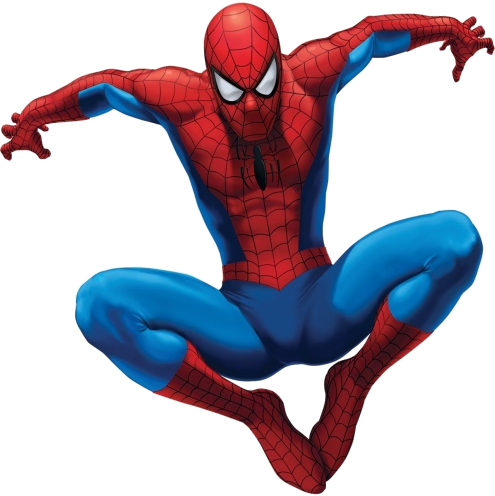
\includegraphics[height=2.9cm]{images/les2-hero-1}};
    \node[anchor=north] (hero2) at (0.8,2.05)
    {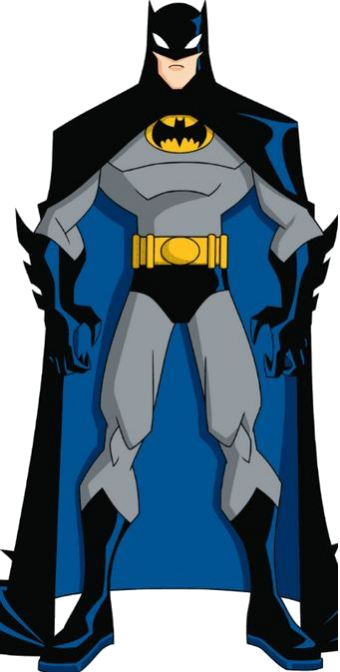
\includegraphics[height=4cm]{images/les2-hero-2}};
    \node[anchor=north] (hero3) at (1.3,1.575)
    {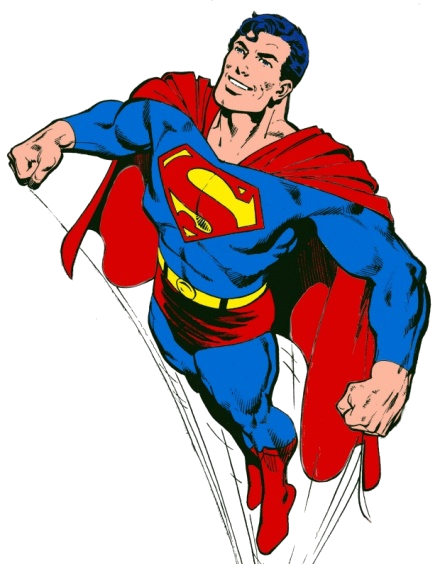
\includegraphics[height=3.1cm]{images/les2-hero-3}};
    \node[anchor=north] (hero4) at (1.8,2.1)
    {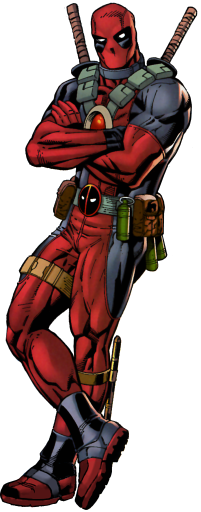
\includegraphics[height=4.1cm]{images/les2-hero-4}};
    \node[anchor=north] (hero5) at (2.3,1.95)
    {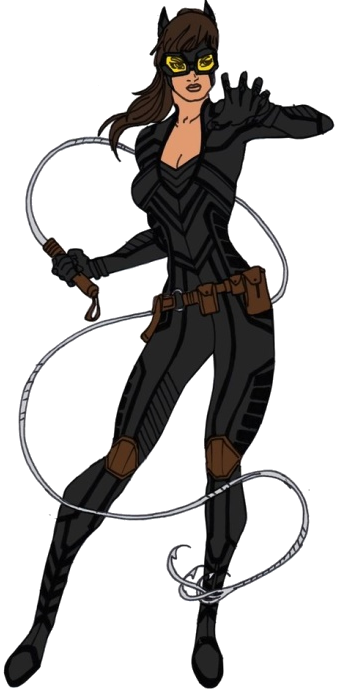
\includegraphics[height=3.8cm]{images/les2-hero-5}};

    \node (size1) at (0.3, 1.5) {\scriptsize 141 cm};
    \node (size2) at (0.8, 2.1) {\scriptsize 198 cm};
    \node (size3) at (1.3, 1.51) {\scriptsize 143 cm};
    \node (size4) at (1.8, 2.15) {\scriptsize 201 cm};
    \node (size5) at (2.3, 1.95) {\scriptsize 184 cm};
  \end{tikzpicture}
  \caption{De superhelden die we onderzoeken}
  \label{fig:superheldenSteekproef}
\end{figure}

\begin{figure}
  \centering
  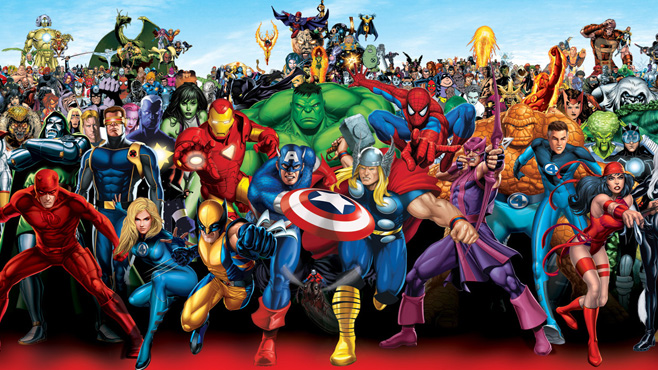
\includegraphics[width=0.85\textwidth]{images/les5-heroes.jpg}
  \caption{Onze superhelden die we onderzoeken vormen een steekproef uit de populatie van alle superhelden.}
  \label{fig:populatieHelden}
\end{figure}

\section{Populatie en Steekproeven}
\begin{definition}[Populatie]
  De verzameling van \textbf{alle} objecten of personen waar men in ge\"interesseerd is en onderzoek naar wil doen noemt men de \index{populatie} populatie. Een ander woord is ook wel onderzoeksgroep of doelgroep.
\end{definition}

\begin{definition}[Steekproef]
  Wanneer met een subgroep uit een populatie gaat onderzoeken, dan noemen we die groep een \index{steekproef} steekproef.
\end{definition}

\begin{definition}[Steekproefkader]
  Een \index{steekproefkader} steekproefkader is een lijst van alle leden van een te onderzoeken populatie.
\end{definition}

Er zijn een aantal redenen waarom een steekproef genomen wordt:
\begin{itemize}
  \item Populatie is te groot om een volledig onderzoek te doen.
  \item Kostbare metingen waardoor het onderzoek te duur wordt.
  \item Wanneer snelheid belangrijk is, is het vaak sneller een subgroep te onderzoeken;
  \item Gemakkelijker \dots
\end{itemize}

Om een steekproef op te zetten volg je volgende stappen:
\begin{enumerate}
  \item \textbf{Definitie populatie}: Wie is er deel van de populatie? Dit hangt nauw samen met de probleemstelling van het onderzoek. Dit is een zeer belangrijke stap waar je niet licht over mag gaan. Elementen die van belang zijn, zijn bijvoorbeeld sociale, demografische of fysieke kenmerken zoals geslacht, leeftijd, woonplaats \dots
  \item \textbf{Bepalen van steekproefkader}: Een populatie heeft verschillende segmenten zoals bijvoorbeeld rijke superhelden, arme superhelden, bekende en onbekende superhelden, superhelden met en zonder oudercomplex \dots In de praktijk is het meestal onmogelijk om de populatie als geheel te onderzoeken. Daarom beperken we ons vaak tot enkele redelijk homogene subpopulaties of segmenten. De populatiesegmenten die daadwerkelijk onderzocht worden noemen we de operationele populatie.
  \item \textbf{Budget en Tijd}: het aantal te onderzoeken objecten of personen zal ook afhankelijk zijn van budget en tijd.
\end{enumerate}

\section{Kiezen van steekproefmethode}
  Soms is de populatie die men wenst te bestuderen erg verschillend op een aantal belangrijke kenmerken. Daartoe wordt de populatie als geheel in een aantal elkaar niet-overlappende en homogene strata of klassen ingedeeld.

\begin{definition}[Gestratificeerde steekproef]
Een \textbf{gestratificeerde} \index{gestratificeerd} steekproef is proportioneel als het aandeel van de subpopulatie in de steekproef gelijk is aan het aandeel van de subpopulatie in de populatie als geheel.
\end{definition}

\begin{example}
  Indien we uit een populatie van de superhelden kijken naar de leeftijd van  mannen en vrouwen, zien we in tabel \ref{tab:heldenPopulatie1} de absolute waarden. We kunnen niet alle superhelden ondervragen, maar indien we een steekproef nemen waarbij de mannen en leeftijdscategorie\"en relatief equivalent zijn met de populatie, hebben we een gestratificeerde steekproef genomen (zie tabel \ref{tab:heldenPopulatie2}).
\end{example}

  \begin{table}
  \centering
    \begin{tabular}{l|cccc|c}
      & \multicolumn{4}{c|}{\textbf{Leeftijd}} & \\
      Geslacht & $\le 18$ & $]18,25]$ & $]25, 40]$ & $> 40$ & Totaal\\
      \hline
      Vrouw & 500 & 1500 & 1000 & 250 & 3250 \\
      Man   & 400 & 1200 & 800 & 160 & 2560\\
      \hline
      Totaal & 900 & 2700 & 1800 & 410 & 5810
    \end{tabular}
    \caption{Frequenties van de superhelden in de populatie volgens geslacht en leeftijdscategorie}
    \label{tab:heldenPopulatie1}
\end{table}

\begin{table}
  \centering
    \begin{tabular}{l|cccc|c}
      & \multicolumn{4}{c|}{\textbf{Leeftijd}} & \\
      Geslacht & $\le 18$ & $]18,25]$ & $]25, 40]$ & $> 40$ & Totaal\\
      \hline
      Vrouw & 50 & 150 & 100 & 25 & 325 \\
      Man   & 40 & 120 & 80 & 16 & 256\\
      \hline
      Totaal & 90 & 270 & 180 & 41 & 581
    \end{tabular}
      \caption{Steekproef van superhelden gestratificeerd volgens geslacht en leeftijdscategorie.}
    \label{tab:heldenPopulatie2}
  \end{table}

Nadat gestratificieerd is, moet bepaald worden op welke wijze binnen ieder stratum het aantal benodigde objecten of respondenten gekozen moet worden. Bij de toevals- of \textbf{aselecte} \index{aselect} steekproeven heeft elk element van de populatie een even mogelijke kans om in de steekproef te worden opgenomen. Dit heeft als gevolg dat je op basis van de data van een aselecte steekproef conclusies kan trekken ten aanzien van de kenmerken van een populatie, en dit in tegenstelling met een \textbf{niet-aselecte} steekproef. In een niet-aselecte steekproef kent men de kans niet dat elk lid van de populatie heeft om in de steekproef terecht te komen, met als gevolg dat je gegevens enkel gelden voor je onderzochte groep.

\subsection{Fouten bij steekproeven}
\subsubsection{Toevallige steekproeffouten}
Wanneer er puur door het toeval een verschil is in een waarde voor de populatie en de steekproef.

\subsubsection{Systematische steekproeffouten}
Een procedure in de steekproef die een fout oplevert die een systematische oorzaak heeft en dus niet te wijten is aan toevallige effecten. Bijvoorbeeld door systematisch een bevoordeeld deel van de populatie te ondervragen. Als we onze superhelden zouden ondervragen via het internet, sluiten we alle superhelden uit die geen internetverbinding hebben.

\subsubsection{Toevallige niet-steekproeffouten}
Hieronder vallen bijvoorbeeld verkeerd aangekruiste antwoorden of verschil in interpretatie van de vragen.

\subsubsection{Systematische niet-steekproeffouten}
Wanneer bijvoorbeeld respondenten met een sterke band met het onderzoek eerder geneigd zijn om een vragenlijst in te vullen, ga je positievere antwoorden krijgen - terwijl ze niet representatief zijn voor de gehele populatie.

\subsection{Aanpassing formules standaarddeviatie}
We noemen het gemiddelde van de steekproef het steekproefgemiddelde en gebruiken hiervoor het symbool $\overline{x}$ (dit hebben we stilzwijgend al een aantal keer gedaan in de vorige hoofdstukken).

Als we de standaardafwijking van een steekproef willen bepalen dan moeten we niet meer delen door $n$ (aantal metingen) maar door $(n-1)$. Waarom?

Aangezien de som van de afwijkingen $x_{i} - \overline{x}$ steeds 0 oplevert (zie hieronder in vergelijking \ref{eq:sumGemid}), kan de laatste afwijking gevonden worden uit de eerste $n-1$ afwijkingen. We berekenen dus niet het gemiddelde van $n$ getallen zonder verwantschap. Slecht $n-1$ van de gekwadrateerde afwijkingen kunnen vrij bewegen, daarom berekenen we het gemiddelde door het totaal te delen door $n-1$. Het getal $n-1$ noemt men het aantal vrijheidsgraden van de variantie of van de standaardafwijking.

\begin{equation}
 \sum_{i}^{n}(x_{i} - \overline{x}) = \sum_{i}^{n}x_{i} - \sum_{i}^{n}\overline{x} = \sum_{i}^{n}x_{i} - n (\frac{1}{n}\sum_{i}^{n} x_{i})
\label{eq:sumGemid}
\end{equation}

\section{Kansverdeling van een steekproef}
\subsection{Stochastisch experiment}
Een random (of stochastisch) experiment heeft volgende elementen nodig:

\begin{definition}[Universum of Uitkomstenruimte]\
 Het universum of uitkomstenruimte van een experiment
is de verzameling van alle mogelijke uitkomsten van dit experiment en
wordt genoteerd met $\Omega$.
\end{definition}
~\\
\textbf{Opmerkingen}
\begin{itemize}
\item De uitkomstenruimte moet \emph{volledig}\/ zijn: elke mogelijke
uitkomst van een experiment moet tot $\Omega$ behoren.
\item Bovendien moet elke
uitkomst van een experiment overeenkomen met \emph{juist \'e\'en}\/ element van
$\Omega$.
\item Samengevat: na het uitvoeren van een experiment is het  mogelijk  om eenduidig
aan te geven welk element van $\Omega$ zich heeft voorgedaan.
\end{itemize}

\begin{definition}[Gebeurtenis]
 Een gebeurtenis is een deelverzameling van de uitkomstenruimte. Een enkelvoudige of elementaire gebeurtenis is een singleton;   een samengestelde gebeurtenis heeft cardinaliteit groter dan 1.
\end{definition}
Gebeurtenissen die geen gemeenschappelijke uitkomsten hebben noemt men
{disjunct. \\
Disjuncte gebeurtenissen kunnen dus nooit samen voorkomen.\\
Wanneer de gebeurtenissen $A$ en $B$ disjunct zijn dan geldt
$A \cap B = \emptyset$.
Startend met
 de gebeurtenissen $A$ en $B$ kan men de volgende gebeurtenissen vormen:
 \begin{itemize}
  \item $A$ \textbf{of} $B$, of wiskundig genoteerd $A \cup B$;
  \item $A$ \textbf{en} $B$, of wiskundig genoteerd $A \cap B$;
  \item \textbf{niet} $A$, of wiskundig genoteerd $\overline{A}$.
\end{itemize}
\textbf{Opmerkingen}
\begin{itemize}
\item Door inductie leidt men gemakkelijk  af dat
de unie van $n$  gebeurtenissen $A_1$ t.e.m.~$A_n$ eveneens
een gebeurtenis is.
\item Idem voor de doorsnede van
gebeurtenissen.
\item Voor sommige toepassingen is het nodig om ook (aftelbaar) oneindige
unies en doorsnedes te beschouwen.
\end{itemize}

\begin{definition}[Kansruimte]
Het toekennen van kansen aan gebeurtenissen dient aan de volgende drie regels te voldoen.
\begin{enumerate}
\item Kansen zijn steeds positief:
 $P(A) \geq 0$ voor elke $A$.
  \item
  De uitkomstenruimte heeft kans 1:
  $P(\Omega) = 1.$
 \item Wanneer $A$ en $B$ \emph{disjuncte}\/ gebeurtenissen zijn dan is
 \[P(A\cup B) = P(A) + P(B). \]
 Dit noemt men de somregel.
\end{enumerate}
Wanneer de functie $P$ aan de bovenstaande eigenschappen (axioma's) voldoet
dan noemt men het drietal $(\Omega, \mathcal{P}(\Omega), P)$ een
kansruimte (met $\mathcal{P}(\Omega)$ de \emph{machtsverzameling} van $\Omega$, d.w.z.~de verzameling van alle deelverzamelingen van $\Omega$).
\end{definition}

\begin{example}
Beschouw een uitkomstenruimte $\Omega =  \left\{ 1,2,3,4,5,6 \right\} $ en
een kansfunctie $P(\omega)=\frac{1}{|\Omega|}$, dan zou dit een dobbelsteen
kunnen voorstellen met uitkomsten 1 tot en met 6 met een kans
$P(\omega) = \frac{1}{6}$ om een van de nummers te werpen.
\end{example}

In dit onderdeel van de  cursus gaan we ons bezig houden met \textbf{inductieve statistiek}: op basis van een getrokken steekproef uitspraken doen over de populatie.

\subsection{Kansverdeling}
\subsubsection{Discrete kansverdeling}
Als we het voorbeeld nemen van het gooien van een dobbelsteen, dan kunnen we de kans dat we een van de getallen $\Omega = \{1,2,3,4,5,6\}$ in een tabel zetten of kunnen er een histogram van maken.  Er zijn een aantal belangrijke opmerkingen hierbij:
\begin{enumerate}
  \item De kansen zijn allemaal groter of gelijk aan nul.
  \item De kans op een getal is gelijk aan de bijbehorende oppervlakte van de staaf.
  \item De totale oppervlakte van alle staven is 1.
\end{enumerate}

Een ander voorbeeld is het gooien van twee dobbelstenen met de mogelijke uitkomst. Je hebt volgens de productregel $6 \times 6 = 36$ mogelijke uitkomsten. Om bijvoorbeeld drie te gooien heb je twee mogelijkheden (kans $P(X=3) = \frac{2}{36}$). Zie voor de andere getallen tot en met 7 de tabel ($ P[X=n] = \frac{n-1}{36}$).

Als we dit nu in een histogram steken bekomen we een mooie trap naar boven tot 7 en dan weer naar beneden. Nu kan je makkelijk zien dat:
\begin{itemize}
  \item Voor de kans om 10 of meer te gooien moet je bijvoorbeeld die blauwe oppervlakte hebben.
  \item Voor de kans op een aantal meer dan 2 maar minder dan 7 moet je de rode oppervlakte hebben.
  \item Voor de kans op een aantal meer dan 7 maar minder dan 10 moet je de groene oppervlakte hebben.
  \item Dan is het ook logisch dat de totale oppervlakte 1 is: de kans dat 1 van al die mogelijkheden voorkomt is natuurlijk 100\%.
\end{itemize}

\subsubsection{Continue kansverdeling}

Continue kansverdelingen zijn verdelingen waarbij hetgeen we meten niet alleen een beperkt aantal waarden kan aannemen (nominaal en ordinaal meetniveau), maar ook alle er tussenliggende waarden (ratio- en intervalniveau). Neem bijvoorbeeld het gewicht van onze superhelden. Dat is continu, immers dat kan niet alleen $60$ of $70$ kilo zijn, maar ook (bij benadering)  $66,8735485653$ kilo. In principe zijn alle tussenliggende waarden mogelijk (al is dat in praktijk vaak niet te meten). Dat heeft een belangrijk gevolg voor de kansverdeling. Die bestaat nu (in theorie) niet meer uit losse staafjes, maar is een vloeiende kromme geworden. Dat betekent dat de kans op bijvoorbeeld precies $70$ kilogram een kans nul heeft. Bij precies $70$ kg hoort een verticaal lijntje, en een lijntje heeft oppervlakte nul. Nu is die kans natuurlijk ook nul. Als we zeggen $70$ kg, dan bedoelen we meestal tussen $69,5$ en $70,5$, of preciezer het interval $[69,5; 70,5[$. Als we zeggen $70,00000$ kg, dan bedoelen we iets als binnen $[70,000005; 69,999995[$ kg.

De twee regels voor kansverdelingen hierboven blijven gewoon geldig. Als zo'n kromme een goede kansverdeling is, dan moet de totale oppervlakte ervan 1 zijn, en dan kun je de kans op een gewicht dat bijvoorbeeld tussen de 60 en 70 kg ligt uitrekenen door de oppervlakte hiernaast te bepalen (merk op dat het uiteindelijk niet belangrijk is of die $60$ en $70$ zelf ook nog tot het interval behoren, die hebben toch kans nul!).

\section{De normale verdeling}

\begin{figure}[t]
\centering
\begin{tikzpicture}
\begin{axis}[
  domain=0:10, samples=100,
  axis lines*=left, xlabel=$x$, ylabel=$y$,
  every axis y label/.style={at=(current axis.above origin),anchor=south},
  every axis x label/.style={at=(current axis.right of origin),anchor=west},
  height=5cm, width=12cm,
  xtick={5,3.5,6.5}, ytick=\empty,
  enlargelimits=false, clip=false, axis on top,
  grid = major
  ]
  \addplot [fill=cyan!20, draw=none, domain=0:9] {gauss(5,1.5)} \closedcycle;
  \draw [yshift=-0.6cm, latex-latex](axis cs:3.5,0) -- node [fill=white] {$\sigma$} (axis cs:6.5,0);
\end{axis}
\end{tikzpicture}
\caption{De kansverdeling van de reactiesnelheid van superman. Deze grafiek noemen we de normaalverdeling met gemiddelde $\mu = 5$ ms en standaarddeviatie $\sigma = 1,5 ms.$}
\label{fig:verdelingReactievermogen}
\end{figure}


In figuur \ref{fig:verdelingReactievermogen} tonen we de kansverdeling van de reactiesnelheid X van superman. Deze grafiek noemen we de normaalverdeling met gemiddelde 5 ms en standaarddeviatie 1,5 ms. Symbolisch:
\[ X  \sim Nor(\mu = 5; \sigma = 1,5) \]

De functie die hiermee gepaard gaat is de volgende:

\begin{equation}
  f(x) = \frac{1}{\sigma \sqrt{2\pi}} e^{-\frac{1}{2} \frac{(x - \mu)^{2}}{\sigma^{2}}}
  \label{eq:normalFunction}
\end{equation}

De normale verdeling kent volgende eigenschappen:
\begin{itemize}
  \item Normale verdeling is klokvormig
  \item De normale verdeling is symmetrisch
  \item Vanwege symmetrie is gemiddelde, mediaan en modus aan elkaar gelijk
  \item De totale oppervlakte onder de klokvormige figuur is 1
  \item In gebied $\sigma$ onder $\mu$ en $\sigma$ boven $\mu$ (het zogenoemde sigma gebied) ligt ongeveer 68\% van de waarnemingen.
  \item In het gebied $2\sigma$ boven en onder $\mu$ ligt ongeveer 95\% van alle waarnemingen.
  \item Voor de verschillende gebieden zie figuur \ref{fig:standaardNormaleVerdeling}
\end{itemize}

\subsection{De standaardnormale verdeling}

Indien de toevalsveranderlijke $X \sim N(\mu,\sigma)$ verdeeld is dan is de toevalsvariabele $Z = \frac{X - \mu}{\sigma}$ normaal verdeeld: $Z \sim N(0,1)$. Dit noemen we de standaardnormale verdeling.

  % Bron: http://johncanning.net/wp/?p=1202
  \begin{center}
  \begin{figure}
  \centering
    \begin{tikzpicture}
      \begin{axis}[
          no markers, domain=0:10, samples=100,
          axis lines*=left,height=6cm, width=10cm,
          xtick={-3, -2, -1, 0, 1, 2, 3}, ytick=\empty,
          enlargelimits=false, clip=false, axis on top,
          grid = major
        ]
        \addplot [smooth,fill=cyan!20, draw=none, domain=-3:3] {gauss(0,1)} \closedcycle;
        \addplot [smooth,fill=orange!20, draw=none, domain=-3:-2] {gauss(0,1)} \closedcycle;
        \addplot [smooth,fill=orange!20, draw=none, domain=2:3] {gauss(0,1)} \closedcycle;
        \addplot [smooth,fill=blue!20, draw=none, domain=-2:-1] {gauss(0,1)} \closedcycle;
        \addplot [smooth,fill=blue!20, draw=none, domain=1:2] {gauss(0,1)} \closedcycle;
        \addplot[<->] coordinates {(-1,0.4) (1,0.4)};
        \addplot[<->] coordinates {(-2,0.3) (2,0.3)};
        \addplot[<->] coordinates {(-3,0.2) (3,0.2)};
        \node[coordinate, pin={68.2\%}] at (axis cs: 0, 0.35){};
        \node[coordinate, pin={95\%}] at (axis cs: 0, 0.25){};
        \node[coordinate, pin={99.7\%}] at (axis cs: 0, 0.15){};
        \node[coordinate, pin={34.1\%}] at (axis cs: -0.5, 0){};
        \node[coordinate, pin={34.1\%}] at (axis cs: 0.5, 0){};
        \node[coordinate, pin={13.6\%}] at (axis cs: 1.5, 0){};
        \node[coordinate, pin={13.6\%}] at (axis cs: -1.5, 0){};
        \node[coordinate, pin={2.1\%}] at (axis cs: 2.5, 0){};
        \node[coordinate, pin={2.1\%}] at (axis cs: -2.5, 0){};
      \end{axis}
    \end{tikzpicture}
    \caption{De standaardnormale verdeling met opdeling in zones}
    \label{fig:standaardNormaleVerdeling}
    \end{figure}
  \end{center}

In het algemeen kan dus bij een waarneming $x$ de zogenaamde $z$-score bepalen als volgt:

\begin{equation}
  z = \frac{x-\mu}{\sigma}
  \label{eq:zscore}
\end{equation}

Deze score geeft dus aan hoe extreem een waarneming is of anders gezegd, hoeveel standaarddeviaties is de waarneming $x$ van het gemiddelde $\mu$ verwijderd. Voor een willekeurige $x$-waarde kunnen we met formule \ref{eq:zscore} de bijhorende $z$-score bepalen. Voor deze $z$-scores heeft men tabellen opgesteld met de kansen dat een waarde kleiner dan $z$ getrokken wordt uit Z, de zgn.~linkerstaartkans\footnote{Er bestaan ook tabellen met de rechterstaartkans}: $P(Z<z)$.

R heeft eveneens functies voor het rekenen met kansen van normaal verdeelde variabelen. Deze worden samengevat in Tabel~\ref{rab:norm-prob-r}.

\begin{table}
  \centering
  \begin{tabular}{ll}
  	\textbf{Functie}      & \textbf{Betekenis}                                             \\ \hline
  	\verb|pnorm(x, m, s)| & Linkerstaartkans, $P(X<\mathtt{x})$                            \\
  	\verb|dnorm(x, m, s)| & Hoogte van de Gausscurve op punt \texttt{x}                    \\
  	\verb|qnorm(p, m, s)| & Onder welke grens zal \texttt{p}\% van de waarnemingen liggen? \\
  	\verb|rnorm(n, m, s)| & Genereer \texttt{n} normaal verdeelde random getallen
  \end{tabular}
  
  \caption{Kansberekeningsfuncties in R voor een normale verdeling met gemiddelde \texttt{m} en standaardafwijking \texttt{s}. Indien argumenten \texttt{m} en \texttt{s} weglaten worden, wordt de standaardnormaalverdeling verondersteld.}
  \label{rab:norm-prob-r}
\end{table}

We komen dan tot de volgende methode voor het berekenen van kansen met de normale verdeling:
\begin{enumerate}
  \item Bepaal de kansvariabele met de bijbehorende normale verdeling
  \item Bereken de $z$-score bij de bijhorende $x$-waarde.
  \item Schets de plaats van de gevraagde kans
  \item Herleid de gevraagde kans met behulp van de schets tot een linkerstaartkans en gebruik de $z$-tabel van de standaardnormale verdeling om deze te bepalen. Gebruik indien nodig de symmetrieregel en de regel van 100\% kans.
\end{enumerate}

\begin{example}
Hoe groot is de kans dat superman in minder dan 4 ms reageert?
\[ P(X < 4) = P(Z < -0,67) = 0,2514 \]
\end{example}
\begin{example}
Hoe groot is de kans dat hij in minder dan 7 ms reageert?
\[ P(X < 7) = P(Z < 1,33) = 0,9082 \]
\end{example}
\begin{example}
Hoe groot is de kans dat superman in minder dan 3 ms reageert?
\[ P(X<3) = P(Z < -1,33) = 0,0918 \]
\end{example}
\begin{example}
Hoe groot is de kans dat hij reageert tussen de 2 en 6,5 ms
\[ P( 2 < X < 6,5) = P(X<6,5) - P(X<2) = P(Z<1) - P(Z<-2) = 0,8186 \]
\end{example}

\subsection{Testen op normaliteit}

Er zijn verschillende methoden die kunnen gebruikt worden om na te gaan of een steekproef uit een normale verdeling komt.
\begin{enumerate}
  \item Construeer een histogram voor de gegevens en bekijk de vorm van de grafiek. Als de gegevens bij benadering een normale verdeling hebben, zal de vorm van het histogram een klokcurve vormen.
  \item Bereken de intervallen $\overline{x} \pm s$, $\overline{x} \pm 2s$, $\overline{x} \pm 3s$ en bepaal het percentage meetwaarden dat binnen elk van deze intervallen valt. Als de gegevens ongeveer normaal verdeeld zijn, zullen de percentages ongeveer gelijk zijn aan respectievelijk 68\%, 95\% en 99,7\%.
  \item Construeer een QQ-plot (normaliteitsplot, zie Definitie~\ref{def:qq-plot}) voor de gegevens. Als de gegevens ongeveer normaal verdeeld zijn, zullen de punten ongeveer op een rechte lijn liggen.
  \item Bereken de \emph{kurtosis} (``welving'' of ``platheid''): duidt aan hoe scherp de ``piek'' van de verdeling is.
    \begin{itemize}
      \item Een normale verdeling heeft een kurtosis = 0
      \item Een vlakke distributie heeft een negatieve kurtosis
      \item Een eerder piekvormige distributie heeft een positieve kurtosis
      \item Let op: bij de originele definitie van kurtosis (zoek die eens op!) heeft de normale verdeling een kurtosis van 3. Wij gebruiken hier een alternatieve definitie, meestal de ``excess kurtosis'' genoemd, waar men 3 aftrekt van de originele waarde, zodat je op 0 uitkomt.
    \end{itemize}
  \item Berken de \emph{Skewness} (scheefheid): duidt aan hoe symmetrisch de data is.
    \begin{itemize}
      \item Een symmetrische distributie heeft een skewness = 0
      \item Bijgevolg: een normale verdeling heeft een skewness = 0.
      \item Een distributie met een lange linkerstaart heeft een negatieve skewness
      \item Een distributie met een lange rechterstaart heeft een positieve skewness
      \item Vuistregel: absolute waarde van skewness $>1$, geen symmetrische distributie.
    \end{itemize}
\end{enumerate}

\begin{definition}[QQ-plot of normaliteitsplot]
  \label{def:qq-plot}
  Een normaliteitsplot of QQ-plot\footnote{Q staat hier voor \emph{quantile}, kwantiel} voor een gegevens\-verzameling is een spreidingsdiagram met de gesorteerde gegevenswaarden op de ene as en de bijbehorende verwachte $z$-waarden van een standaardnormale verdeling op de andere as. Zie figuur~\ref{fig:qqplot} voor enkele voorbeelden. De R-code voor het genereren van deze afbeeldingen is hieronder gegeven.
\end{definition}

\begin{figure}
  \begin{center}
    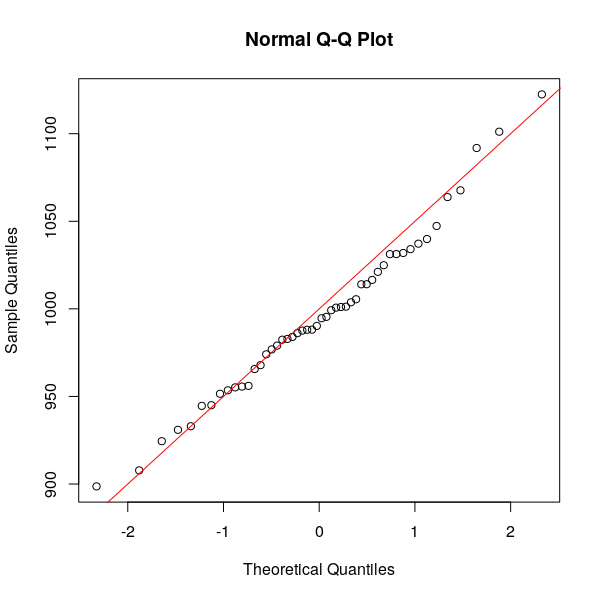
\includegraphics[width=.45\textwidth]{sampling-qqplot-good}
    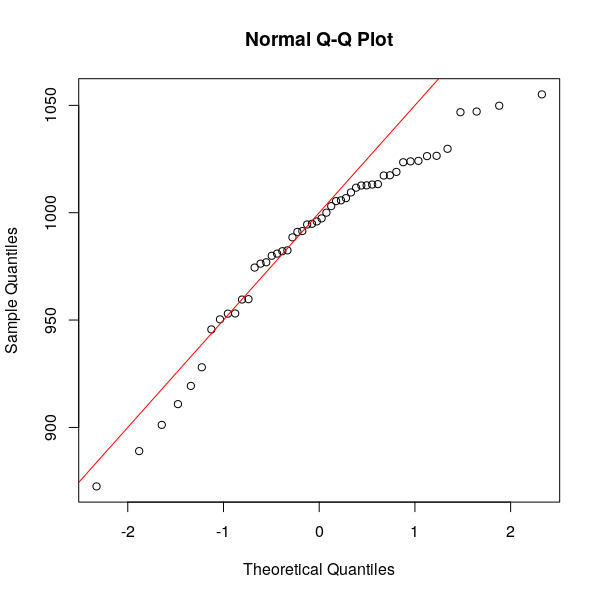
\includegraphics[width=.45\textwidth]{sampling-qqplot-bad}
  \end{center}
  \caption{De QQ-plot links is gebaseerd op een steekproef van 50 observaties uit een normale distributie met gemiddelde 1000 en standaardafwijking 50. De rechterplot is gebaseerd op een Student-$t$ distributie met 15 vrijheidsgraden. Het aantal observaties, gemiddelde en standaardafwijking zijn hetzelfde als links.
    De lijnen in het rood duiden aan waar zich in theorie de observaties zouden moeten bevinden. Links is dat min of meer zo, maar rechts wijken de observaties af, vooral in de extremen.}
  \label{fig:qqplot}
\end{figure}

\lstinputlisting{data/qqplot.R}

\subsection[Chi-kwadraatverdeling]{$\chi^{2}$ verdeling}
Laat $X_{1}, X_{2}, \dots X_{v}$ onafhankelijk standaardnormale variabelen zijn ($\sim N(0,1)$). De $\chi^{2}$ (chi-kwadraat) variabele wordt als volgt gedefinieerd:
\[ \chi^{2}_{v} = X_{1}^{2} + X_{2}^{2} + \dots + X_{v}^{2} \]

Het getal $v$ noemt men het aantal vrijheidsgraden van de variabele. $\chi^{2}$ is een continue toevalsveranderlijke, die positief is omdat ze de som is van kwadraten. Haar dichtheidsfunctie is de volgende:

\[ f_{n}(x) = \frac{1}{2^{\frac{n}{2}}\Gamma(\frac{n}{2})} x^{\frac{n}{2} -1} e^{\frac{x}{2}} \]

De verwachtingswaarde (= gemiddelde) is $v$ en zijn variantie is $2v$. Zijn modus voor $v \geq 2$ is $v-2$.

De $\chi^{2}$ variabele komt niet in de natuur voor. Geen verschijnsel kan erdoor gemodelleerd worden. maar deze variabele zal zeer belangrijk zijn in het vervolg van de cursus.

\section{Centrale limietstelling}
\label{sec:centrale-limietstelling}

\begin{definition}[Lineaire combinatie van onafhankelijke, gelijk verdeelde stochasten]
Formeel: Een lineaire combinatie van onafhankelijke, gelijk verdeelde stochasten is steeds normaal verdeeld.

\[X_{i} \sim Nor(\mu_{i}, \sigma_{i}) \Rightarrow Y = \sum_{i} \alpha_{i} X_{i} \textnormal{ ook normaal verdeeld} \]

Bijgevolg zal ook het steekproefgemiddelde van een steekproef uit een populatie met een willekeurige verdeling, nagenoeg normaal verdeeld zijn voor een voldoende grote $n$.
\end{definition}

Wanneer men dus een aselecte steekproef neemt van onafhankelijke variabelen met een normale verdeling, dan zegt de centrale limietstelling dat het gemiddelde van deze steekproef bij benadering normaal verdeeld zal zijn. Dus als men steeds opnieuw een steekproef neemt met dezelfde grootte, en telkens het gemiddelde optekent, bekomt men bij benadering de grafiek van een normale verdeling. Hoe groter de steekproef, hoe beter de benadering. Het steekproefgemiddelde is dus normaal verdeeld, onafhankelijk van de onderliggende verdeling van de grootheid waarvan men een steekproef neemt. Algemeen kunnen we volgende stelling poneren:

\begin{definition}[Centrale limietstelling]
Beschouw een aselecte steekproef van $n$ waarnemingen die uit een populatie met verwachtingswaarde $\mu$ en standaardafwijking $\sigma$ wordt genomen. Als $n$ groot genoeg is zal de kansverdeling van het steekproefgemiddelde $\overline{x}$ een normale verdeling benaderen met verwachting $\mu_{\overline{x}} = \mu$ en standaardafwijking $\sigma_{\overline{x}} = \frac{\sigma}{\sqrt{n}}$. Hoe groter de steekproef is, des te beter zal de kansverdeling van $\overline{x}$ de verwachtingswaarde van de populatie benaderen.

\end{definition}

Bij het afnemen van een steekproef is zelden de onderliggende verdeling gekend, en toch kan men uitspraken doen over de gemiddelde waarde. Dit is volledig te danken aan de centrale limietstelling, die dit gemiddelde een regel oplegt los van de onderliggende kansverdeling. De centrale limietstelling houdt het steekproefgemiddelde in bedwang, sluit het op in de Gaussische kooi waaruit het nooit kan ontsnappen. Dit, en alleen dit, laat wetenschappers toe het nauwkeurig te bestuderen, te observeren en stelt hen in staat te concluderen.

Want, mocht de verdeling van het steekproefgemiddelde afhankelijk zijn van de onderliggende verdeling, een resultaat dat men tot op zekere hoogte zelfs zou verwachten, zou het onmogelijk zijn om concrete uitspraken te doen over vele wetenschappelijke resultaten. In de theoretische statistiek duiken vrijwel constant limieten van steekproefgemiddeldes op, en deze kunnen dankzij de centrale limietstelling zonder verpinken vervangen worden door een normale verdeling. Zou dit niet mogelijk zijn, dan zou de ganse theorie rond het schatten van parameters in elkaar storten wat dan weer rampzalig zou zijn voor de praktijk. Onderzoeken vergelijken zou herleid worden tot een quasi onmogelijke opgave, en de statistiek in het algemeen zou veel lastiger en ingewikkelder worden.

\subsection{Toepassing van de centrale limietstelling}
Bij het trekken van een aselecte steekproef van omvang $n$ uit een populatie met (onbekend) gemiddelde $\mu$ en standaarddeviatie $\sigma$ is de kansverdeling van het steekproefgemiddelde een kansvariabele $M \sim N (\overline{x}, \frac{\sigma}{\sqrt{n}})$, op voorwaarde dat de steekproefomvang voldoende groot is.

\begin{example}
  We bekijken nu de reactiesnelheid van al onze superhelden en uit onze steekproef met $n = 100$ en $\overline{x} = 90, \sigma = 90$ (miliseconden). Dan kunnen we ons de vraag stellen: wat is de kans dat de gemiddelde reactiesnelheid van een superheld minder is dan $104 ms$?


  \begin{enumerate}
    \item De kansvariabele hier is de gemiddelde reactiesnelheid $\overline{x}$ in een steekproef van $n=100$ superhelden. Daarom geldt wegens de centrale limietstelling:
    \[ \overline{x} \sim Nor(\mu = 90, \sigma_{\overline{x}} = \frac{60}{\sqrt{100}} = 6) \]
    \item We kunnen hierbij de passende $z$-score bepalen:
    \[ z = \frac{104-90}{\frac{60}{\sqrt{100}}} = \frac{104-90}{6} = 2,33 \]
    Dus geldt : $P(\overline{x} < 104) = P(Z < 2,33) = 1 - 0,0099 \approx 0,99$
  \end{enumerate}
\end{example}

\subsection{Schatten van een parameter}
Indien we nu een steekproef onderzoeken, willen uit de berekening op de steekproef een aantal conclusies kunnen trekken met betrekking tot de populatie. We willen bijvoorbeeld de gemiddelde kracht kennen van een superheld of de fractie superhelden die rijk zijn. Als we een schatting geven voor dergelijke onbekende parameter, noemen we dat ook een puntschatter. We gebruiken bijvoorbeeld $\overline{x}$ als schatter om $\mu$ te schatten.

\begin{definition}[puntschatter]
  Een puntschatter voor een populatieparameter is een regel of een formule die ons zegt hoe we uit de steekproef een getal moeten berekenen om de populatieparameter te schatten. Een puntschatter is dus een steekproefgrootheid.
\end{definition}

\subsection{Betrouwbaarheidsinterval populatiegemiddelde bij grote steekproef}

In het geval het schatten van een gemiddelde van een populatie uit een steekproef hebben we totaal geen idee over hoe correct onze schatting is. Daarvoor gaan we op zoek naar een interval waarvan we met een bepaalde zekerheid, bv. 95\%, kunnen zeggen dat het de te schatten karakteristiek bevat.

\begin{definition}[Betrouwbaarheidsinterval]
Een betrouwbaarheidsinterval is een regel of een formule die ons zegt hoe we uit de steekproef een interval moeten berekenen dat de waarde van de parameter met een bepaalde hoge waarschijnlijkheid bevat.
\end{definition}

Een eerste goede schatting voor populatiegemiddelde zou het steekproefgemiddelde zijn:

\[ \overline{x} = \frac{1}{n} \sum_{i} x_{i} \]

Natuurlijk is deze schatting niet de werkelijke waarde van de populatie. Daarom wordt vaak rondom $\overline{x}$ een interval geconstrueerd dat de waarden bevat die aannemelijk zijn voor $\mu$. Hiervoor kunnen we gebruik maken van de centrale limietstelling: het gemiddelde in een te trekken steekproef van omvang $n$ is normaal verdeeld met karakteristieken $\mu$ en $\frac{\sigma}{\sqrt{n}}$.  Als we nu het gemiddelde standaardiseren krijgen we:

\[ Z = \frac{\overline{x} - \mu}{\frac{\sigma}{\sqrt{n}}} \]
 Deze uitdrukking hangt van $\mu$ af maar we weten wel dat deze standaardnormaal verdeeld is. We kunnen daarom getallen $-z$ en $z$ vinden, onafhankelijk van $\mu$, waartussen $Z$ met een voorgeschreven kans $1 - \alpha$ ligt. De betrouwbaarheid $1 - \alpha$ geeft aan hoe betrouwbaar we het interval vinden. We nemen hier $1 - \alpha= 0,95$.

\[P(-z < Z < z) = 1 - \alpha = 0,95 \]

Hieruit halen we dat $\alpha = 0,05$. Door het toepassen van de symmetrieregel weten we dus dat we volgende term moeten berekenen:

\[ P( Z < z) = 0,025 \]

Kijken we in de Z-tabel dan vinden we voor de rechterstaartkans $0,025$ de z-score van $1,96$.

Dus vinden we :

\[ P( -1,96 < \frac{\overline{x} - \mu}{\frac{\sigma}{\sqrt{n}}} < 1,96 ) \]
en dus
\[ P ( \overline{x} -1,96 \frac{\sigma}{\sqrt{n}} <\mu < \overline{x} + 1,96 \frac{\sigma}{\sqrt{n}}) \]

Op die manier kunnen we dus grenzen bepalen die een interval aanduidt waar 95\% kans is dat $\mu$ gevonden wordt. Formeel: als je herhaalde steekproeven zou nemen en telkens op basis van het gerealiseerde steekproefgemiddelde $\overline{x}$ een betrouwbaarheidsinterval zou maken, dan zal bij 95\% van de intervallen $\mu$ binnen de intervalgrenzen liggen.

Opgelet, we gaan er hier van uit dat we de standaarddeviatie van de populatie kennen, wat meestal niet zo is. Indien de steekproef groot genoeg is, kunnen we de steekproefstandaarddeviatie nemen als schatter voor de standaarddeviatie voor de populatie.

\[ P ( \overline{x} -1,96 \frac{\sigma_{\overline{x}}}{\sqrt{n}} < \mu < \overline{x} + 1,96 \frac{\sigma_{\overline{x}}}{\sqrt{n}}) \]


\begin{figure}[t]
\centering
\begin{tikzpicture}
\begin{axis}[
  domain=-3:3, samples=100,
  axis lines*=left, xlabel=$z$,
  every axis y label/.style={at=(current axis.above origin),anchor=south},
  every axis x label/.style={at=(current axis.right of origin),anchor=west},
  height=5cm, width=12cm,
  xtick={-1.96,0,1.96}, ytick=\empty,
  enlargelimits=false, clip=false, axis on top,
  grid = major
  ]
  \addplot [fill=cyan!20, draw=none, domain=-3:3] {gauss(0,1)} \closedcycle;
  \draw [yshift=-0.6cm, latex-latex](axis cs:-1.96,0) -- node [fill=white] {$\sigma$} (axis cs:1.96,0);
\end{axis}
\end{tikzpicture}
\caption{Standaardnormale verdeling die 95\% betrouwbaarheidsinterval aanduidt.}
\label{fig:verdelingStandaardnormaal}
\end{figure}

\subsection{Betrouwbaarheidsinterval populatiegemiddelde bij een kleine steekproef}

Bij kleine steekproeven kunnen we niet langer veronderstellen dat de kansverdeling van $\overline{x}$ bij benadering
normaal verdeel is, omdat de centrale limietstelling alleen normaliteit garandeert voor grote steekproeven ($n >30$). De vorm
van de kansverdeling van het steekproefgemiddelde $\overline{x}$ hangt nu af van de vorm van de verdeling van de populatie waaruit de
steekproef genomen wordt. Alhoewel nog steeds geldt dat $\sigma_{\overline{x}} = \frac{\sigma}{\sqrt{n}}$ kan
de standaardafwijking $s$ een slechte benadering zijn voor $\sigma$ als de steekproef klein is.

Als oplossing kunnen we een nieuwe grootheid bepalen. In plaats van

\[ z = \frac{\overline{x} - \mu}{\frac{\sigma}{\sqrt{n}}} \]

construeren we

\[ t = \frac{\overline{x} - \mu}{\frac{s}{\sqrt{n}}} \]

Deze heeft een kansverdeling die beschreven wordt door een Student-t verdeling. Deze lijkt zeer goed op de normale verdeling: klokvormig, symmetrisch en met verwachtingswaarde 0.

De precieze vorm van de kansverdeling $t$ hang af van de steekproefomvang $n$. We zeggen dat de t-verdeling $(n-1)$ vrijheidsgraden heeft (afgekort $df$).
Merk op dat:
\begin{itemize}
  \item $(n-1)$ ook gebruikt werd om $s^{2}$ te berekenen
  \item als $n \rightarrow \infty$ we de standaardnormale verdeling verkrijgen.
\end{itemize}

Indien we nu een betrouwbaarheidsinterval willen bepalen voor een steekproef met een klein aantal waarden moeten we het volgende doen:

\begin{definition}[Betrouwbaarheidsinterval kleine steekproef]
  Om een betrouwbaarheidsinterval voor het gemiddelde te bepalen op basis van een klein steekproef bepalen we:
  \[ \overline{x} \pm t_{\frac{\alpha}{2}}(\frac{s}{\sqrt{n}}) \]
  waarbij $t_{\frac{\alpha}{2}}$ gebaseerd is op $(n-1)$ vrijheidsgraden. We veronderstellen wel dat we een aselecte steekproef genomen hebben uit
  een populatie die bij benadering normaal verdeeld is.
\end{definition}

\begin{table}
  \centering
  \begin{tabular}{ll}
  	\textbf{Functie} & \textbf{Betekenis}                                             \\ \midrule
  	\verb|pt(x, df)| & Linkerstaartkans, $P(X<\mathtt{x})$                            \\
  	\verb|dt(x, df)| & Hoogte van de curve op punt \texttt{x}                         \\
  	\verb|qt(p, df)| & Onder welke grens zal \texttt{p}\% van de waarnemingen liggen? \\
  	\verb|rt(n, df)| & Genereer \texttt{n} random getallen volgens deze verdeling
  \end{tabular}

  \caption{Kansberekeningsfuncties in R voor de Student-$t$ verdeling met \texttt{df} vrijheidsgraden, verwachte waarde 0 en standaardafwijking 1.}
  \label{tab:t-prob-r}
\end{table}

\subsection{Betrouwbaarheidsinterval voor populatiefractie bij een grote steekproef}

Indien je een variabele wil meten als een fractie, bijvoorbeeld \% mensen die ja geantwoord heeft op een bepaalde vraag, dan willen we in feite de kans $p$ op succes in een binomiaal experiment schatten, waarbij $p$ de kans is dat een willekeurig geselecteerde respondent (of element van de populatie) een succes is (succes in termen van binomiaal experiment). We kunnen $p$ dan schatten door bijvoorbeeld:

\[ \overline{p} = \frac{\textnormal{aantal successen}}{n} \]

Om nu de betrouwbaarheid van de schatter $\overline{p}$ te bepalen moeten we de kansverdeling kennen van $\overline{p}$. Dit kunnen we beredeneren door toepassing van de centrale limietstelling op het gemiddelde aantal successen in de steekproef van omvang $n$. Indien succes = 1 en faling = 0, dan hebben we een steekproef van $n$ elementen, ieder met dezelfde verdeling (kans op 1 is $p$ en kans op 0 is $q=1-p$).  Het gemiddelde $\overline{p}$ heeft dan bij benadering een normale verdeling. Of dus:

\begin{itemize}
  \item Verwachting van kansverdeling van $\overline{p}$ is $p$.
  \item De standaardafwijking van kansverdeling $\overline{p} = \sqrt{\frac{pq}{n}}$
  \item Voor grote steekproeven is $\overline{p}$ bij benadering normaal verdeeld.
\end{itemize}

Aangezien $\overline{p}$ een steekproefgemiddelde is van het aantal successen, stelt dit ons in staat een betrouwbaarheidsinterval te berekenen analoog als die voor de intervalschatting van $\mu$ voor grote steekproeven.

\begin{definition}[Betrouwbaarheidsinterval voor $p$ gebaseerd op grote steekproef]
  \[ \overline{p} \pm z_{\frac{\alpha}{2}} \sqrt{\frac{\overline{p}\overline{q}}{n}} \]
  met $\overline{p} = \frac{x}{n}$ en $\overline{q} = 1- \overline{p}$
\end{definition}

\section{Oefeningen}
\label{sec:steekproefonderzoek-oefeningen}

\begin{exercise}
  Een onderzoeker wil zo correct mogelijk de consumptiegewoontes van de inwoners van 18 jaar en ouder in een bepaalde gemeente, met 3 woonkernen, onderzoeken.  Hij onderscheidt 4 leeftijdsgroepen zodat hij uiteindelijk aan 12 deelgroepen komt. Hij vraagt de procentuele samenstelling van de bevolking op in de gemeente en berekent daaruit hoeveel bevragingen hij per deelgroep moet uitvoeren.  Dit noemen we een \emph{quotasteekproef}.
  
  Vragen:
  \begin{enumerate}[label=\alph*.]
    \item Wat zijn de voor- en nadelen?
    \item Welke soort fouten kunnen hier gemaakt worden?
    \item Welke andere parameters zouden kunnen gebruikt worden bij het opsplitsen in deelgroepen?
  \end{enumerate}
\end{exercise}

\begin{exercise}
  Een onderzoeksbureau wil het aankoopgedrag van wasprodukten nagaan. Men beslist een aantal vragen te stellen aan vrouwen tussen de 25 en 55 jaar omdat men ervan uitgaat dat de relevante populatie uit deze categorie consumenten bestaat. 
  
  Vraag:
  
  \begin{enumerate}[label=\alph*.]
    \item Welke fout wordt hier gemaakt? 
    \item Hoe groot is de impact van deze fout?
  \end{enumerate}
\end{exercise}

\begin{exercise}
  	De vakbonden willen een onderzoek doen naar de werkomstandigheden van de werknemers van een IT-bedrijf. Dat bedrijf heeft in totaal 3200 werknemers die verdeeld zijn over 
  12 vestigingen. Omdat het aantal werknemers groot is worden aselect 40 werknemers gekozen per vestiging. De steekproefomvang is dus $n = 480$.	
  \begin{enumerate}[label=\alph*.]
    \item Welk bezwaar kan tegen deze steekproefprocedure worden gebracht?
    \item Wanneer zou dit geen bezwaar zijn?
  \end{enumerate}
\end{exercise}

\begin{exercise}
  We willen een onderzoek voeren naar onze studenten aan de Hogeschool Gent, faculteit Bedrijf en Organisatie. Hiervoor worden de aanwezige studenten in een bepaald opleidingsonderdeel bevraagd.
  
  \begin{enumerate}[label=\alph*.]
    \item Welke kritiek kan je op deze methode geven?
    \item Stel dat de aanwezige docent een kernvak geeft, zeer streng is en tijdens de bevraging rondloopt. Welk bezwaar kan hier gegeven worden?
    \item Stel dat de bevraging niet tijdens een les, maar na een examen gehouden wordt. Welke kritiek kan je op deze methode geven?
  \end{enumerate}
\end{exercise}

\begin{exercise}
  Bereken met behulp van de tabel van de normale verdeling de volgende kansen door de gevraagde kans te herleiden tot een linkerstaartkans. Teken ook elke keer het gevraagde gebied.
  \begin{enumerate}[label=\alph*.]
    \item $P(Z < 1.33)$
    \item $P(Z > 1.33)$
    \item $P(Z < -1.33)$
    \item $P(Z > -1.33)$
    \item $P(Z < 0.45)$
    \item $P(Z > -1.05)$
    \item $P(Z < 0.65)$
    \item $P(-0.45 < Z < 1.20)$
    \item $P(-1.35 < Z < -0.10)$
    \item $P(-2.10 < Z < -0.90)$
  \end{enumerate}
\end{exercise}

\begin{exercise}
  In de  Hogeschool zijn er twee klassen voor het vak onderzoekstechnieken. De studenten werden willekeurig over de klassen verdeeld, zodat we mogen veronderstellen dat de ene klas niet slimmer is dan de andere. In de A-klas geeft mevr. X les, in de B-klas geeft mr. Y les. X is nogal streng en op het einde van het schooljaar behaalt haar klas een gemiddelde van 54 op 100 met een standaardafwijking van 11.

  Y is iets losser en stimuleert de leerlingen al gauw met een puntje meer. Op het einde van het schooljaar behaalt zijn klas een gemiddelde van 62 op 100 en een standaardafwijking van 7.

  Wouter zit in de A-klas en heeft $\frac{63}{100}$ voor wiskunde. Stijn zit in de B-klas en behaalt $\frac{67}{100}$. Wie heeft volgens jou het beste gescoord?
\end{exercise}

\begin{exercise}
  Een gezondheidsonderzoek tussen 1988 en 1994 gaf aan dat de gemiddelde cholesterolwaarde bij vrouwen tussen 20 en 29 jaar 183 mg/dl bedroeg, met een standaardafwijking gelijk aan 36. We nemen nu een aselecte steekproef van 81 vrouwen. Los volgende vragen op:
  
  \begin{enumerate}[label=\alph*.]
    \item Schets de kansdichtheidsfunctie voor de populatie en de kansverdeling van het steekproefgemiddelde $\overline{x}$.
    \item Bepaald de kans dat $\overline{x}$ kleiner is dan 185.
    \item Bepaal de kans dat $\overline{x}$ tussen 175 en 185 ligt.
    \item Bepaal de kans dat $\overline{x}$ groter is dan 190. 
  \end{enumerate}
\end{exercise}

\begin{exercise}
  Een aselecte steekproef van 64 stuks wordt getrokken uit een populatie met onbekende verdeling. De verwachting en de standaardafwijking van de populatie
  zijn wel gekend: $\mu = 20$ en $\sigma=16$. Los volgende vragen op:
  
  \begin{enumerate}[label=\alph*.]
    \item Bepaal de verwachting en standaardafwijking van het steekproefgemiddelde.
    \item Beschrijf de vorm van de verdeling van het steekproefgemiddelde. In hoeverre hangt je antwoord af van de grootte van de steekproef?
    \item Bereken de $z$ score bij $\overline{x_{1}} = 15.5$ en $\overline{x_{2}} = 23$.
    \item Bepaal kans dat $\overline{x} <16$.
    \item Bepaal kans dat $\overline{x} > 23$.
    \item Bepaal kans dat $16< \overline{x}< 22$.
  \end{enumerate}
\end{exercise}

\begin{exercise}
  Verkeersdrempels zijn bedoeld om de snelheid van automobilisten te be\"invloeden. Afhankelijk van de gewenste snelheid in een straat worden de drempels steiler of minder steil gemaakt. Drempel A is zo ontworpen dat 85 \% van de automobilisten de drempel passeert met een snelheid van minder dan 50 km per uur. In de praktijk blijkt dat de passeersnelheid bij een drempel normaal verdeeld is. Bij drempel A werd een gemiddelde passeersnelheid van 43,1 km/h gevonden met standaardafwijking 6,6 km/h.
  
  \begin{enumerate}[label=\alph*.]
    \item Toon aan dat 85\% van de automobilisten niet harder dan 50 km/h rijdt.
    \item Bij hoeveel van de 1200 metingen kan, op grond van eerdere ervaringen, een snelheid van meer dan 55 km/h worden verwacht?
  \end{enumerate}
\end{exercise}

\begin{exercise}
  Gegeven 20 examenresultaten in Tabel~\ref{tab:examen}. Uit resultaten van de laatste jaren blijkt dat $\sigma = 2.45$.
  
  \begin{enumerate}[label=\alph*.]
    \item Wat is $\sigma_{\overline{x}}$ , de standaardafwijking van $\overline{x}$?
    \item Geef het 92\% betrouwbaarheidsinterval voor $\mu$.
    \item Kunnen we er zeker van zijn dat het gemiddeld resultaat minder dan 12.5 bedraagt?
  \end{enumerate}
\end{exercise}

\begin{table}
  \centering
  \begin{tabular}{llllllllll}
    11.5 & 16.5 & 11 & 17.3 & 10.8 & 5.6  & 13.1 & 11.5 & 14.2 & 12.9 \\
    8.7  & 9.2  & 15 & 14.4 & 10   & 10.3 & 18.3 & 12.9 & 14.2 & 8.7 
  \end{tabular}
  \caption{Examenresultaten}
  \label{tab:examen}
\end{table}

\begin{exercise}
  Een schoenhandelaar voert een marktonderzoek uit bij 500 klanten. Daaruit blijkt dat 30\% van hen minstens éénmaal per jaar sportschoenen koopt.  Op basis van secundaire informatie weet hij dat het nationaal gemiddelde op 26\% ligt.  Hij vraagt zich nu af in hoeverre zijn zaak in dat opzicht afwijkt van de nationale norm? (We werken met $\alpha= 5\%$, tweezijdig.)
\end{exercise}

\begin{exercise}
  Een conservenfabrikant krijgt de laatste tijd klachten over de netto inhoud van zijn conserven met wortelen en erwtjes, die volgens de verpakking netto 1 liter zouden moeten bevatten. Daarom laat hij een steekproef nemen waarin de netto inhoud van 40 willekeurig gekozen blikjes wordt gecontroleerd. De resultaten worden samengevat in Tabel~\ref{tab:Steekproefwaarden}.

Vraag A: 
\begin{itemize}
  \item Vul de tabel aan met de cummulatieve absolute frequentie
  \item Vul de tabel aan met de relatieve frequentie
  \item Vul de tabel aan met de cummulatieve relatieve frequentie.
\end{itemize}
Vraag B:

\begin{itemize}
  \item Bereken het gemiddelde
  \item Bereken de standaardafwijking
  \item Hoeveel procent van de blikken bevatten te weinig wortelen en erwtjes.
  \item Teken een histogram van de absolute frequentie.
  \item Zijn de gegevens normaal verdeeld?  Hoe zie je dat?
\end{itemize}

\end{exercise}

  \begin{table}
  \centering
  \begin{tabular}{lr}
    \toprule
    Inhoud & $n_{i}$ \\
    \midrule
    $[970,980[$ & 3 \\
    $[980,990[$ & 5 \\
    $[990,1000[$ & 13 \\
    $[1000,1010[$ & 11 \\ 
    $[1010,1020[$ & 5 \\
    $[1020,1030[$ & 3 \\
    \bottomrule
  \end{tabular}
  \caption{Steekproefwaarden}
  \label{tab:Steekproefwaarden}
\end{table}
\chapter{Toetsingsprocedures}
\label{ch:toetsingsprocedures}

In de voorbije hoofdstukken hebben we gezien hoe we aan de hand van steekproefonderzoek bepaalde kerngetallen over een populatie kunnen berekenen, bijvoorbeeld aan de hand van puntschatters of betrouwbaarheidsintervallen. We kunnen deze informatie ook gebruiken om bepaalde hypothesen over een populatie te toetsen. Een hypothese is een veronderstelling waarvan nog bewezen moet worden dat ze correct is. Het doel van een toetsingsprocedure is het testen van een hypothese omtrent de waarden van 1 of meerdere populatieparameters.

\begin{definition}[Statistische hypothese.]
  Een statistische hypothese\index{hypothese!statistische} is een uitspraak over de numerieke waarde van een populatieparameter.
\end{definition}

Voorbeelden van hypothesen:

\begin{itemize}
  \item Gemiddeld redt een superheld minstens 3,3 mensen per dag.
  \item De gemiddelde lengte van een superheld is minstens 120 cm.
  \item \dots
\end{itemize}

In dit hoofdstuk gaan we de algemene theorie over toetsen formuleren aan de hand van het testen van hypothesen over het populatiegemiddelde $\mu$, de $z$-toets. Naast de $z$-toets bestaan er echter nog vele andere statistische hypothesetoetsen die in specifieke situaties gebruikt kunnen worden. De meest geschikte statistische toets hang o.a.~af van de populatiegrootheid in kwestie (gemiddelde, standaardafwijking, enz.), en veronderstellingen over de onderliggende stochastische verdeling van de populatie (normaal verdeeld of niet, enz,).

\section{Elementen van een hypothesetoets}
\label{sec:elementen-hypothesetoets}

Algemeen gezien bestaat een toetsingsprocedure uit 4 elementen:
\begin{enumerate}
  \item \textbf{Nulhypothese}\index{nulhypothese}\index{hypothese!nul-} $H_{0}$: Deze hypothese proberen we te ontkrachten door een redenering in het ongerijmde. We gaan deze hypothese accepteren, tenzij de observaties uit de steekproef overtuigend wijzen op het tegendeel.
  \item \textbf{Alternatieve hypothese}\index{hypothese!alternatieve} $H_{1}$: Dit is meestal de hypothese die de onderzoeker wil bewijzen. Deze hypothese zal echter alleen worden geaccepteerd als de observaties uit de steekproef overtuigend wijzen op de juistheid ervan.
  \item \textbf{Teststatistiek}: De veranderlijke die berekend wordt uit de steekproef
  \item Aanvaardings- en kritiek gebied:
  \begin{itemize}
    \item  \textbf{Aanvaardingsgebied\index{aanvaardingsgebied}\index{gebied!aanvaardings-}}: Het gebied van waarden die de nulhypothese $H_{0}$ ondersteunt
    \item \textbf{Verwerpingsgbied\index{verwerpingsgebied}\index{gebied!verwerpings-}}: gebied dat waarden bevat die de nulhypothese verwerpen. Ook kritiek gebied\index{gebied!kritiek} genoemd.
  \end{itemize}
\end{enumerate}

Een alternatief voor de laatste stap is het berekenen van de \emph{overschrijdingskans} (zie verder).

De beslissing om de nulhypothese $H_{0}$ te verwerpen of te aanvaarden is gebaseerd op informatie uit een steekproef, getrokken uit de populatie waarover de hypothese is geformuleerd. De steekproefwaarden worden gebruikt om 1 enkele waarde van een teststatistiek te berekenen die de beslissing zal bepalen. Daartoe worden alle waarden die de teststatistiek kan aannemen, verdeeld in twee gebieden, \begin{inparaenum}[(i)] \item het aanvaardingsgebied en \item het verwerpingsgebied\end{inparaenum}. Indien de waarde van de teststatistiek ligt in het verwerpingsgebied, dan wordt de nulhypothese verworpen en de alternatieve hypothese aanvaard. Indien de waarde van de teststatistiek in het aanvaardingsgebied valt dan wordt de nulhypothese aanvaard.

\section{Toetsingsprocedure voor de \texorpdfstring{$z$}{z}-toets}
\label{sec:toetsingsprocedure-z-toets}

In de eerste toetsingsprocedure die we in deze cursus uitwerken, gaan we een uitspraak over het populatiegemiddelde $\mu$ verifiëren. Deze is algemeen bekend als de $z$-toets\index{$z$-toets}\index{toets!$z$-}.

\begin{enumerate}
  \item De vermoedens over de populatie worden vastgelegd in twee hypothesen $H_{0}$ en $H_{1}$. Voor de (rechtszijdige) $z$-toets is de nulhypothese dat het populatiegemiddelde $\mu$ een bepaalde waarde heeft, en de alternatieve hypotehese dat $\mu$ \emph{groter} is.
  \item Het significantieniveau\index{significantieniveau}\index{niveau!significantie-} $\alpha$ en steekproefomvang $n$ worden vastelegd. Je kan $\alpha$ in principe zelf kiezen (bv. 0,05)\footnote{Merk op dat het significantieniveau gerelateerd is aan het betrouwbaarheidsniveau $1-\alpha$. Zie Sectie~\ref{ssec:betrouwbaarheidsinterval-grote-steekproef}}. Hoe dichter het significantieniveau bij 0 ligt, hoe minder twijfel er is over het resultaat van de toets. Maar langs de andere kant wordt het ook moeilijker om de nulhypothese te verwerpen.
  \item De waarde van de toetsingsgrootheid in de steekproef wordt berekend. De uitkomst is bepalend voor de beslissing of we de nulhypothese $H_{0}$ kunnen verwerpen of niet. We weten dankzij de centrale limietstelling dat de kansverdeling van het steekproefgemiddelde $M \sim Nor( \mu, \frac{\sigma}{\sqrt{n}})$.
  \item Het kritieke gebied bepalen, of meer bepaald de grens tussen het aanvaardings- en het verwerpingsgebied. We zoeken een grenswaarde\index{kritieke grenswaarde} $g$ zodat:
  
  \begin{equation}
  \begin{split}
  P(M > g) = \alpha & \Leftrightarrow P\left(Z> z=\frac{g-\mu}{\sigma/\sqrt{n}}\right) = \alpha & (normalisatie)\\
  & \Leftrightarrow P\left(Z < z = \frac{g-\mu}{\sigma/\sqrt{n}}\right) = 1-\alpha & (100\%-regel)
  \end{split}
  \end{equation}
  
  De $z$-waarde hangt af van het gekozen significantieniveau en kan worden opgezocht in een $z$-tabel of berekend worden met de R-functie \texttt{qnorm(1-alpha)}. Daaruit kunnen we dan $g$ afleiden:
  
  \begin{equation}
  z = \frac{g-\mu}{\sigma/\sqrt{n}} \Leftrightarrow g = \mu + z \frac{\sigma}{\sqrt{n}}
  \label{eq:kritieke-grenswaarde-z-toets}
  \end{equation}

  Alle waarden \emph{links} van $g$ vormen het aanvaardingsgebied. Waarden rechts, die dus ver van het $H_0$ veronderstelde populatiegemiddelde liggen, zijn het verwerpingsgebied. Zie ook Sectie~\ref{sec:kritieke-gebied}.
\end{enumerate}

\begin{example}
  \label{ex:hypothesetoets-dagelijkse-reddingen}
  Algemeen wordt aangenomen dat superhelden gemiddeld 3,3 mensen per dag redden. De onderzoekers krijgen echter gevoel dat dat niet zo is: ze hebben de indruk dat een superheld \emph{meer} dan $3,3$ mensen per dag redt.
  
  Ze gaan dit onderzoeken en voeren een steekproef uit bij $n = 30$ superhelden. In deze steekproef is het gemiddelde $\overline{x} = 3,483$ is. De standaardafwijking in de populatie is verondersteld gekend en is $\sigma = 0,55$.
  
  Kan hieruit besloten worden dat superhelden gemiddeld meer dan 3,3 mensen per dag redt?

  \begin{enumerate}
    \item We veronderstellen dat het aantal mensen dat een superheld redt normaal verdeeld  is en formuleren twee hypothesen omtrent de parameter $\mu$.
    \begin{itemize}
      \item $H_{0}$ = de nulhypothese (hetgeen we willen weerleggen). In dit geval \[ H_{0} : \mu = 3,3 \]
      \item $H_{1}$ = alternatieve hypothese (vermoeden dat we willen aantonen). In dit geval \[H_{1}= \mu > 3,3 \]
    \end{itemize}
  
    We veronderstellen in de redenering initieel dat de nulhypothese $H_{0}$ waar is. Indien het gemiddelde aantal mensen gered per dag $\overline{x}$ van de steekproef sterk afwijkt van de veronderstelde waarde, verwerpen we de nulhypothese $H_{0}$ en aanvaarden we de alternatieve hypothese $H_{1}$.
    
    Wat betekent nu ``sterk afwijken''? Zou je uit een populatie met gemiddelde van $3,3$ gemakkelijk een steekproef kunnen trekken met gemiddelde $3,483$? De centrale limietstelling (zie Sectie~\ref{sec:centrale-limietstelling}) laat ons toe de kans hiertoe te berekenen.
    
    \item Vastleggen significantieniveau $\alpha$ en steekproefomvang $n$. We willen een significantieniveau van 5\% kiezen, dus $\alpha = 0,05$. De steekproefomgang is gegeven en is hier $n = 30$.
    
    \item De waarde van de toetsingsgrootheid in de steekproef bepalen. We nemen hier het steekproefgemiddelde: $\overline{x} = 3,483$
    
    We veronderstellen in de redenering dat de nulhypothese $H_{0}$ waar is en dat we $\sigma$ goed kunnen schatten hebben ($\sigma = 0,55$). Dan geldt voor het steekproefgemiddelde $M$ volgens de centrale limietstelling dat:
    
    \[M \sim  Nor(\mu = 3,3; \sigma = \frac{0,55}{\sqrt{30}})\]
    
    De waarde $\overline{x} = 3,483$ bevindt zich erg rechts (zie Figuur~\ref{fig:hypothesetoets-reddingen-per-dag}). $\overline{x}$ ligt zelfs zo ver naar rechts dat de kans (indien $H_{0}$ waar is) om dergelijke geobserveerde waarde te krijgen of groter, zeer klein is. Een dergelijke geobserveerde waarde onder de nulhypothese kan dus moeilijk verklaard worden door louter toeval. Intu\"itief voelen we dus aan dat hoe verder de geobserveerde waarde $\overline{x}$ zich bevindt in de rechtse richting, hoe meer we geneigd zijn om de nulhypothese te verwerpen. Maar wat is te ver en wat niet?
    
    \item De kritieke grenswaarde berekenen. De $z$-waarde voor een significantieniveau van $0,05$ is 1,645\footnote{In R kan je dit berekenen met \texttt{qnorm(1 - 0.05)}}.
    
    \[ g = \mu + z \times \frac{\sigma}{\sqrt{n}} = 3,3 + 1,645 \times \frac{0,55}{\sqrt{30}} \approx 3,45 \]
    
    Het steekproefgemiddelde $\overline{x} = 3,483$ ligt nog verder van $\mu = 3,3$ dan de grenswaarde $g = 3,45$. De kans is heel klein dat zo'n steekproef getrokken wordt uit een populatie met dit gemiddelde. Slechts in 34 steekproeven op 1000 zal een dergelijke gebeurtenis optreden. Met andere woorden, de steekproefwaarde ligt in het verwerpingsgebied. We kunnen dus $H_0$ verwerpen en besluiten met dat superhelden inderdaad \emph{meer} dan 3,3 mensen per dag redden.
  \end{enumerate}

\end{example}

\begin{exercise}
  Kunnen we in Voorbeeld~\ref{ex:hypothesetoets-dagelijkse-reddingen} zomaar veronderstellen dat het gemiddelde normaal verdeeld is? Waarom (niet)?
\end{exercise}

\begin{figure}
  \centering
  \begin{tikzpicture}
    \begin{axis}[
        domain=3:3.6, samples=100,
        axis lines*=left, xlabel=$x$,
        every axis y label/.style={at=(current axis.above origin),anchor=south},
        every axis x label/.style={at=(current axis.right of origin),anchor=west},
        height=5cm, width=12cm,
        xtick={3.3,3.483}, ytick=\empty,
        xticklabels={$\mu$,$\overline{x}$},
        enlargelimits=false, clip=false, axis on top,
        grid = minor
      ]
      \addplot [fill=cyan!20, draw=none, domain=3:3.465] {gauss(3.3,0.1004)} \closedcycle;
      \addplot [fill=none, draw=black, domain=3:3.6] {gauss(3.3,0.1004)} \closedcycle;
      \draw [-](axis cs:3.465,1.6) -- (axis cs:3.465,0);
      \node at (axis cs:3.465,1.8) {3.465};
      \node at (axis cs:3.483,-0.7) {3.483};
      \node at (axis cs:3.3,-0.7) {3.3};
    \end{axis}
  \end{tikzpicture}
  \caption{Verdeling van het aantal mensen dat gemiddeld per dag gered wordt door een superheld (Voorbeeld~\ref{ex:hypothesetoets-dagelijkse-reddingen}). De kansverdeling voor het steekproefgemiddelde is normaal verdeeld met $\mu = 3,3$ en $\sigma = 0,55$. Het steekproefgemiddelde $\overline{x} =3,483$. De grens voor aanvaarding/verwerping van $H_{0}$ is 3.465.}
  \label{fig:hypothesetoets-reddingen-per-dag}
\end{figure}

\section{Kritieke gebied}
\label{sec:kritieke-gebied}

De formule voor de berekening van de grenswaarde (zie Formule~\ref{eq:kritieke-grenswaarde-z-toets}) is gebaseerd op de centrale limietstelling, en meer bepaald betrouwbaarheidsintervallen.

De kritieke grenswaarde vormt een betrouwbaarheidsinterval rond $\mu$ met een gekozen zekerheidsniveau. Als we bijvoorbeeld stellen dat $\alpha = 0.05$, weten we vanuit de centrale limietstelling dat we kunnen verwachten dat als we herhaaldelijk voldoende steekproeven uit deze populatie nemen, in 95\% van de gevallen het steekproefgemiddelde binnen dit betrouwbaarheidsgeval zal liggen.

Als we de redenering omkeren, en een steekproef genomen hebben waar het gemiddelde $\overline{x}$ \emph{niet} binnen dit betrouwbaarheidsinterval ligt, dan is de kans heel klein (kleiner dan 5\%) dat deze uit een populatie getrokken is met het veronderstelde gemiddelde $\mu$. In dat geval kunnen we de nulhypothese dus verwerpen.

In Voorbeeld~\ref{ex:hypothesetoets-dagelijkse-reddingen} is de kritieke grenswaarde het getal $g$ waarvoor geldt dat

\[ P(M > g) = \alpha \]

wat dan wordt verder uitgewerkt als:

\[ P(Z > \frac{g - \mu}{\frac{\sigma}{\sqrt{n}}}) = \alpha \]

waaruit volgt dat:

\begin{equation}
  \label{eq:kritieke-waarde-rechtszijdig}
  g = \mu + z \times \frac{\sigma}{\sqrt{n}}
\end{equation}

\section{Overschrijdingskans}
\label{sec:overschrijdingskans}

Een karakteristiek die gebruikt wordt om weer te geven hoe sterk de geobserveerde waarde afwijkt van $H_{0}$, is de overschrijdingskans (probability value of ook $p$-waarde\index{$p$-waarde}). Dit vormt een alternatieve manier om te bepalen of de nulhypothese al dan niet verworpen kan worden.

\begin{definition}[overschrijdingskans]
  De \emph{overschrijdingskans}\index{overschrijdingskans} is de kans, indien de nulhypothese waar is, om een waarde te verkrijgen van de toetsingsgrootheid die minstens even extreem is als de geobserveerde waarde.
\end{definition}

\begin{definition}[statistische significantie]
  In een statistische hypothesetoets heeft men een \emph{statistisch significant}\index{significant} resultaat behaald wanneer de geobserveerde overschrijdingskans $p$ van de teststatistiek lager is dan het significantieniveau $\alpha$. De $p$-waarde wordt onder het gekozen significantieniveau beschouwd als te extreem om de veronderstelling dat de nulhypothese waar is aan te houden.
\end{definition}

\begin{example}
  In het onderzoek naar het aantal dagelijkse reddingen door superhelden (Voorbeeld~\ref{ex:hypothesetoets-dagelijkse-reddingen}) kan de overschrijdingskans als volgt berekend worden:
  
\[ P(M > 3,483) = P \left(Z> \frac{3,483 - 3,3}{\frac{\sigma}{\sqrt{n}}}\right) = P (Z > 1,822) = 0,0344 \]
\end{example}

Als de overschrijdingskans of $p$-waarde kleiner is dan de onbetrouwbaarheidsdrempel dan moet $H_{0}$ verworpen worden, is de $p$-waarde gelijk of groter dan $\alpha$ dan mag je $H_{0}$ niet verwerpen. In ons geval is de $p$-waarde $0,0344$ en die is kleiner dan $\alpha = 0,05$ dus moeten we $H_{0}$ verwerpen.

\begin{itemize}
  \item $p$-waarde $< \alpha \Rightarrow$ $H_{0}$, verwerpen want de gevonden waarde voor $\overline{x}$ is te extreem;
  \item $p$-waarde $\geq \alpha \Rightarrow$ $H_{0}$ niet verwerpen, want de gevonden waarde voor $\overline{x}$ kan nog verklaard worden door toeval.
\end{itemize}

\section{Eenzijdig of tweezijdig toetsen}
\label{sec:eenzijdig-of-tweezijdig}

In Voorbeeld~\ref{ex:hypothesetoets-dagelijkse-reddingen} gaat het om een hypothese waar we vermoeden dat het populatiegemiddelde \emph{hoger} ligt dan een bepaalde waarde. We twijfelen dus aan de de nulhypothese als ons steekproefgemiddelde significant boven het vooropgestelde gemiddelde $\mu = 3,3; \alpha = 0,05$ ligt. Het kritieke gebied om $H_{0}$ te verwerpen ligt dus aan de rechterzijde van de curve en we noemen deze toets dan ook rechtszijdig.

We zouden ook een toets kunnen maken waar we denken dat de superhelden gemiddeld \emph{minder} mensen redden per dag. Dan ligt het kritieke gebied aan de linkerzijde en noemen we de toets linkszijdig.

\begin{exercise}
  \label{ex:kritieke-waarde-linkszijdig}
  Wat zou je in vergelijking \ref{eq:kritieke-waarde-rechtszijdig} moeten veranderen opdat je de correcte kritieke waarde zou berekenen voor een linkszijdige $z$-toets?
\end{exercise}

Soms kan het ook zijn dat er tweezijdig moet getoetst worden. De alternatieve hypothese wordt dan geformuleerd als zijnde dat het populatiegemiddelde verschillend is van de opgegeven waarde. Er moeten dan twee kritieke grenswaarden berekend worden namelijk de linker- en de rechter grenswaarden.

\begin{equation}
  g = \mu \pm z \times \frac{\sigma}{\sqrt{n}}
  \label{eq:kritieke-waarde-tweezijdig}
\end{equation}

De totale oppervlakte van het kritieke gebied moet $1 - \alpha$ zijn, en je moet er rekening mee houden dat zowel links als rechts een gebied met telkens oppervlakte $\alpha / 2$ samen het aanvaardingsgebied vormen. Je moet dan ook de overeenkomstige $z$-waarde kiezen. Als we opnieuw significantieniveau $\alpha = 0,05$ nemen, zoeken we dus de $z$ waarde waarvoor geldt dat;

\[P(Z < -z) + P(Z > z) = \alpha \Leftrightarrow 2 P(Z>z) = \alpha \Leftrightarrow P(Z < z) = 1-\frac{\alpha}{2} = 0,975\]

De overeenkomstige $z$-waarde is dan ongeveer 1.96 (op te zoeken in de $z$-tabel of in R met \texttt{qnorm(.975)}).

De drie vormen van de $z$-toets worden samengevat in tabel~\ref{tab:toetsingsprocedures}.

\begin{table}
  \centering
  \begin{tabular}{l|ccc}
    \toprule
    Doel              & \multicolumn{3}{l}{\parbox{.5\textwidth}{Test op gemiddelde waarde $\mu$ van de populatie aan de hand van een steekproef van $n$ onafhankelijke steekproefwaarden}} \\
    \midrule
    Voorwaarde        & \multicolumn{3}{l}{\parbox{.5\textwidth}{De populatie is willekeurig verdeeld, $n$ voldoende groot}} \\
    \midrule
    Type test         & Tweezijdig           & Eenzijdig links & Eenzijdig rechts \\
    \midrule
    $H_{0}$           & $\mu = \mu_{0}$      & $\mu = \mu_{0}$ & $\mu = \mu_{0}$  \\
    $H_{1}$           & $\mu \neq \mu_{0}$   & $\mu < \mu_{0}$ & $\mu > \mu_{0}$  \\
    Verwerpingsgebied & $\left|z\right| > g$ & $z< -g $        & $z>g$            \\
    Teststatistiek    & \multicolumn{3}{c}{$z = \frac{\overline{x} - \mu_{0}}{\frac{\sigma}{\sqrt{n}}}$} \\
    \bottomrule
  \end{tabular}
  \caption{Samenvatting verschillende vormen van de $z$-toets}
  \label{tab:toetsingsprocedures}
\end{table}

\section{De \texorpdfstring{$z$}{z}-toets in R}
\label{sec:z-toets-R}

Het codevoorbeeld hieronder is de uitwerking van Voorbeeld~\ref{ex:hypothesetoets-dagelijkse-reddingen} in R.

\lstinputlisting{data/z-toets.R}

\begin{figure}
  \centering
  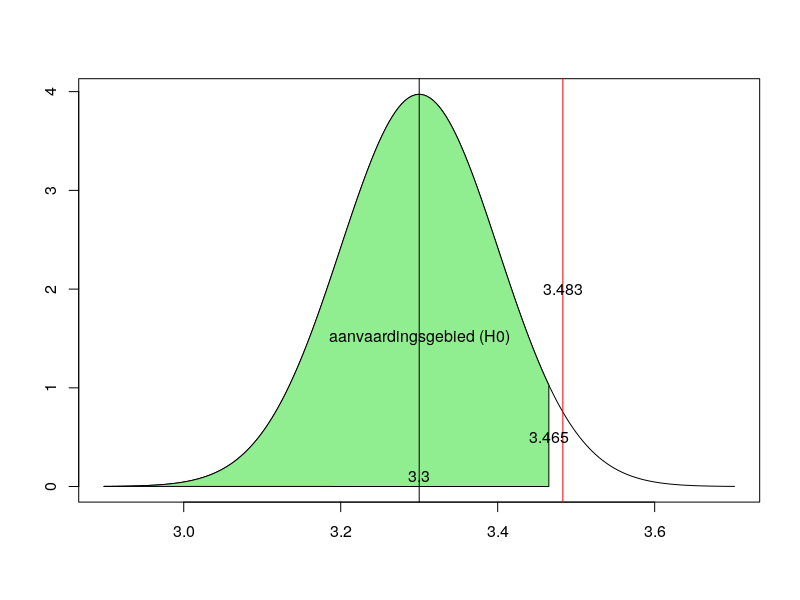
\includegraphics[width=\textwidth]{z-toets-reddingen}
  \caption{Plot in R van de situatie van Voorbeeld~\ref{ex:hypothesetoets-dagelijkse-reddingen}}
\end{figure}

\section{Voorbeelden}

\begin{example}
  Bij een aselecte steekproef van 50 waarnemingen vinden we we volgende grootheden:
  \begin{itemize}
    \item $\overline{x} = 25$
    \item $s = \sqrt{55} = 7,41$
  \end{itemize}
  
  We willen weten of er reden is om aan te nemen dat $\mu$ van de populatie kleiner is dan 27.
  
  \begin{enumerate}
    \item Bepalen van de hypothesen: 
    
    $H_{0} : \mu = 27$ en $H_{1}: \mu < 27$.
    
    \item Vastleggen significantieniveau $\alpha$ en steekproefomvang $n$:
    
    $\alpha = 0,05$ en $n=50$.
    
    \item Waarde toetsingsgrootheid bepalen. 
    
    We kiezen hiervoor het steekproefgemiddelde $M$. Volgens de centrale limietstelling geldt:
    
    \[ M \sim Nor(\mu = 27, \frac{\sigma}{\sqrt{n}}) \]
    De toetsingsgrootheid is
    \[ Z = \frac{\overline{x} - \mu}{\frac{\sigma}{\sqrt{n}}} = \frac{25-27}{\sqrt\frac{55}{50}} \approx -1,91\]
    
    \item Overschrijdingskans berekenen.
    
    We vinden een overschrijdingskans van het gemiddelde van \texttt{pnorm(-1.91)} of ongeveer $0,0281$. Bij een significantieniveau van 0,05 duidt dit er op dat we $H_{0}$ mogen verwerpen.
    
    \item Bereken en teken kritiek gebied.
    
    \[ g = \mu - z \times \frac{\sigma}{\sqrt{n}} \]
    en dus
    
    \[ g = 27 - 1,645 \times \sqrt{\frac{\sigma}{n}} \]
    \[ g =  25,27470944 \]
    
    We vinden dus dat $\overline{x} < g$ komen tot hetzelfde besluit, nl.~dat we $H_{0}$ kunnen verwerpen.
    
  \end{enumerate}
\end{example}

\begin{example}
  In een onderzoek naar het kleingeld dat in de zakken van van onze superhelden zit, stellen de onderzoekers dat zij gemiddeld 25 euro op zak hebben. Ze gaan ervan uit de spreiding $\sigma = 7$ is. Verder zijn de gegevens van de aselecte steekproef van omvang $n=64$ beschikbaar met gemiddeld zakgeld $\overline{x}$ van 23 euro. Voor het significantieniveau kiezen ze $\alpha = 0,05$.
  
  \begin{enumerate}
    \item Bepalen van de hypothesen.
    
    $H_{0} : \mu = 25$ en $H_{1}: \mu \neq 25$.
    
    \item Vastleggen significantieniveau $\alpha$ en steekproefomvang $n$.
    
    $\alpha = 0,05$ en $n=64$.
    
    \item Bepalen van de kritieke grenzen.
    
    \[ g_{1} = \mu - z \times \frac{\sigma}{\sqrt{n}} = 23,28 \]
    
    \[ g_{2} = \mu + z \times \frac{\sigma}{\sqrt{n}} = 26,72 \]
    
    \item Kritiek gebied.
    
    We vinden dat $\overline{x}$ in het kritieke gebied ligt (want $\overline{x} = 23 < g_1 = 23,25$), dus mogen we $H_{0}$ verwerpen.
    
  \end{enumerate}
\end{example}

\section{De \texorpdfstring{$t$}{t}-toets}
\label{sec:t-toets}

Bij de $z$-toets gaan we uit van een aantal veronderstellingen waar we rekening moeten mee houden:

\begin{itemize}
  \item De steekproef moet voldoende groot zijn ($n \ge 30$);
  \item De variatie van de toetsingsgrootheid moet normaal verdeeld zijn;
  \item We veronderstellen dat de standaardafwijking van de populatie, $\sigma$, gekend is.
\end{itemize}

De eerste drie voorwaarden maken dat de centrale limietstelling kan toegepast worden.

Soms zijn deze veronderstellingen niet geldig en mogen we dan ook de $z$-toets \emph{niet} gebruiken! In deze gevallen kunnen we wel gebruik maken van de Student-$t$ verdeling. In de $t$-toets\index{$t$-toets}\index{toets!$t$-} wordt er wel van uit gegaan dat de onderzochte variabele normaal verdeeld is.

De formule voor de kritieke grenswaarde wordt dan aangepast als:

\begin{equation}
g = \mu \pm t \times \frac{s}{\sqrt{n}}
\label{eq:kritieke-waarde-t-toets}
\end{equation}

Voor het bepalen van de $t$-waarde hebben we het aantal vrijheidsgraden nodig, $n-1$. Om de standaardafwijking te schatten, gebruiken we de steekproefstandaardafwijking, $s$.

\begin{example}
  \label{ex:t-toets-dagelijkse-reddingen}
  Stel dat de onderzoekers van de superhelden uit Voorbeeld~\ref{ex:hypothesetoets-dagelijkse-reddingen} door tijdsdruk niet in staat waren om een voldoende grote steekproef te nemen en slechts $n = 20$ observaties gedaan hebben, met hetzelfde steekproefgemiddelde $\overline{x} = 3,483$. De standaardafwijking in deze steekproef bleek $s = 0,55$.
  
  Kunnen we in deze omstandigheden, met eenzelfde significantieniveau $\alpha = 0,05$, het besluit dat superhelden dagelijks \emph{meer} dan 3,3 mensen redden aanhouden?
  
  \begin{enumerate}
    \item Bepalen van de hypothesen.
    
      $H_{0} : \mu = 3,3$ en $H_{1}: \mu > 25$.
    
    \item Vastleggen significantieniveau $\alpha$ en steekproefomvang $n$.
    
    $\alpha = 0,05$ en $n=25$.
    
    \item Bepalen van de kritieke grenswaarde.
    
    \[ g_{2} = \mu + t \times \frac{s}{\sqrt{n}} \approx 3,3 + 1,711 \times \frac{0,55}{\sqrt{25}} \approx 3.488 \]
    
    De waarde voor $t$ wordt in R berekend met \texttt{qt(1-a, df = n - 1)} (met \texttt{a} het significantieniveau en \texttt{df} het aantal vrijheidsgraden.)
    
    \item Conclusie.
    
    We vinden dat $\overline{x} = 3,483$ kleiner is dan de kritieke grenswaarde en dus in het aanvaardingsgebied ligt. Met andere woorden, we mogen $H_{0}$ \emph{niet} verwerpen.
  \end{enumerate}

  Met andere woorden, ook al krijgen we gelijkaardige resultaten in onze steekproef, kunnen we niet hetzelfde besluit trekken. Omdat onze steekproef te klein is, is er grotere onzekerheid of de waarde van het steekproefgemiddelde extreem genoeg is om de nulhypothese te verwerpen.
  
  Hieronder vind je de uitwerking van dit voorbeeld in R.
\end{example}

\lstinputlisting{data/t-toets.R}

\begin{figure}
  \centering
  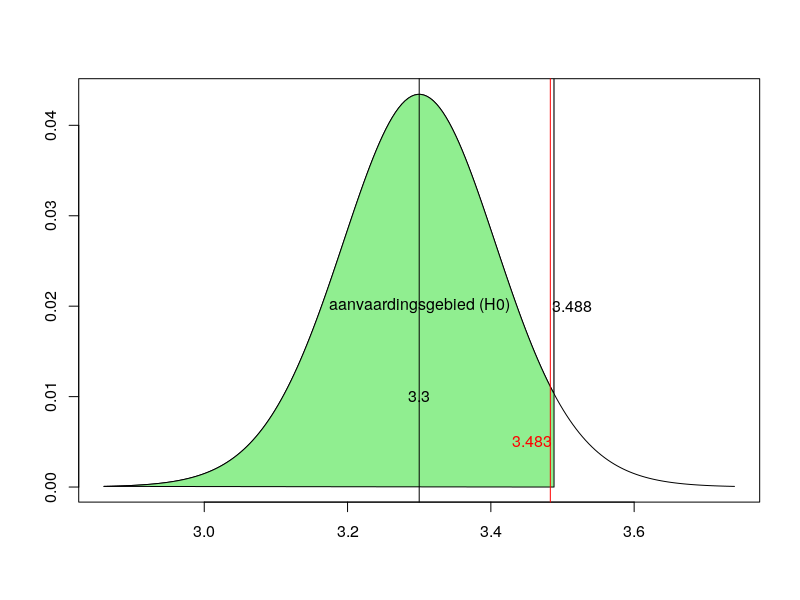
\includegraphics[width=\textwidth]{t-toets-reddingen}
  \caption{Plot in R van de situatie van Voorbeeld~\ref{ex:t-toets-dagelijkse-reddingen}}
\end{figure}

\begin{example}
  Een uitbraak van een door Salmonella veroorzaakte ziekte werd toegeschreven aan vanille-ijs van een bepaalde fabriek~\autocite{Lindquist}. Wetenschappers hebben het niveau van Salmonella gemeten in 9 willekeurig genomen steekproeven.
  
  De niveaus (in MPN/g\footnote{Most Probable Number. Zie bv.~\url{http://www.microbiologie.info/mpn-methode.html} voor meer uitleg over deze methode.}) zijn de volgende:
  
    \begin{center}
    \begin{tabular}{|l|l|l|l|l|}
      \hline
      0,593 & 0,142 & 0,329 & 0,691 & 0,231 \\ \hline
      0,793 & 0,519 & 0,392 & 0,418 &       \\ \hline
    \end{tabular}
  \end{center}

  Is er reden om aan te nemen dat het Salmonella-niveau in het ijs significant groter is dan 0,3 MPN/g? We zullen gebruik maken van de R-functie \texttt{t.test} om deze vraag te beantwoorden. Lees zelf de help-pagina van deze functie om de mogelijke opties te leren kennen.
  
  \begin{enumerate}
    \item Bepalen van de hypothesen
    
    $H_0: \mu = 0.3, H_1: \mu > 0,3$
    
    \item Vastleggen significantieniveau $\alpha = 0.05$ (in R moet je het betrouwbaarheidsniveau $1-\alpha$ opgeven, dus 0,95) en steekproefomvang $n = 9$
    
    \item Bepalen overschrijdingskans. Het gaat hier over een rechtszijdige toets, wat aangegeven wordt met de optie \texttt{alternative="greater"}. Het gekozen betrouwbaarheidsniveau is de standaardwaarde voor deze functie en moet niet expliciet meegegeven worden.
    
\begin{lstlisting}
x <- c(0.593, 0.142, 0.329, 0.691, 0.231, 0.793, 0.519, 0.392, 0.418)
t.test(x, alternative = "greater", mu = 0.3)
\end{lstlisting}
    
    Het resultaat is:
    
\begin{verbatim}
One Sample t-test

data:  x
t = 2.2051, df = 8, p-value = 0.02927
alternative hypothesis: true mean is greater than 0.3
95 percent confidence interval:
0.3245133       Inf
sample estimates:
mean of x 
0.4564444 
\end{verbatim}
    
    \item Conclusie. De overschrijdingskans $p = 0,029 < \alpha = 0,05$. We kunnen dus de nulhypothese verwerpen; er is met ander worden en vrij sterke aanwijzing dat het gemiddelde Salmonella-niveau in het ijs groter is dan 0,3 MPN/g.
    
    Je kan uit de uitvoer van de \texttt{t.test}-functie ook het kritieke gebied aflezen: $[0,3245133; +\infty[$. Het steekproefgemiddelde $0,4564444$ ligt in het kritieke gebied, wat eveneens leidt tot de conclusie dat de nulhypothese kan verworpen worden.
  \end{enumerate}
\end{example}

\section{De \texorpdfstring{$t$}{t}-toets voor twee steekproeven}
\label{sec:t-toets-twee-steekproeven}

De $t$-toets kan ook gebruikt worden om twee steekproeven met elkaar te vergelijken. Je kan er dan mee nagaan of het steekproefgemiddelde van beide steekproeven \emph{significant} verschillend is.

Men maakt onderscheid tussen twee gevallen:

\begin{itemize}
  \item Beide steekproeven zijn onafhankelijk, zijn afzonderlijk genomen. Een voorbeeld is een onderzoek naar een medische behandelingsmethode waar een contolegroep de behandeling \emph{niet} krijgt en een testgroep de behandeling wel krijgt.
  \item De steekproeven zijn afhankelijk, of gepaard. Een voorbeeld is twee metingen uitvoeren op hetzelfde lid van de populatie, zoals de koorts nemen voor en na het innemen van een medicijn om het effect ervan te meten.
\end{itemize}

In R kan je eveneens de functie \texttt{t.test} gebruiken voor het uitvoeren van een toets met twee steekproeven. We geven hieronder twee voorbeelden, één voor elk geval.

\begin{example}
  In een klinisch onderzoek wil men nagaan of een nieuw medicijn als bijwerking een verminderde reactiesnelheid heeft~\autocite{Lindquist}.
  
  Zes deelnemers kregen een medicijn toegekend (interventiegroep) en zes anderen een placebo (controlegroep). Vervolgens werd hun reactietijd op een stimulus gemeten (in ms). We willen nagaan of er significante verschillen zijn tussen de interventie- en controlegroep.
  
  \begin{itemize}
    \item Controlegroep: 91, 87, 99, 77, 88, 91
    \item Interventiegroep: 101, 110, 103, 93, 99, 104
  \end{itemize}
  
  We noteren $\mu_1$ voor het populatiegemiddelde van de patiënten die het medicijn nemen en $\mu_2$ voor het gemiddelde van de niet behandelde populatie.
  
  De hypothesen worden formeel als volgt genoteerd:
  
  $H_0: \mu_1 - \mu_2 = 0$ en $H_1: \mu_1 - \mu_2 < 0$
  
  Het gaat hier dus over een linkszijdige test, wat weergegeven wordt door de optie \texttt{alternative = "less"}. In de nulhypothese veronderstellen we dat het verschil tussen de populatiegemiddelden 0 is, wat met de optie \texttt{mu = 0} wordt aangeduid. Merk op dat dit de standaardwaarde is voor deze parameter en dus in principe niet moet worden opgegeven.
  
\begin{lstlisting}
controle <-  c(91, 87, 99, 77, 88, 91)
interventie <- c(101, 110, 103, 93, 99, 104)
t.test(controle, interventie, alternative="less", mu=0)
\end{lstlisting}

  Het resultaat van de toets:
  
\begin{verbatim}
t.test(controle, interventie, alternative="less")

Welch Two Sample t-test

data:  controle and interventie
t = -3.4456, df = 9.4797, p-value = 0.003391
alternative hypothesis: true difference in means is less than 0
95 percent confidence interval:
-Inf -6.044949
sample estimates:
mean of x mean of y 
88.83333 101.66667
\end{verbatim}

  De $p$ waarde, 0,003391, ligt duidelijk onder het significantieniveau (niet expliciet opgegeven, dus werd de standaardwaarde $\alpha = 0,05$ gebruikt.)
  
  De teststatistiek $t = -3,4456$ ligt binnen het verwerpingsgebied $]-\infty; -6,044949]$.
  
  We mogen dus de nulhypothese verwerpen en besluiten dat volgens de resultaten van deze steekproef het medicijn inderdaad een significant effect heeft op de reactiesnelheid van patiënten.
\end{example}

\begin{example}
  In een studie werd nagegaan of auto's die rijden op benzine met additieven ook een lager verbruik hebben. Tien auto's werden eerst volgetankt met ofwel gewone benzine, ofwel benzine met additieven (bepaald door opgooien van een munt), waarna het verbruik werd gemeten (uitgedrukt in mijl per gallon). Vervolgens werden de auto's opnieuw volgetankt met de andere soort benzine en werd opnieuw het verbruik gemeten. De resultaten worden gegeven in Tabel~\ref{tab:benzineverbruik-additieven}.
  
  \begin{table}
    \centering
    \begin{tabular}{|l|c|c|c|c|c|c|c|c|c|c|}
      \hline 
      Auto & 1 & 2 & 3 & 4 & 5 & 6 & 7 & 8 & 9 & 10 \\ 
      \hline 
      Gewone benzine & 16 & 20 & 21 & 22 & 23 & 22 & 27 & 25 & 27 & 28 \\ 
      \hline 
      Additieven & 19 & 22 & 24 & 24 & 25 & 25 & 25 & 26 & 28 & 32 \\ 
      \hline 
    \end{tabular} 
  \caption{Verbruik in mijl per gallon met 2 soorten benzine.}
  \label{tab:benzineverbruik-additieven}
  \end{table}
  
  We gaan door middel van een \emph{gepaarde $t$-test} na of auto's significant zuiniger rijden met benzine met additieven.
  
  De optie \texttt{paired=TRUE} geeft aan dat het hier om een gepaarde $t$-toets gaat.
  
\begin{lstlisting}
gewone    <- c(16, 20, 21, 22, 23, 22, 27, 25, 27, 28)
additieven <-c(19, 22, 24, 24, 25, 25, 26, 26, 28, 32)
t.test(additieven, gewone, alternative="greater", paired=TRUE)
\end{lstlisting}

  Resultaat:
  
\begin{verbatim}
 Paired t-test

data:  additieven and gewone
t = 4.4721, df = 9, p-value = 0.0007749
alternative hypothesis: true difference in means is greater than 0
95 percent confidence interval:
 1.180207      Inf
sample estimates:
mean of the differences 
                      2 
\end{verbatim}

  De $p$-waarde, 0,0007749, ligt onder het significantieniveau, dus we kunnen de nulhypothese verwerpen. Volgens deze steekproef rijden auto's inderdaad zuiniger met benzine met additieven.
  
  De teststatistiek $t = 4,4721$ ligt binnen het verwerpingsgebied $[1,180207; +\infty]$.
\end{example}

% TODO: later evt. toevoegen
% - ANOVA, variantie-analyse
% - Kolmogorov-Smirnov test

\section{Fouten in hypothesetoetsen}

Bij het uitvoeren van een hypothesetoets kunnen altijd nog fouten optreden. Indien we $H_{0}$ verwerpen wanneer ze in werkelijkheid juist is, spreken we van een fout van type I en wanneer we $H_{0}$ ten onrechte aanvaarden van een fout van type II.

Het significatieniveau $\alpha$ bepaalt bij het uitvoeren van een hypothesetoets wanneer de nulhypothese precies verworpen kan worden. Stel dat we een significatieniveau van 5\% kiezen. Als de nulhypothese waar is, dan is de kans dat we een steekproef trekken met een toetsingswaarde die in het verwerpingsgebied terecht komt 5\%. M.a.w. de kans om de nulhypothese te verwerpen terwijl ze waar is, is 5 \% of in het algemeen: het significantieniveau van een toets is gelijk aan de kans op het maken van een fout van type I.

Het is vanzelfsprekend dat we de kans op een fout van type I zo klein mogelijk willen houden. Jammer genoeg is dit ten koste van de kans op een type II fout, aangeduid met $\beta$, die hierdoor groter wordt. Het verband tussen $\alpha$ en $\beta$ is niet triviaal en we gaan hier in deze cursus niet verder op in.

In vele gevallen is het maken van een fout van type I erger dan een van type II. Denk maar aan een rechtszaak waarbij de nulhypothese is dat de persoon onschuldig is. Indien we toetsen op een 5\% significantieniveau is de kans op een type I fout 5 op 100. M.a.w. er is een betrouwbaarheid van 95\% dat de juiste beslissing wordt genomen indien $H_{0}$ correct is. Daarom vermijden we liever de conclusie dat $H_{0}$ geaccepteerd wordt, maar eerder dat de steekproef onvoldoende bewijs bevat om $H_{0}$ bij een bepaald significantieniveau te verwerpen.

\begin{table}
  \centering
  \begin{tabular}{@{}l|cc@{}}
    \toprule
    & \multicolumn{2}{c}{\textbf{Werkelijke stand van zaken}} \\
    \textbf{Conclusies}          & \textbf{$H_{0}$ correct} & \textbf{$H_{1}$ correct}     \\
    \midrule
    \textbf{$H_{0}$ geaccepteerd}& Juist                    & Fout van type II \\
    \textbf{$H_{0}$ verworpen}   & Fout van type I          & Juist            \\
    \bottomrule
  \end{tabular}
  \caption{Conclusies en consequenties bij toetsen van een hypothese; types van fouten.}
  \label{tab:hypfouten}
\end{table}

\section{Oefeningen}
\label{sec:toetsingsprocedures-oefeningen}

\begin{exercise}
  Betrouwbaarheidsintervallen.
  
  \begin{enumerate}
    \item Wat is de onder- en bovengrens van een betrouwbaarheidsinterval van 99\%?
    \item Een betrouwbaarheidsinterval van 99\% is breder dan een van 95\%. Waarom is dit zo?
    \item Hoe zou het betrouwbaarheidsinterval voor 100\% er uit zien?
  \end{enumerate}
  
\end{exercise}

\begin{exercise}
  \label{oef:bindend-studieadvies}
  
  Er wordt gezegd dat het invoeren van een bindend studieadvies (BSA) een rendementsverhoging tot gevolg heeft in slaagkans. Voor het invoeren van het BSA was in de studentenpopulatie het gemiddelde aantal behaalde studiepunten per jaar per student gelijk aan 44 met een standaardafwijking van 6,2. Na invoering van het BSA wijst een onderzoek uit onder 72 studenten dat deze een gemiddeld aantal studiepunten haalden van 46,2.
  
  \begin{enumerate}
    \item Toets of er bewijs is dat het invoeren van een BSA leidt tot een rendementsverhoging. Gebruik methode van kritieke grenswaarde. ($\sigma = 6,2, \alpha = 2,5\%$).
    \item Toon hetzelfde aan met de methode van de overschrijdingskans.
    \item Geef een interpretatie wat de betekenis is van $\alpha = 2,5 \%$.
  \end{enumerate}
\end{exercise}

\begin{exercise}
  \label{oef:prijsverschil-autos}
  
  Eén van de motieven voor het kiezen van een garage is de inruilprijs voor de oude auto. De importeur van Ford wil graag dat de verschillende dealers een gelijk prijsbeleid voeren. De importeur vindt dat het gemiddelde prijsverschil tussen de dichtstbijzijnde Ford-dealer en de dealer waar men de auto gekocht heeft hoogstens \euro{300} mag bedragen. De veronderstelling is dat als het verschil groter is, potentiële klanten eerder geneigd zullen zijn om bij hun vorige dealer te blijven.
  
  In een steekproef worden volgende verschillen genoteerd:
  
  \begin{center}
    \begin{tabular}{|l|l|l|l|l|l|l|}
      \hline
      400 & 350 & 400 & 500 & 300 & 350 & 200 \\ \hline
      500 & 200 & 250 & 250 & 500 & 350 & 100 \\ \hline
    \end{tabular}
  \end{center}

  Toets of er reden is om aan te nemen dat het gemiddelde prijsverschil in werkelijkheid significant groter is dan \euro{300}. Gebruik een significantieniveau van 5\%. 
  
\end{exercise}

\begin{exercise}
  \label{oef:casus-akin2016-toets}
  
  In Oefening~\ref{oef:casus-akin2016-1var} en volgende hebben we de resultaten van performantiemetingen voor persistentiemogelijkheden in Android geanalyseerd~\autocite{Akin2016}. Er werden experimenten uitgevoerd voor verschillende combinaties van hoeveelheid data (klein, gemiddeld, groot) en persistentietype (GreenDAO, Realm, SharedPreferences, SQLite). Voor elke hoeveelheid data hebben we kunnen bepalen welk persistentietype het beste resultaat gaf.
  
  Nu gaan we uitzoeken of het op het eerste zicht beste persistentietype ook \emph{significant} beter is dan de concurrentie.
  
  Concreet: ga aan de hand van een toets voor twee steekproeven voor elke datahoeveelheid na of het gemiddelde van het best scorende persistentietype \emph{significant lager} is dan het gemiddelde van \begin{inparaenum}[(i)] \item het \emph{tweede} beste en \item het slechtst scorende type \end{inparaenum}.
  
  Kunnen we de conclusie aanhouden dat voor een gegeven datahoeveelheid één persistentietype het beste is, d.w.z.~significant beter is dan gelijk welk ander persistentietype?
\end{exercise}

\begin{exercise}
  Een groot aantal studenten heeft deelgenomen aan een test die in verschillende opeenvolgende sessies werd georganiseerd. Omdat het opstellen van een aparte opgave voor elke sessie praktisch onhaalbaar was, is telkens dezelfde opgave gebruikt. Eigenlijk bestaat er dus het gevaar dat studenten na hun sessie info konden doorspelen aan de groepen die nog moesten komen. De latere groepen hebben dan een voordeel ten opzichte van de eerste. Blijkt dit ook uit de cijfers?
  
  Het bestand \texttt{puntenlijst.csv} bevat alle resultaten van de test. Elke groep wordt aangeduid met een letter, in de volgorde van de sessie.
  
  \begin{itemize}
    \item Dag 1: sessies A, B
    \item Dag 2: sessies C, D, E
    \item Dag 3: sessies F, G, H
  \end{itemize}

  Sessies A en B zijn doorgegaan op een andere campus, dus er zou kunnen verondersteld worden dat er weinig tot geen communicatie is met de studenten van de andere sessies.
  
  Als er info met succes doorgespeeld werd, dan verwachten we dat de scores van de groepen die later komen significant beter zijn dan de eerste.
  
  Merk op dat de omgekeerde redenering niet noodzakelijk geldt: als blijkt dat het resultaat van de latere sessies inderdaad significant beter blijkt, dan betekent dat niet noodzakelijk dat de oorzaak (enkel) het doorspelen van informatie is. Er kunnen ook andere oorzaken zijn (bv.~``zwakkere'' klasgroepen zijn toevallig eerder geroosterd).
  
  \begin{enumerate}
    \item Ga op verkenning in de data. Bereken de gepaste centrum- en spreidingsmaten voor de dataset als geheel en voor elke sessie afzonderlijk.
    
    \item Maak een staafgrafiek van de gemiddelde score per sessie. Is dit voldoende om een beeld te vormen van de resultaten? Waarom (niet)?
    
    \item Maak een boxplot van de scores opgedeeld per groep. Vergelijk onderling de hieronder opgesomde sessies. Denk je dat er een significant verschil is tussen de resultaten? Wordt ons vermoeden dat er informatie doorgespeeld wordt bevestigd?
    
    \begin{itemize}
      \item A en B
      \item C, D en E
      \item F, G en H
      \item C en H
      \item A en H
    \end{itemize}
  
    \item Ga door middel van een geschikte statistische toets voor na of de verschillen tussen die hierboven opgesomde groepen ook \emph{significant} is. Kunnen we concluderen dat de latere groepen beter scoren of niet?
  \end{enumerate}
\end{exercise}

\section{Antwoorden op geselecteerde oefeningen}
\label{sec:toetsingsprocedures-antwoorden}

\paragraph{Oefening~\ref{ex:kritieke-waarde-linkszijdig}:}

\begin{equation}
g = \mu - z \times \frac{\sigma}{\sqrt{n}}
\label{eq:kritiekeRechtseWaarde2}
\end{equation}

want

\[ P(M < g) = P\left(Z < \frac{g - \mu}{\frac{\sigma}{\sqrt{n}}}\right) = 0,05 \]
Wegens de symmetrieregel kunnen we zeggen
\[ P\left(Z > - \left( \frac{g - \mu}{\frac{\sigma}{\sqrt{n}}} \right) \right) = 0,05 \]
De z-waarde die ermee overeen komt is 1,645 dus hebben we
\[ z = \frac{-g + \mu}{\frac{\sigma}{\sqrt{n}}} \]
\[ \Leftrightarrow -g = \frac{\sigma}{\sqrt{n}} z - \mu \]
\[ \Leftrightarrow g = -\frac{\sigma}{\sqrt{n}} z + \mu \]

\paragraph{Oefening~\ref{oef:bindend-studieadvies}}

\begin{enumerate}
  \item $g \approx 45,4 < \overline{x} = 46,2$.
  
  $\overline{x}$ ligt in het kritieke gebied, dus we mogen de nulhypothese verwerpen. We hebben dus redenen om aan te nemen dat bindend studieadvies inderdaad het studierendement significant verhoogt.
  
  \item $P(M > 46.2) \approx 0,0013 < \alpha = 0,025$. De overschrijdingskans is kleiner dan het significantieniveau, dus we mogen de nulhypothese verwerpen.
  
  \item  $\alpha$ is de kans dat je $H_{0}$ ten onrechte verwerpt. Er is m.a.w.~een kans van 2,5\% dat je ten onrechte de conclusie trekt dat het studierendement hoger is geworden.
\end{enumerate}

\paragraph{Oefening~\ref{oef:prijsverschil-autos}}

In deze situatie ($n = 14 < 30$) mogen we geen $z$-toets gebruiken, maar vallen we terug op de $t$-toets.

\begin{itemize}
  \item $\overline{x} \approx 332,143$
  \item $s \approx 123,424$
  \item $g \approx 358,42$. Het steekproefgemiddelde ligt niet in het kritieke gebied, dus we kunnen $H_0$ \emph{niet} verwerpen.
  \item $p \approx 0,1738$. $p \nless \alpha$, dus we kunnen $H_0$ \emph{niet} verwerpen.
\end{itemize}

Er is op basis van deze steekproef dus geen reden om aan te nemen dat het gemiddelde prijsverschil op de inruilprijs van oude wagens significant groter is dan door de importeur aanbevolen.

\paragraph{Oefening~\ref{oef:casus-akin2016-toets}}

Tabel~\ref{tab:akin2016-resultaten-ttoets} geeft een overzicht met voor elke datasetgrootte het beste en tweede beste persistentietype (op basis van het steekproefgemiddelde). De conclusie van~\textcite{Akin2016}, dat \emph{Realm} het performantste persistentietype is, blijft overeind, maar voor de kleine datasets is het verschil niet significant.

Merk op dat we hier niet expliciet vooraf een significantieniveau gekozen hebben. Voor $\alpha = 0,1$, $0,5$ of zelfs $0,01$, kunnen we echter dezelfde conclusie trekken.

\begin{table}
  \begin{center}
\begin{tabular}{llll}
  \toprule
  \textbf{Grootte} & \textbf{Beste} & \textbf{2e beste} & \textbf{$p$-waarde} \\ \midrule
  Small            & Realm          & SharedPreferences & 0.1699     \\
  Medium           & Realm          & GreenDAO          & 0.0002506  \\
  Large            & Realm          & SQLite            & 0.0017     \\ \bottomrule
\end{tabular}
\end{center}
  \caption{Resultaten $t$-toets voor de beste en 2e beste persistentietype op basis van steekproefgemiddelde~\autocite{Akin2016}.}
  \label{tab:akin2016-resultaten-ttoets}
\end{table}
\chapter{Analyse op 2 variabelen}
\label{ch:analyse2var}

In de vorige hoofdstukken hebben we telkens één variabele tegelijkertijd onderzocht. Vaak hebben onderzoeksvragen echter te maken met \emph{verbanden} (en dan vooral oorzakelijke) tussen variabelen. In dit hoofstuk gaan we hier verder op in.

Wanneer we een verband beschrijven tussen variabelen, onderscheiden we:

\begin{itemize}
  \item De \emph{afhankelijke variabele}\index{variabele!afhankelijke}, waarover we een voorspelling willen doen;
  \item De \emph{onafhankelijke variabele}\index{variabele!onafhankelijke}, op basis van dewelke we de voorspelling doen.
\end{itemize}

Als de onafhankelijke variabele op een bepaalde manier verandert, verwachten we dat de waarde van de afhankelijke variabele op een voorspelbare manier mee verandert.

\begin{example}
  Een voorbeeld waarbij verbanden kunnen gevonden tussen variabelen vind je bijvoorbeeld bij Ant Colony Optimization (ACO). Dit is een techniek die gebruikt wordt in verschillende computationele problemen. Men baseert zich hier op hoe mieren voedsel zoeken en  vinden en dat communiceren aan de groep. Mieren verspreiden feromonen als ze op pad gaan op zoek naar eten. Hoe langer het pad, hoe minder feromonen het pad zal bevatten, hoe korter het pad, hoe groter de kans dat er een grote concentratie aan feromonen te vinden is. Mieren worden aangetrokken door deze feromonen en zullen dus proberen de meest bewandelde paden te gebruiken om naar een bepaalde voedselbron te gaan. Nu kan je onderzoeken of de tijd voor het vinden van een pad, afhangt van een aantal variabelen:

  \begin{itemize}
    \item De mate waarin feromonen verspreid worden
    \item De mate waarin een feromoon verdwijnt
    \item Het aantal obstakels tussen het nest en de voedselbron
    \item De vorm van de obstakels tussen nest en voedselbron (vinden ze sneller het pad indien er geen hoeken aan de obstakels zijn bv.)
  \end{itemize}
\end{example}

Om een vergelijking te maken kunnen we \begin{inparaenum}[(i)]
\item de bekende statistieken zoals gemiddelde e.a. berekenen en analyseren of \item grafische voorstellingen maken van deze statistieken. \end{inparaenum}

Welke soort van grafieken we kunnen gebruiken hangt af van het meetniveau:
@
\begin{itemize}
  \item Interval of ratio:

    \begin{itemize}
      \item Staafdiagram van de gemiddelden
      \item Boxplot per groep
    \end{itemize}
  \item Ordinaal of nominaal

    \begin{itemize}
      \item Kruistabel
      \item Geclusterd staafdiagram
      \item Rependiagram
    \end{itemize}
\end{itemize}

Bij de vraag of er samenhang is tussen twee variabelen kunnen we volgende grafieken/statistieken gebruiken:

\begin{itemize}
  \item Nominaal x Nominaal:

    \begin{itemize}
      \item Kruistabel met Cramér's V
    \end{itemize}
  \item Ordinaal x Ordinaal
    \begin{itemize}
      \item Geclusterd staafdiagram
      \item Rependiagram
    \end{itemize}
  \item Ratio x Ratio

    \begin{itemize}
      \item Spreidingsdiagram
      \item Regressie en correlatie met correlatiecoëfficiënt.
    \end{itemize}
\end{itemize}

\section{Kruistabellen en Cramér's V}

\begin{definition}[Kruistabel]
  In een kruistabel\index{kruistabel} (zie bv.~Figuur~\ref{tab:kruistabel0}) worden de frequenties van twee variabelen samengevat.
  
  Elke cel van de laatste kolom bevat de som van de overeenkomstige rij en elke cel van de laatste rij bevat de som van de overeenkomstige kolom. Dit worden de \emph{marginale totalen}\index{totaal!marginaal}\index{marginaal totaal} genoemd.
\end{definition}

In R kan je een kruistabel (Eng.: \emph{contingency table} of \emph{cross table}) opstellen met de functie \texttt{table}. Een voorbeeld i.v.m.~de oefening over Android persistentietypes (zie Oefening~\ref{oef:casus-akin2016-1var}):

\begin{lstlisting}
> table(Datahoeveelheid, PeristentieType)
        PersistentieType
DataHoeveelheid GreenDAO Realm Sharedpreferences SQLLite
Large                 30    30                 0      30
Medium                30    30                 0      30
Small                 30    30                30      30
\end{lstlisting}

\begin{table} \centering
  \begin{tabular}{@{}rrrr}
    \toprule
                & Vrouw & Man & Totaal \\ \midrule
           Goed &     9 &   8 &     17 \\
      Voldoende &     8 &  10 &     18 \\
    Onvoldoende &     5 &   5 &     10 \\
         Slecht &     0 &   4 &      4 \\
         Totaal &    22 &  27 &     49 \\ \bottomrule
  \end{tabular}
  \caption{Een kruistabel voor de waardering door mannen en vrouwen van een bepaald assortiment producten.}
  \label{tab:kruistabel0}
\end{table}

In een gewone kruistabel kunnen we geen directe conclusies trekken, aangezien het analyseren of er samenhang bestaat tussen variabelen niet goed gaat op basis van de celfrequenties. Niet alle metingen zijn even groot! Daarom moeten we percenteren. Nog even snel de regel van percenteren:

\begin{itemize}
  \item Om te weten hoeveel percent $x$ is van $y$, deel je $x$ door $y$ en vermenigvuldig je met 100: $perc = 100 \times \frac{x}{y}$.
  \item Om te weten hoeveel $x$ \% is van $y$ : $ \frac{x \times y}{100}$
\end{itemize}

\begin{example}
  \label{vb:kruistabel}
  In Tabel~\ref{tab:kruistabel0} vinden we de data waar er gekeken wordt naar het verschil in waardering van een assortiment tussen mannen en vrouwen. We percenteren per geslacht en vinden bijvoorbeeld dat 41\% van de vrouwen een waardering goed heeft (zie Tabel~\ref{tab:kruistabel1}). Nu kunnen we ons de vraag stellen of de waarderingskeuze afhangt van het geslacht van de persoon.
\end{example}

In ons voorbeeld kunnen we besluiten dat 30\% van de mannen tevreden is en 15\% van de mannen ontevreden. Maar hoe goed is die samenhang tussen de verschillende variabelen (geslacht en tevredenheid)? Dat kunnen we bepalen aan de hand van Cramér's V. Voordat we die definitie kunnen geven, moeten we echter eerst de waarde $\chi^2$ introduceren.

\begin{table} \centering
  \begin{tabular}{@{}rrrrrrr@{}} \toprule
    & Vrouw & Man & Totaal & Vrouw \% & Man\%   & Totaal  \\ \midrule
    Goed        & 9     & 8   & 17     & 41\%  & 30\% & 35\% \\
    Voldoende   & 8     & 10  & 18     & 36\%  & 37\%    & 37\% \\
    Onvoldoende & 5     & 5   & 10     & 23\%  & 18\% & 20\% \\
    Slecht      & 0     & 4   & 4      & 0\%      & 15\% & 8\%  \\
    Totaal      & 22    & 27  & 49     & 100\%    & 100\%   & 100\%   \\
    \bottomrule
  \end{tabular}
  \caption{De kruistabel waarbij we de waarden gepercenteerd hebben.}
  \label{tab:kruistabel1}
\end{table}

\section{\texorpdfstring{$\chi^{2}$}{chi-kwadraat} test voor associatie}
\index{$\chi^{2}$waarde}

De $\chi^{2}$ (\emph{chi-kwadraat}) waarde is een grootheid die gebruikt wordt om te bepalen of er een significant verband bestaat tussen twee variabelen. Meer hierover volgt later in Hoofdstuk~\ref{ch:chikwadraat}. De berekening ervan leggen we alvast hier uit.

\begin{enumerate}
  \item Stel de kruistabel op samen met marginale totalen (zie tabel \ref{tab:kruistabel1}).
  \item Stel voor elke cel een schatter op voor de theoretische kans om in die cel te geraken. Deze schatter kan je bereken als volgt: (kans op in de rij van deze cel te komen) $\times$ (kans om in de kolom van de cel te komen). In het voorbeeld is dit dus voor cel$_{1,2}$:
  
  \[P[rij_{1}] \times P[kolom_{2}] = \frac{17}{49} \times \frac{27}{49} = 0.191170346 \]
  Algemeen kan je dus stellen dat de verwachte theoretische waarde $e$ als volgt kan berekend worden:

  \begin{equation}
    e = (\frac{rijtotaal}{n} \times \frac{kolomtotaal}{n}) \times n = \frac{rijtotaal \times kolomtotaal}{n}
  \end{equation}

  Met:

  \begin{itemize}
    \item $e$ verwachte waarde bij onafhankelijkheid
    \item $rijtotaal$ totaal van de rij van de betreffende cel
    \item $kolomtotaal$ totaal van de kolom van de betreffende cel
  \end{itemize}

  Voor cel$_{1,2}$ is dit dus 9.36.
  
  \item Dan bereken je het verschil tussen geobserveerde (notatie $a$) en verwachte frequentie ($e$). (Zie tabel \ref{tab:kruistabel2})
  
  \item De laatste stap houdt in dat we een berekening gaan maken voor de maat van afwijking voor elke cel. Opnieuw gaan we hier een kwadraat nemen om het teken kwijt te spelen. We gaan ook de afwijking delen door de verwachte theoretische waarde om hen relatief even belangrijk te maken. Bijvoorbeeld: een afwijking van 5 op een verwachte frequentie van 20 is groter dan bv. een afwijking op een verwachte waarde van 200. Dit geeft dan volgende berekening (zie Tabel~\ref{tab:kruistabel3}):
  
  \begin{equation}
    \frac{(a-e)^{2}}{e}
  \end{equation}
  
  \item Deze gekwadrateerde deviaties gaan we dan optellen en vormt de $\chi^{2}$ \footnote{Let op dat er afgerond wordt.}
  
  \begin{equation}
    \chi^{2} = \sum \frac{(a-e)^{2}}{e}
  \end{equation}
\end{enumerate}

\begin{table} \centering
  \begin{tabular}{@{}rrrrrrr@{}} \toprule
    & Vrouw & Man & Totaal & Vrouw \% & Man\%   & Totaal  \\ \midrule
    Goed        & $9 -\textcolor{red}{7.63}$     & $8 - \textcolor{red}{9.36}$   & $17$     & $41$\%  & $30$\% & $35$\% \\
    Voldoende   & $8 - \textcolor{red}{8.08}$   & $10 - \textcolor{red}{9.91}$  & $18$     & $36$\%  & $37$\%    & $37$\% \\
    Onvoldoende & $5 - \textcolor{red}{4.48}$    & $5 - \textcolor{red}{5.51}$  & $10$     & $23$\%  & $18$\% & $20$\% \\
    Slecht      & $0 - \textcolor{red}{1.79}$    & $4 - \textcolor{red}{2.20}$  & $4$      & $0$\%      & $15$\% & $8$\%  \\
    Totaal      & $22$    & $27$  & $49$     & $100$\%    & $100$\%   & $100$\%   \\
    \bottomrule
  \end{tabular}
  \caption{De kruistabel waarbij we de schatter $e$  (hetgeen we verwachten bij geen samenhang) bepaald hebben voor elke cel en die aftrekken van de geobserveerde waarde.}
  \label{tab:kruistabel2}
\end{table}

\begin{table} \centering
  \begin{tabular}{@{}rrrrrrr@{}} \toprule
    & Vrouw                   & Man                     & Totaal & Vrouw \% & Man\%   & Totaal  \\ \midrule
    Goed        & $\textcolor{blue}{0.2}$ & $\textcolor{blue}{0.2}$ & $17$   & $41$\%   & $30$\%  & $35$\% \\
    Voldoende   & $\textcolor{blue}{0}$   & $\textcolor{blue}{0}$   & $18$   & $36$\%   & $37$\%  & $37$\% \\
    Onvoldoende & $\textcolor{blue}{0.1}$ & $\textcolor{blue}{0}$   & $10$   & $23$\%   & $18$\%  & $20$\% \\
    Slecht      & $\textcolor{blue}{1.8}$ & $\textcolor{blue}{1.5}$ & $4$    & $0$\%    & $15$\%  & $8$\%  \\
    Totaal      & $22$                    & $27$                    & $49$   & $100$\%  & $100$\% & $100$\%   \\
    \bottomrule
  \end{tabular}
  \caption{De kruistabel waarbij we het verschil gekwadrateerd en genormeerd hebben.}
  \label{tab:kruistabel3}
\end{table}

Met deze statistiek kunnen de waarde Cramér's V\index{Cramér's V} berekenen:

\begin{definition}[Cramér's V]
  \begin{equation}
    V = \sqrt{\frac{\chi^{2}}{n(k-1)}}
    \label{eq:Craemer}
  \end{equation}
  met
  \begin{itemize}
    \item $\chi^{2}$ de berekende chi-kwadraatwaarde.
    \item $n$ het aantal waarnemingen.
    \item $k$ = de kleinste waarde van het aantal kolommen of het aantal rijen van de tabel.
  \end{itemize}

\end{definition}

Cramér's V is de $\chi^{2}$, gecorrigeerd voor steekproefomvang en het aantal categorieën in de variabelen. Het resultaat is altijd een getal tussen 0 en 1. Tabel~\ref{tab:interpretatie-cramers-v} geeft aan hoe je het resultaat kan interpreteren.

\begin{table}
  \centering
  \begin{tabular}{ll}
    $V = 0$ & geen samenhang \\
    $V \approx 0,1$ & zwakke samenhang \\
    $V \approx 0,25$ & redelijk sterke samenhang \\
    $V \approx 0,50$ & sterke samenhang \\
    $V \approx 0,75$ & zeer sterke samenhang \\
    $V = 1$ & volledige samenhang \\
  \end{tabular}
  \caption{Interpretatie van de waarde van Cramérs'V}
  \label{tab:interpretatie-cramers-v}
\end{table}

Voor ons voorbeeld waarbij gekeken wordt naar de samenhang tussen geslacht en waardering van het assortiment vinden we een $\chi^{2}= 3.811$ en dus een Cramér's V van $0.279$ (want $n = 49$ en $k = 2$), wat duidt op redelijk sterke samenhang tussen de variabelen. Met andere woorden, de resultaten van de bevraging geven aan dat er een verschil is in de waardering die vrouwen en mannen geven over het assortiment.

Hieronder vind je de uitwerking van Voorbeeld~\ref{vb:kruistabel} in R.

\lstinputlisting{data/kruistabellen.R}

\begin{example}
  In Tabel~\ref{tab:autovoorkeur} worden de voorkeuren van vrouwen en mannen voor de gegeven automerken opgesomd. We zien dat nog steeds dertig van de honderd respondenten een voorkeur hebben voor de Mercedes, maar dat tweederde van deze dertig vrouwen zijn. We zouden  ook kunnen zeggen dat de helft van de vrouwen een voorkeur heeft voor de Mercedes. Evenzo blijkt dat een derde van de mannen een voorkeur heeft voor een Alfa Romeo, tegenover geen van de vrouwen. Het lijkt alsof de onderscheiden automerken niet gelijkelijk gewaardeerd worden door mannen en vrouwen. Om dit te staven bepalen we $\chi^{2}$ en Cramér's V. Probeer dit zelf, hetzij in R, hetzij met een rekenblad (Excel, Numbers, LibreOffice Calc)! We vinden:
  \[ \chi^{2} = 22.619 \]
  \[ V = \sqrt{\frac{22.169}{100 . (2-1)}}  = 0.476\]

  We vinden dus tussen een sterke tot zeer sterke samenhang.
\end{example}

\begin{table} \centering
  \begin{tabular}{@{}rrrrrr@{}}
  	\toprule
  	        & Mercedes &  BMW & Porsche & Alfa Romeo & Totaal \\ \midrule
  	 Mannen &     $10$ & $10$ &    $20$ &       $20$ &   $60$ \\
  	Vrouwen &     $20$ &  $5$ &    $15$ &        $0$ &   $40$ \\
  	 Totaal &     $30$ & $15$ &    $35$ &       $20$ &  $100$ \\ \bottomrule
  \end{tabular}
  \caption{Tabel die uitdrukt hoeveel vrouwen en hoeveel mannen een voorkeur voor een bepaald automerk hebben.}
  \label{tab:autovoorkeur}
\end{table}

\section{Regressie}
\label{sec:regressie}

Bij \index{Regressie} regressie gaan we proberen een consistente en systematische koppeling tussen de variabelen te vinden. Dat betekent concreet: ``als we de waarde van de onafhankelijke variabele kennen, kunnen we dan ook de waarde van de afhankelijke variabele voorspellen?'' We kennen twee soorten verbanden:
\begin{description}
  \item [Monotoon:] een monotoon verband is een verband waarbij de onderzoeker de algemene richting van de samenhang tussen de twee variabelen kan aanduiden, hetzij stijgend, hetzij dalend. De richting van het verband verandert nooit.
  \item [Niet-monotoon:] bij een niet-monotoon verband wordt de aanwezigheid (of afwezigheid) van de ene variabele systematisch gerelateerd aan de aanwezigheid (of afwezigheid) van een andere variabele. De richting van het verband kan echter niet aangeduid worden.
\end{description}

Bij lineaire regressie gaan we ons beperken tot een lineair verband: een rechtlijnige samenhang tussen een onafhankelijke en afhankelijke variabele, waarbij kennis van de onafhankelijke variabele kennis over de afhankelijke variabele geeft.

Bij een lineair verband zijn er drie karakteristieken:

\begin{enumerate}
  \item Aanwezigheid: is er wel een verband tussen de twee variabelen?
  \item Richting: is er een dalend of een stijgend verband?
  \item Wat is de sterkte van het verband: sterk, gematigd of niet-bestaand?
\end{enumerate}

Een voorbeeld van een linear verband $y = \beta_{0} + \beta_{1}x$  vind je bijvoorbeeld in figuur \ref{fig:regressieFig}.

\begin{figure}[t]
  \begin{tikzpicture}
    \begin{axis}[
        axis x line=middle,
        axis y line=middle,
        enlarge y limits=true,
        width=\textwidth, height=8cm,     % size of the image
        grid = major,
        grid style={dashed, gray!30},
        ylabel=$y$,
        xlabel=$x$,
        legend style={at={(0.1,-0.1)}, anchor=north}
      ]
      \addplot[only marks] table  {data/regressie.dat};
      \addplot [no markers, thick, red] table [y={create col/linear regression={y=y}}] {data/regressie.dat};
    \end{axis}
  \end{tikzpicture}
  \caption{Een voorbeeld van een lineair verband}
  \label{fig:regressieFig}
\end{figure}

Zo'n verband kunnen we vinden aan de hand van de \index{Kleinste kwadraten methode} kleinste kwadraten methode van Gauss. Dit wordt als volgt gedaan.

\begin{theorem}

  Een lineair verband wordt weergegeven als volgt:

  \begin{equation}
    y = \beta_{0} + \beta_{1} x
    \label{eq:lineair}
  \end{equation}
  met
  \begin{itemize}
    \item $y$ de afhankelijke
    \item $x$ de onafhankelijke
  \end{itemize}

  We willen hier de som van de kwadraten minimaliseren van de afwijkingen $e_{i} = y_{i} - (\beta_{0} + \beta_{1}x_{i})$. Zo'n afwijking kan ook geschreven worden als (stel $X_{i} = x_{i} - \overline{x}$ en $Y_{i} = y_{i} - \overline{y}$):

  \begin{eqnarray}
    e_{i} & = & y_{i} - \beta_{1} x_{i} - \beta_{0} \\
    e_{i} & = & (y_{i} - \overline{y}) - \beta_{1}(x_{i} - \overline{x}) - (\beta_{0} - \overline{y} + \beta_{1} \overline{x}) \\
    \label{eq:regressie-bewijs}
    e_{i} & = & Y_{i} - \beta_{1} X_{i} - (\beta_{0} - \overline{y} + \beta_{1} \overline{x})
  \end{eqnarray}

  In stap~\ref{eq:regressie-bewijs} doen we eigenlijk $+\overline{x}-\overline{x}+\overline{y}-\overline{y}$, wat een nuloperatie is. Dit is een gedachtensprong die niet meteen voor de hand ligt, maar onthou dat dit een ``shortcut'' is naar de oplossing en dat het ``echte'' bewijs een stuk ingewikkelder is.

  We willen de som van de kwadraten van $e_i$  minimaliseren:

  \begin{eqnarray}
    \sum_{i}^{n} e_{i}^{2} & =& \sum_{i}^{n} (y_{i} - (\beta_{0} + \beta_{1}x_{i}))^{2}\\
    & = & \sum_{i}^{n} ((Y_{i} - \beta_{1} X_{i}) - (\beta_{0} - \overline{y} + \beta_{1}\overline{x}))^{2}\\
    & = & \sum_{i}^{n}(Y_{i} - \beta_{1} X_{i})^2 - 2 \sum_{i}^{n}(Y_i - \beta_1 X_i)(\beta_0 - \overline{y})+ \beta_1\overline{x}) + (\beta_{0} - \overline{y} + \beta_{1}\overline{x}))^{2} \label{eq:stap1}\\
    & = & \sum_{i}^{n}(Y_{i} - \beta_{1} X_{i})^{2} + n(\beta_{0} - \overline{y} + \beta_{1} \overline{x})^{2} \label{eq:stap2}
  \end{eqnarray}
	
	We kunnen de stap maken van \ref{eq:stap1} naar \ref{eq:stap2} door volgende uit te werken:
	
\[ \sum_{i}^{n}X_i = \sum_{i}^{n} (x_i - \overline{x}) = 0 \]
	en equivalent
\[ \sum_{i}^{n}Y_i = \sum_{i}^{n} (y_i - \overline{y}) = 0 \]
daardoor is
\[ \sum_{i}^{n}(Y_i - \beta_1 X_i) = \sum_{i}^{n}Y_i - \beta_1 \sum_{i}^{n}X_i = 0 \]
en bijgevolg dus ook
\[ 2 \sum_{i}^{n}(Y_i - \beta_1 X_i)(\beta_0 - \overline{y}) \]
	

Nu is $e^{2}_{i}$ geschreven als een som van twee positieve uitdrukkingen. Deze som is minimaal als beide uitdrukkingen minimaal zijn.

  \begin{equation}
    \begin{cases}
      \sum_{i}^{n}( Y_{i} - \beta_{1} X_{i})^{2} \textnormal{ is minimaal.}\\
      n(\beta_{0} - \overline{y} + \beta_{1} \overline{x})^{2} \textnormal{ is minimaal}
    \end{cases}
    \label{eq:vgl}
  \end{equation}
	

Voor de eerste uitdrukking vinden we eigenlijk een kwadratische functie in $\beta_1$.
  \begin{eqnarray}
		& \sum_{i}^{n}( Y_{i} - \beta_{1} X_{i})^{2} \textnormal{ is minimaal.} \label{eq:uitdrukking}\\
		\Leftrightarrow & \sum_i^n (Y_i^2 - 2X_iY_i\beta_1 + X_i^2\beta_1^2 \textnormal{ is minimaal.} \\
		\Leftrightarrow & \beta_1^2 \sum_i^n X_i^2 - 2\beta_1 \sum_i^n X_iY_i + \sum_i^nY_i^2 \textnormal{ is minimaal.} \\
		\Leftrightarrow & \textnormal{is minimaal als } \beta_{1} = \frac{\sum_{i}^{n} X_{i}Y_{i}}{\sum_{i}^{n} X_{i}^{2}}
	\end{eqnarray}

Voor de tweede uitdrukking vinden we

  \begin{eqnarray}
		& n(\beta_{0} - \overline{y} + \beta_{1} \overline{x})^{2} \textnormal{ is minimaal}
		\Leftrightarrow & n(\beta_{0} - \overline{y} + \beta_{1} \overline{x})^{2} = 0 \\
		\Leftrightarrow & \beta_{0} - \overline{y} + \beta_{1} \overline{x} = 0 \\
		\Leftrightarrow & \beta_{0} = \overline{y} - \beta_{1}\overline{x} 
	\end{eqnarray}

	
  met als oplossing

  \begin{equation}
    \begin{cases}
      \beta_{1} = \frac{\sum_{i}^{n} X_{i}Y_{i}}{\sum_{i}^{n} X_{i}^{2}}\\
      \beta_{0} = \overline{y} - \beta_{1}\overline{x}
    \end{cases}
    \label{eq:vgl2}
  \end{equation}

  en dus

  \begin{eqnarray}
    \beta_{1} & = & \frac{\sum_{i}^{n} (x_{i} - \overline{x})(y_{i} - \overline{y})}{\sum_{i}^{n} (x_{i} - \overline{x})^{2}} \\
    \beta_{0} & = & \overline{y} - \beta_{1} \overline{x}
    \label{eq:regressie}
  \end{eqnarray}
\end{theorem}


\begin{table} \centering
  \begin{tabular}{@{}rr@{}} \toprule
    Eiwitgehalte\%& Gewichtstoename (gram)  \\
    \midrule
    0		&	177 \\
    10 	&	231	\\
    20	& 249	\\
    30	& 348 \\
    40	& 361 \\
    50	& 384 \\
    60	& 404 \\
    \bottomrule
  \end{tabular}
  \caption{De data die verzameld geweest is door de kerstman: per eiwitpercentage wordt de gewichtstoename beschouwd.}
  \label{tab:rendieren}
\end{table}



\begin{table} \centering
  \begin{tabular}{@{}llllll@{}}
    \toprule
    $x$   & $y$     & $x-\overline{x}$    & $y - \overline{y}$        & $(x-\overline{x})(y - \overline{y})$       &  $(x-\overline{x})^{2}$    \\ \midrule
    0  & 177 & -30 & -130,71 & 3921,3 & 900  \\
    10 & 231 & -20 & -76,71  & 1534,2 & 400  \\
    20 & 249 & -10 & -58,71  & 587,1  & 100  \\
    30 & 348 & 0   & 40,29   & 0      & 0    \\
    40 & 361 & 10  & 53,29   & 532,9  & 100  \\
    50 & 384 & 20  & 76,29   & 1525,8 & 400  \\
    60 & 404 & 30  & 96,29   & 2888,7 & 900  \\
    &     &     &         & 10990  & 2800 \\ \bottomrule
  \end{tabular}
  \caption{Berekeningen die nodig zijn voor het toepassen van de kleinste kwadratenmethode.}
  \label{tab:rendieren2}
\end{table}

\begin{figure}
  \begin{tikzpicture}
    \begin{axis}[
        axis x line=middle,
        axis y line=middle,
        enlarge y limits=true,
        width=\textwidth, height=8cm,     % size of the image
        grid = major,
        grid style={dashed, gray!30},
        ylabel=gewichtstoename (g),
        xlabel=eiwitgehalte (\%),
        legend style={at={(0.1,-0.1)}, anchor=north}
      ]
      \addplot[only marks] table  {data/santa.txt};
      \addplot [no markers, thick, red] table [y={create col/linear regression={y=y}}] {data/santa.txt};
    \end{axis}
  \end{tikzpicture}

  \caption{Lineair verband tussen eiwitgehalte en gewichtstoename}
  \label{fig:rendierenFiguur}
\end{figure}

\begin{example}
  \label{vb:rendieren}
  We kijken naar het voorbeeld van de Kerstman en zijn rendieren. Hij wil zien of er een lineair verband bestaat tussen het eiwitgehalte van het voeder en de gewichtstoename van de rendieren. Hij voert een aantal proeven uit en bekomt de data in tabel \ref{tab:rendieren}. Door toepassing van de formules die hierboven staan bekomt men (zie tabel \ref{tab:rendieren2}):
  \[ \beta_{1} = \frac{\sum_{i=1}^{n} (x_{i}-\overline{x})(y_{i} - \overline{y})}{\sum_{i=1}^{n} (x-\overline{x})^{2}} = \frac{10990}{2800} = 3.925 \]
  \[ \beta_{0} = \overline{y} - \beta_{1} \overline{x} = 307.7143 - 3.925 \times 30 = 189.96 \]
  Men heeft dus een lineair verband gevonden die de kwadraten van de residuen minimaliseert. Let wel, er wordt niets gezegd over de sterkte of validiteit van dit verband. Dit verband wordt getekend in figuur \ref{fig:rendierenFiguur}.
\end{example}

Voorbeeld~\ref{vb:rendieren} uitgewerkt in R (met plot van de regressierechte):

\lstinputlisting{data/regressie.R}

% TODO: Klopt dit??? Dit lijkt Van een ander voorbeeld te komen,
% de waarden komen niet overeen met cov(x, y) in R.
%We vinden verdere statistieken:
%\begin{itemize}
%  \item Pearson-correlatieco\"effici\"ent $R = 0.725$. Duidt op een sterke lineaire samenhang. Zie Sectie~\ref{sec:correlatie}.
%  \item Determinatieco\"effici\"ent $R^{2}=0.526$. Duidt aan dat 52\% van de variantie in de bestedingen kan verklaard worden door de variantie in het aantal dagen dat iemand het restaurant bezoekt.
%\end{itemize}

\section{Correlatie}
\label{sec:correlatie}

\subsection{Pearsons product-momentcorrelatiecoëfficiënt}
We kunnen twee statistieken bepalen die de sterkte van een lineair verband uitdrukken.

\begin{definition}[Pearsons product-momentcorrelatiecoëfficiënt]
   Pearsons product momentcorrelatiecoëfficiënt\index{Pearsons product-momentcorrelatiecoëfficiënt} $R$ (of kortweg correlatiecoëfficiënt\index{correlatiecoëfficiënt}) is een maat voor de sterkte van de lineaire samenhang tussen X en Y. De waarde kan vari\"eren van -1 tot 1.

  \begin{itemize}
    \item Een waarde van +1 duidt een positief lineair verband aan.
    \item Een waarde van -1 duidt een negatief lineair verband aan.
    \item Een waarde van 0 wil zeggen dat er totaal geen lineaire samenhang is.
  \end{itemize}
  
  Hoe dichter de correlatiecoëfficiënt bij 1 of -1, hoe beter de kwaliteit van het lineair model.
\end{definition}

\subsection{Determinatieco\"effici\"ent}
\begin{definition}
  De \index{Determinatieco\"effici\"ent}determinatieco\"effici\"ent ($R^{2}$) is het kwadraat van de correlatieco\"effici\"ent en verklaart het percentage van de variantie van de waargenomen waarden t.o.v. de regressierechte.

  \begin{itemize}
    \item $R^{2}$ is de verklaarde variantie
    \item $1-R^{2}$ is de onverklaarde variantie
  \end{itemize}
\end{definition}

\begin{figure}[t]
  \begin{tikzpicture}
    \begin{axis}[
        axis x line=middle,
        axis y line=middle,
        enlarge y limits=true,
        width=\textwidth, height=8cm,     % size of the image
        grid = major,
        grid style={dashed, gray!30},
        ylabel=gezinsgrootte moeder,
        xlabel=gezinsgrootte,
        legend style={at={(0.1,-0.1)}, anchor=north}
      ]
      \addplot[only marks] table  {data/families.txt};
      \addplot [no markers, thick, red] table [y={create col/linear regression={y=y}}] {data/families.txt};
    \end{axis}
  \end{tikzpicture}
  \caption{Linear verband tussen grootte van een gezin en de grootte van de familie van de moeder}
  \label{fig:moederVerband}
\end{figure}

\tikzset{small dot/.style={fill=black, circle,scale=0.2}}
\tikzset{every pin/.style={draw=black,fill=yellow!10}}

\begin{figure}[t]%
  \begin{tikzpicture}
    \begin{axis}[
        axis x line=middle,
        axis y line=middle,
        enlarge y limits=true,
        width=\textwidth, height=8cm,     % size of the image
        grid = major,
        grid style={dashed, gray!30},
        ylabel=gezinsgrootte moeder,
        xlabel=gezinsgrootte,
        legend style={at={(0.1,-0.1)}, anchor=north}
      ]
      \draw (axis cs:3,0)--(axis cs:3,8);
      \draw (axis cs:0,4.3)--(axis cs:6,4.3);
      \node[small dot, pin=120:{$III$}] at (axis cs:1.6,7) {};
      \node[small dot, pin=120:{$I$}] at (axis cs:5.5,7) {};
      \node[small dot, pin=120:{$II$}] at (axis cs:1.6,2) {};
      \node[small dot, pin=120:{$IV$}] at (axis cs:5.5,2) {};
      \addplot[only marks] table  {data/families.txt};
    \end{axis}
  \end{tikzpicture}
  \caption{De figuur opgedeeld in 4 kwadranten}%
  \label{fig:kwadranten}%
\end{figure}


\subsubsection{Bepaling van $R$ en $R^{2}$}
\label{sec:determinatiecoef}
Beschouw het voorbeeld in figuur \ref{fig:moederVerband}:  de grootte van een gezin vs. de grootte gezin moeder. We zien duidelijk dat er een linear verband is. Indien we de gemiddelde berekenen en de figuur in 4 kwadranten (kwadrant $I$, $II$, $III$, $IV$) volgens de gemiddelden verdelen krijgen we de figuur in \ref{fig:kwadranten}.  Dan kunnen we volgende situaties bekijken.

\begin{itemize}
  \item Neem een element uit gebied I. Voor dit element is $x_{i} - \overline{x}$ positief en $y_{i} - \overline{y}$ ook. Dus is hun product. $(x_{i} - \overline{x}) (y_{i} - \overline{y}) > 0$.
  \item Neem een element uit gebied II. Voor dit element is $x_{i} - \overline{x}$ negatief en $y_{i} - \overline{y}$ ook. Dus is hun product. $(x_{i} - \overline{x}) (y_{i} - \overline{y}) > 0$.
  \item Neem een element uit gebied III. Voor dit element is $x_{i} - \overline{x}$ negatief en $y_{i} - \overline{y}$ positief. Dus is hun product. $(x_{i} - \overline{x}) (y_{i} - \overline{y}) < 0$.
  \item Neem een element uit gebied IV. Voor dit element is $x_{i} - \overline{x}$ positief en $y_{i} - \overline{y}$ negatief. Dus is hun product. $(x_{i} - \overline{x}) (y_{i} - \overline{y}) < 0$.
\end{itemize}

Aangezien dat er meer punten in gebieden I en II zijn dan in gebieden III en IV zal de som $\sum_{i} (x_{i} - \overline{x}) (y_{i} - \overline{y})$ een positief getal zijn. Hoe meer punten in I en II, hoe groter het getal. We merken dus een sterk positief lineair verband.

Indien de punten ongeveer gelijk verdeeld zouden zijn over de vier gebieden vinden we dat deze soms dicht bij nul zal zijn. Omgekeerd, indien er een negatief lineair verband zou zijn vinden we een negatief getal.

We hebben dus een maat gevonden om het verband tussen twee variabelen te meten:

\begin{itemize}
  \item Stijgende gecorreleerde verbanden is $\sum_{i} (x_{i} - \overline{x}) (y_{i} - \overline{y})$ positief en groot.
  \item Dalende gecorreleerde verbanden is $\sum_{i} (x_{i} - \overline{x}) (y_{i} - \overline{y})$ negatief en groot (in absolute waarde).
  \item Met niet gecorreleerde variabelen is $\sum_{i} (x_{i} - \overline{x}) (y_{i} - \overline{y})$ klein in absolute waarde.
\end{itemize}

We kunnen deze maat onafhankelijk maken van de grootte van de steekproef door te delen door de steekproefgrootte $n$. Dit noemen we de co-variantie en wordt gedefinieerd als gemeenschappelijke spreiding:

\begin{equation}
  Cov(X,Y) = \frac{\sum_{i}^{n}(x_{i} - \overline{x}) (y_{i} - \overline{y})}{n}
  \label{eq:covariantie}
\end{equation}

Dit geeft ons de gemiddelde afwijking per meetpunt.

Om opnieuw te normaliseren (een variatie in X is niet per se van dezelfde grootteorde als een variatie in Y) gaan we de maatstaf voor het gezamelijk vari\"eren onafhankelijk maken van het aantal waarnemingen en de orde van grootte van de getalswaarden. Zo kunnen we deze waarden universeel vergelijkbaar maken. Daarom delen we de co-variantie door het product van de standaardafwijkingen en noemen we de relatieve co-variantie of Pearson's correlatieco\"effici\"ent ook bekend als product-moment-correlatieco\"effici\"ent of kortweg als correlatieco\"effici\"ent.

\begin{eqnarray}
  R &=&\frac{COV(X,Y)}{\sigma_{x}\sigma_{y}} \\
  &=& \frac{COV(X,Y)}{\sqrt{\frac{\sum(x_{i} - \overline{x})^{2}}{n}} \times \sqrt{\frac{\sum(y_{i} - \overline{y})^{2}}{n}}} \\
  &=& \frac{\sum_{i}^{n}(x_{i}-\overline{x})(y_{i} - \overline{y})}{\sqrt{\sum_{i}^{n} (x_{i}-\overline{x})^{2}} \sqrt{\sum_{i}^{n} (y_{i}-\overline{y})^{2}}}
  \label{eq:relCovar}
\end{eqnarray}

De correlatieco\"effici\"ent is onafhankelijk van de meeteenheid terwijl de covariantie afhankelijk is van de meeteenheid.

\subsubsection{$R^{2}$ interpretatie}
Als we aannemen dat $x$ niet bijdraagt aan de voorspelling van $y$ dan is de beste voorspelling voor een waarde van $y$ het steekproefgemiddelde $\overline{y}$, dat in figuur \ref{fig:rendierenFiguur3} als een horizontale lijn wordt weergegeven. De verticale lijnstukken zijn de afwijkingen van de waargenomen punten $y$ van deze voorspelling (het steekproefgemiddelde). De som van de kwadraten van deze afwijkingen is:

\[ SS_{yy} = \sum(y_{i} - \overline{y})^{2} \]

Indien we aannemen dat $x$ wel een rol speelt bij de voorspelling van $y$, berekenen we de regressielijn bij dezelfde gegevensverzameling en de afwijkingen van de punten ten opzichte van de lijn zoals in figuur \ref{fig:rendierenFiguur2}.

\[ SSE_{yy} = \sum(y_{i} - \widehat{y})^{2} \]

 Als we nu de afwijkingen vergelijken met elkaar zien we het volgende:
\begin{enumerate}
  \item Als $x$ weinig of niet bijdraagt in de voorspelling zullen de sommen van de kwadraten van de afwijkingen van de twee lijnen nagenoeg dezelfde zijn:
    \[ SS_{yy} = \sum(y_{i} - \overline{y})^{2} \] en
    \[ SSE_{yy} = \sum(y_{i} - \widehat{y})^{2} \]
    waarbij $\widehat{y}$ de voorspelde waarde is.
  \item Als $x$ wel bijdraagt tot de voorspelling van $y$ zal $SSE$ kleiner zijn dan $SS_{yy}$. In feite zal
    \[	SSE_{yy} = \sum(y_{i} - \widehat{y})^{2} \]
    gelijk zijn aan nul als alle punten perfect voorspeld worden (en dus op de regressierechte liggen).
\end{enumerate}

De vermindering in de som van de kwadraten die toegeschreven kan worden aan het opnemen van $x$ in het model is dan (uitgedrukt in fractie van $SS_{yy}$)
\[ \frac{SS_{yy} - SSE_{yy}}{SS_{yy}} \]
We noemen $SS_{yy}$ de totale steekproefvariantie van de meetwaarden rond het steekproefgemiddelde $\overline{y}$ en $SSE_{yy}$ de overblijvende niet-verklaarde steekproefvariantie, na het schatten van de lijn $\widehat{y} = \beta_{0} + \beta_{1}x$. Dus dan is $(SS_{yy} - SSE_{yy})$ de verklaarde variantie die toe te schrijven is aan de lineaire relatie met $x$.

Er kan nu worden aangetoond dat bij enkelvoudige lineaire regressie deze fractie
\[ \frac{SS_{yy} - SSE_{yy}}{SS_{yy}} = \frac{\textnormal{verklaarde variantie}}{\textnormal{totale steekproefvariantie}} \]
gelijk is aan het kwadraat van de pearsoncorrelatieco\"effici\"ent.  (= het deel van de totale variantie dat verklaard wordt door de lineaire rechte).


\begin{figure}[t]
  \begin{tikzpicture}
    \begin{axis}[
        axis x line=middle,
        axis y line=middle,
        enlarge y limits=true,
        width=\textwidth, height=8cm,     % size of the image
        grid = major,
        grid style={dashed, gray!30},
        ylabel=eiwitgehalte,
        xlabel=gewichtstoename(gram),
        legend style={at={(0.1,-0.1)}, anchor=north}
      ]
      \addplot[only marks] table  {data/santa.txt};
      \addplot [no markers, thick, red] table [y={create col/linear regression={y=y}}] {data/santa.txt};
      \addplot [mark=none, color=red] coordinates {
        (0,177) (0,189.9643)
      };
      \addplot [mark=none, color=red] coordinates {
        (10,231) (10,229.2143)
      };
      \addplot [mark=none, color=red] coordinates {
        (20,249) (20,268.4643)
      };
      \addplot [mark=none, color=red] coordinates {
        (30,348) (30,307.7143)
      };
      \addplot [mark=none, color=red] coordinates {
        (40,361) (40,346.9643)
      };
      \addplot [mark=none, color=red] coordinates {
        (50,384) (50,386.2143)
      };
      \addplot [mark=none, color=red] coordinates {
        (60,404) (60,425.4643)
      };

    \end{axis}
  \end{tikzpicture}
  \caption{Deviaties tot de regressierechte: aanname $x$ geeft extra informatie voor het voorspellen van $y$.}
	\label{fig:rendierenFiguur2}
\end{figure}

\begin{figure}[t]
  \begin{tikzpicture}
    \begin{axis}[
        axis x line=middle,
        axis y line=middle,
        enlarge y limits=true,
        width=\textwidth, height=8cm,     % size of the image
        grid = major,
        grid style={dashed, gray!30},
        ylabel=eiwitgehalte,
        xlabel=gewichtstoename(gram),
      ]
      \addplot[only marks] table  {data/santa.txt};
      \addplot [mark=none, color=black] coordinates {
        (0,307.71) (60,307.71)
      };
      \addplot [mark=none, color=red] coordinates {
        (0,177) (0,307.71)
      };
      \addplot [mark=none, color=red] coordinates {
        (10,231) (10,307.71)
      };
      \addplot [mark=none, color=red] coordinates {
        (20,249) (20,307.71)
      };
      \addplot [mark=none, color=red] coordinates {
        (30,348) (30,307.71)
      };
      \addplot [mark=none, color=red] coordinates {
        (40,361) (40,307.71)
      };
      \addplot [mark=none, color=red] coordinates {
        (50,384) (50,307.71)
      };
      \addplot [mark=none, color=red] coordinates {
        (60,404) (60,307.71)
      };

    \end{axis}
  \end{tikzpicture}
  \caption{Deviaties tot de gemiddelde van y: aanname $x$ geeft geen informatie voor het voorspellen van $y$ ($\overline{y} =307.71$).}
	  \label{fig:rendierenFiguur3}
\end{figure}


\section{Conclusie}

Er bestaan verschillende soorten verbanden tussen variabelen. Wij zijn geïnteresseerd in monotone en lineaire verbanden. We beschikken hier over een correlatieco\"effici\"ent en lineaire regressie. Deze technieken mogen niet met nominale en ordinale variabelen gebruikt worden. Een kleine waarde $(=0)$ voor een maat voor verband betekent alleen dat het overeenkomend verband afwezig is: er kan een ander soort verband aanwezig zijn. Het gebruik van een spreidingsdiagram is dus altijd aan te raden.

Het feit dat twee variabelen gecorreleerd zijn betekent niet dat de ene de oorzaak is van de andere.

\section{Samenvatting}

In dit hoofdstuk zijn verschillende technieken voorgesteld om na te gaan of er een verband bestaat tussen twee variabelen. De ene variabele noemen we de \emph{onafhankelijke}, de andere de \emph{afhankelijke} variabele. Wat we willen uitzoeken is of de waarde van de onafhankelijke variabele een impact heeft op die van de afhankelijke.

De technieken die we kunnen gebruiken (hetzij rekenkundige, hetzij voor visualisatie), hangen af van het meetniveau van de onderzochte variabelen. Tabel~\ref{tab:overzicht-2-variabelen} geeft een overzicht.

\begin{table}

  \begin{tabular}{llll}
    \toprule
    \multicolumn{2}{c}{\textbf{Meetniveau variabele}}             & \textbf{}                   & \textbf{}                                             \\
    \textbf{Onafhankelijke}       & \textbf{Afhankelijke}         & \textbf{Numeriek}           & \textbf{Visualisatie}                                 \\
    \midrule
    \multirow{3}{*}{Kwalitatief}  & \multirow{3}{*}{Kwalitatief}  & $\chi^2$                    & mozaïekdiagram                                        \\
    &                               & Cramér's V                  & geclusterd staafdiagram                               \\
    &                               &                             & rependiagram                                          \\
    \midrule
    \multirow{2}{*}{Kwalitatief}  & \multirow{2}{*}{Kwantitatief} & t-toets voor 2 steekproeven & boxplot                                               \\
    &                               &                             & \parbox{4.5cm}{(evt. staafdiagram gemiddelde met standaardafwijking)} \\
    \midrule
    \multirow{3}{*}{Kwantitatief} & \multirow{3}{*}{Kwantitatief} & covariantie                 & spreidings-/XY-diagram \\
    &                               & correlatiecoëfficiënt       & regressierechte                                       \\
    &                               & determinatiecoëfficiënt     &                                                      \\
    \bottomrule
  \end{tabular}
  
  \caption{Overzicht technieken voor de analyse van twee variabelen.}
  \label{tab:overzicht-2-variabelen}
\end{table}

\section{Oefeningen}
\label{sec:analyse op 2 variabelen-oefeningen}

De databestanden voor deze oefeningen zijn te vinden op Github (in de directory \emph{oefeningen/data/hfst6\_2variabelen}).

\begin{exercise}
  \label{oef:Kruistabellen, Cramér's V en chi-kwadraat - handmatig} % $\chi^{2}$ - handmatig}

  Marktonderzoek toont aan dat achtergrondmuziek in een supermarkt invloed kan hebben op het aankoopgedrag van de klanten. In een onderzoek werden drie methoden met elkaar vergeleken: geen muziek, Franse chansons en Italiaanse hits. Telkens werd het aantal verkochte flessen Franse, Italiaanse en andere wijnen geteld~\autocite{Ryan1998}.
  
  De onderzoeksdata bevindt zich in het csv-bestand MuziekWijn.

  Vragen:
  \begin{enumerate}
    \item Stel de correcte kruistabel op. Gebruik hiervoor het R-commando \textit{table} om de frequentietabel te bekomen.
    \item Bepaal de marginalen.
    \item Bepaal de verwachte resultaten.
    \item Bereken manueel de $\chi^{2}$ toetsingsgrootheid.  
    \item Bereken manueel de Cramér's V. Wat kan je hieruit besluiten?
  \end{enumerate}
\end{exercise}

\begin{exercise}
	Gebruik dezelfde data.
		\begin{enumerate}
		\item Stel de percentages verkochte wijnen voor in een staafdiagram met de  muziekconditie= Geen.
		\item Stel de percentages verkochte wijnen voor in een geclusterd staafdiagram (clustered bar chart).
		\item Stel de percentages verkochte wijnen voor in rependiagram (stacked bar chart).
	\end{enumerate}
\end{exercise}

\begin{exercise}
	\label{oef:Kruistabellen, Cramér's V en chi-kwadraat met R } %$\chi^{2}$ met R}
Lees het databestand ``Aardbevingen.csv'' in. 	
		\begin{enumerate}
		\item Maak een histogram en een boxplot van de variabele ``Magnitudes''.
		\item Maak een lijngrafiek met het aantal aardbevingen per maand.
		\item Onderzoek of er een verband bestaat tussen de variabelen ``Type'' en ``Source''. Bereken ook de Cramér's V-waarde. Wat is de conclusie?
	\end{enumerate}
\end{exercise}

\begin{exercise}
	\label{oef:Lineaire regressie, correlatie en determinatiecoëfficiënt - handmatig}
	In onderstaande tabel vindt men voor elke rij (= persoon) het resultaat van een test en zijn examenscore. Gevraagd:
\begin{itemize}
	\item Bepaal handmatig de regressierechte $\beta_{0} + \beta_{1} x$. 
	\item Bepaal handmatig de correlatie- en determinatieco\"effici\"ent ($R^{2}, R$) 
	\item Geef uitleg bij de gevonden statistieken.
\end{itemize}

% \begin{table}
	\centering
	\begin{tabular}{@{}rr@{}} \toprule
	Resultaat Test ($X$) & Examenresultaat ($Y$) \\
		\midrule
		10 & 11 \\
		12 & 14 \\
		8 & 9 \\
		13 & 13 \\
		9 & 9 \\
		10 &  9 \\
		7 & 8 \\
		14 & 14 \\
		11 & 10 \\
		6 & 6  \\
		\bottomrule
	\end{tabular}
	\captionof{table}{Scores test en examen voor aantal personen}
	\label{tab:testExamen}
% \end{table}	
\end{exercise}

\begin{exercise}
	Gegeven 6 scatterplots in volgende figuur en onderstaande correlatieco\"effici\"enten. Match de co\"effici\"enten met de scatterplots. Er is dus één scatterplot waarvan geen correlatie gegeven staat hieronder.
\begin{itemize}
	\item $r_{1}$ = 0.6
	\item $r_{2}$ = 0
	\item $r_{3}$ = -0.9
	\item $r_{4}$ = 0.9
	\item $r_{5}$ = 0.3
\end{itemize}
%\begin{figure}[h!]
%	\centering
	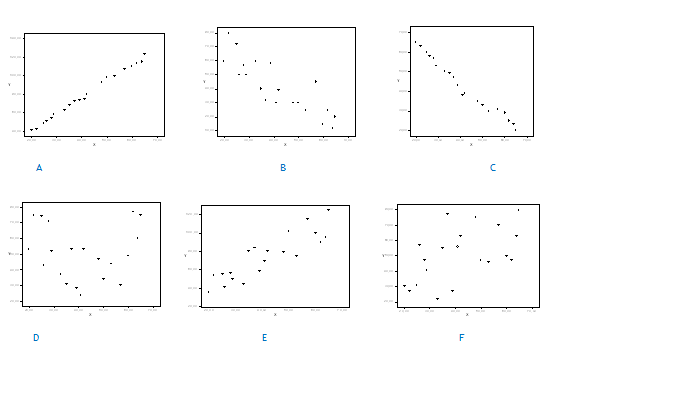
\includegraphics[width=1.10\textwidth]{images/correlaties.png}
	\captionof{figure}{Correlaties}
	\label{fig:correlaties}
%\end{figure}
\end{exercise}

\begin{exercise}
	\label{oef:Lineaire regressie, correlatie en determinatiecoëfficiënt met R}
	Lees het databestand ``Cats.csv'' in. 
		\begin{enumerate}
		\item Voer een lineaire regressieanalyse uit op de variabelen Lichaamsgewicht (Bwt) en Gewicht hart (Hwt).
		\item Maak een spreidingsdiagram van beide variabelen.
		\item Bereken en teken de regressielijn.
		\item Bereken de correlatie- en de determinatiecoëfficiënt.
		\item Geef een interpretatie van deze resultaten.
	\end{enumerate}
\end{exercise}

\begin{exercise}
	Gebruik dezelfde data als in vorige oefening.
		\begin{enumerate}
		\item Voer een lineaire regressieanalyse uit op de variabelen Lichaamsgewicht (Bwt) en Gewicht hart (Hwt) per geslacht.
		\item Maak een spreidingsdiagram van beide variabelen voor elk van de geslachten.
		\item Bereken en teken telkens de regressielijn.
		\item Bereken de correlatie- en de determinatiecoëfficiënt.
		\item Geef een interpretatie aan deze resultaten.
	\end{enumerate}
\end{exercise}

\begin{exercise}
	Lees het databestand ``Pizza.csv'' in.
		\begin{enumerate}
		\item Voer een volledige lineaire regressieanalyse uit op de variabelen Rating en CostPerSlice. Trek hieruit de juiste conclusies en ga deze ook grafisch na.
		\item Onderzoek een mogelijk verband tussen Rating en Neighbourhood. Welke methode kan je hiervoor gebruiken? Kan je de gegevens van Rating hiervoor in dezelfde vorm gebruiken?
		\item Geef een interpretatie aan deze resultaten.
		\item Stel de kruistabel grafisch voor met een staafdiagram.  Voorzie een legende.
	\end{enumerate}
\end{exercise}

\chapter{De \texorpdfstring{$\chi^{2}$}{Chi-kwadraat} toets}
\label{ch:chikwadraat}

\section{\texorpdfstring{$\chi^{2}$}{Chi-kwadraat} toets voor verdelingen}

Wanneer alle variabelen in het onderzoek nominaal zijn, is chi kwadraat de eenvoudigste (en populairste) techniek die men ter beschikking heeft voor het toetsten van hypothesen. De teststatistiek heet chi kwadraat, en is verdeeld volgens de chi kwadraat verdeling. De test kan gebruikt worden om na te gaan in welke mate de steekproef overeenstemt met een nulhypothese over de verdeling van de variabele. Men noemt dit een \textit{goodness of fit} \index{Test goodness of fit} test.

In het voorbeeld op de slides willen we nagaan, of de verdeling van onze steekproef bij $n = 400$ superhelden overeenstemt met de verdeling die je verwacht in de volledige populatie (de verzameling van alle mogelijke superhelden). 

Daartoe vergelijken we de aantallen in de steekproef met de aantallen die je zou verwachten als de steeproef exact representatief zou zijn naar de types van superhelden. Als deze verschillen relatief groot zijn dan komt de verdeling in de steekproef niet overeen met de verdeling in de populaties en zullen we moeten concluderen dat de steekproef niet representatief is. Om te oordelen of deze verschillen relatief groot zijn voeren we een $\chi^{2}$toets uit. 


\subsection{Voorbeeld superhelden}
We willen kijken of de steekproef voor onze superhelden representatief is. Als de steekproef exact representatief zou zijn zouden we verwachten dat in de steekproef 35\% van de superhelden een mutant zou zijn. Het verwachte aantal of de verwachte frequentie voor deze categorie is dus gelijk aan $0,35 \times 400 = 140$. De verwachte frequenties worden genoteerd met de letter $e$ (expected). Er geldt dus:

\[ e = n \times \pi \]

met $\pi$ de frequentie over de hele populatie. Als de verschillen $o - e$ ($o$ staat voor observed) reletief klein zijn kunnen ze toegerekend worden aan toevallige steekproeffouten. We gaan nu een toetsingsgrootheid bepalen waarmee getoetst kan worden of de steekproefverdeling overeenkomt met de gegeven verdeling in de populatie.

Beschouw $\chi^{2}$:

\[ \chi^{2} = \sum_{i=1}^{n} \frac{(o_{i} - e_{i})^{2}}{e_{i}} \]

We merken op:
\begin{itemize}
	\item indien de verschillen klein zijn $\Rightarrow$ verdeling komt voldoende overeen
	\item indien de verschillen groot $\Rightarrow$ verdeling niet representatief
\end{itemize}

We bepalen nu een kritieke grenswaarde $g$ die een $\chi^{2}$ verdeling heeft. Hierbij speel het aantal vrijheidsgraden een rol ($df$). Er geldt:

\[ df = k -1 \]

met $k$ het aantal categorie\"en. In ons voorbeeld hebben we $df = 5-1 = 4$. Om de kritieke grenswaarde te bepalen, kan je gebruik maken van een tabel voor de $\chi^2$-verdeling. Voor een gegeven significantieniveau $\alpha$ en vrijheidsgraad $df$ kan je in zo'n tabel de grenswaarde aflezen.

In ons voorbeeld is $\chi^{2} = 3,47$ met grenswaarde $g = 9,49$. Omdat de gevonden toetsingsgrootheid $\chi^2 = 3,47 < g = 9,49$, mogen we besluiten dat de steekproef representatief is.


\subsection{Toetsingsprocedure}
We volgen de stappen van een statistische toetsingsprocedure:

\begin{enumerate}
	\item \textbf{Bepalen hypotheses}
		Als nulhypothese formuleren we dat de verdeling over de opleidingen in de steekproef gelijk is aan de verdeling in de populatie. Als alternatieve hypothese formuleren we dat de verdelingen verschillend zijn.
		\begin{itemize}
			\item $H_{0}$: steekproef is representatief naar populatie
			\item $H_{1}$: steekproef is niet representatief naar populatie
		\end{itemize}
	\item \textbf{Bepalen $\alpha$ en $n$} : $\alpha = 0,05$ en $n = 400$.
	\item \textbf{Toetsingsgrootheid en waarde ervan in steekproef}:
	\[ \chi^{2} = \sum_{i=1}^{n} \frac{(o_{i} - e_{i})^{2}}{e_{i}} \]
	\item \textbf{Bereken en teken kritiek gebied}: de toets is altijd rechtszijdig. Is de toetsingsgrootheid kleiner dan kritieke grenswaarde verwerp $H_{0}$ niet, anders verwerp $H_{0}$ en aanvaard $H_{1}$. 
\end{enumerate}

\subsection{Voorbeeld 2}

Beschouw alle gezinnen met 5 kinderen in een bepaalde gemeenschap. Met betrekking tot samenstelling zijn er 6 mogelijkheden. 
\begin{enumerate}
	\item 5 jongens
	\item 4 jongens, 1 meisje
	\item 3 jongens, 2 meisjes
	\item 2 jongens, 3 meisjes
	\item 1 jongen, 4 meisjes
	\item 5 meisjes
\end{enumerate}

Het onderzoek bevat 1022 gezinnen met 5 kinderen en resultaten staan beschreven in de slides (kolom = aantal jongens). Zijn de waargenomen aantallen in de 6 klassen representatief voor een populatie waar de kans om een jongen te krijgen = kans om een meisje te krijgen = 0,5?

Indien de veronderstelling waar is wordt de kans $\pi_{i}$ om $i$ jongens te krijgen bepaald door een binominaalverdeling met parameters $n=5$ en $p=0,5$.

Dit kan je eenvoudig nagaan aan de hand van voorbeeld. De kans om 2 jongens te krijgen met 5 kinderen is gelijk aan :

\[ (0,5)^{2} \times (1-0,5)^{5-2} \times \binom{5}{2} \]
 
Algemeen geldt dus:

\[ \pi_{i} = \binom{5}{i}\times 0,5^{i} \times 0,5^{5-i} = \frac{5!}{i!(5-i)!}\times 0,5^{5} \]

Met deze $\pi_{i}$ kunnen we dus de verwachte waarde bepalen en de stappen volgen zoals hierboven beschreven. 

\begin{enumerate}
	\item \textbf{Bepalen hypotheses}
		
		\begin{itemize}
			\item $H_{0}$: steekproef is representatief naar populatie
			\item $H_{1}$: steekproef is niet representatief naar populatie
		\end{itemize}
	\item \textbf{Bepalen $\alpha$ en $n$} : $\alpha = 0,01$ en $n = 1022$.
	\item \textbf{Toetsingsgrootheid en waarde ervan in steekproef}:
	\[ \chi^{2} = \sum_{i=1}^{n} \frac{(o_{i} - e_{i})^{2}}{e_{i}} = 29,5766 \]
	\item \textbf{Bereken en teken kritiek gebied}:  kritieke grens is 15,0863. Onze toetsingsgrootheid ligt dus in het kritieke gebied dus verwerpen we $H_{0}$. 
\end{enumerate}

We vinden dus dat de steekproef niet representatief is naar een populatie waar geldt dat de kans op een jongen even groot is als de kans op een meisje. Het is interessant om te kijken naar de gestandaardiseerde residuen die aanduiden welke klassen de grootste bijdrage leveren aan de waarde van de grootheid. 

\[ r_{i} = \frac{O_{i} - n \pi_{i}}{\sqrt{n \pi_{i}(1-\pi_{i})}} \]

\begin{exercise}
	Hoe komen we hier aan de noemer? Waar komt dit mee overeen? Hoe bepaal je de variantie van een binomiale verdeling?
Antwoord: $n \times \pi (1-\pi)$
\end{exercise}



Er geldt algemeen dat waarden groter dan 2 of kleiner dan $-2$ extreem zijn. We kunnen dus besluiten dat het aantal gezinnen waarin alle kinderen hetzelfde geslacht hebben groter mag worden genoemd dan verwacht.

\subsection{Voorwaarden}
 Om de toets te mogen toepassen dient aan de volgende voorwaarden te zijn voldaan (Regel van Cochran)
\begin{enumerate}
	\item Voor alle categorie\"en moet gelden dat de verwachte waarde $e$ groter is dan 1.
	\item In ten hoogste 20 \% van de categori\"en mag de verwachte waarde $e$ kleiner dan 5 zijn.
\end{enumerate}


\section{\texorpdfstring{$\chi^{2}$}{Chi-kwadraat}-kruistabeltoets}
De Chi-kwadraattoets \index{$\chi^{2}$kwadraatkruistabeltoets} laat zich eenvoudig uitbreiden tot een onderzoeksontwerp
met twee variabelen, met respectievelijk $r$ en $k$ niveaus. Hier gaan we onderzoeken of er een verband is tussen 2 variabelen. De procedure kan opnieuw geformuleerd worden.

We gaan de procedure na aan de hand van een studie door \textcite{Doll1954} over de relatie tussen roken en longkanker. Doll en Hill schreven in 1951 alle Britse huisartsen aan met het verzoek om gegevens over hun leeftijd en rookgedrag. Vervolgens hielden ze jarenlang de overlijdensberichten en de doodsoorzaak bij en herhaalden hun periodiek. De eerste uitkomsten, na circa vier jaar, zijn in tabel~\ref{tab:dollhill} samengevat. Uit de tabel kan makkelijk geconcludeerd worden dat er geen relatie is tussen roken en longkanker. In (ruim) vier jaar is slechts $(84 / 24354) * 100 = 0,35\% $ van de Britse artsen aan longkanker overleden en dat met slechts $(83 / 21261) * 100 = 0,39\%$ van de rokers onder hen. Dit is weinig, maar het is wel veel meer dan hetzelfde cijfer voor de niet-rokers $(1 / 3093) * 100 = 0,032\%$.


\begin{table}
  \begin{center}
    \begin{tabular}{@{}lllll@{}}
      \toprule
                       & \textbf{Longkanker} & \textbf{Niet} & \textbf{Wel} & \textbf{Totaal} \\
        \midrule
        \textbf{Roker} & \textbf{Wel}        & 21178         & 83           & 21261           \\
                       & \textbf{Niet}       & 3092          & 1            & 3093            \\
                       & \textbf{Totaal}     & 24270         & 84           & 24354           \\
        \bottomrule
    \end{tabular}
  \end{center}
  \caption{Resultaten van het onderzoek van~\textcite{Doll1954}}
  \label{tab:dollhill}
\end{table}

We zien in de tabel dat er wel een erg groot verschil is tussen de geobserveerde aantallen rokers die overlijden aan longkanker en de verwachte waarden in deze cel. Hetzelfde geldt voor het geringe aantal huisartsen dat niet rookt, maar wel aan longkanker overleden is. Deze observatie maakt ons wel wantrouwig of de eerdere tentatieve conclusie wel juist is. We kunnen afrekenen met deze onzekerheid door de toetsingsgrootheid $\chi^{2}$ uit te rekenen. Dat doen we op de vertrouwde manier:


\begin{enumerate}
	\item \textbf{Bepalen hypotheses}	
		\begin{itemize}
			\item $H_{0}$: in de populatie is er geen samenhang tussen onafhankelijke en afhankelijke variabele
			\item $H_{1}$: er bestaat wel een samenhang tussen de variabelen in de populatie
		\end{itemize}
	\item \textbf{Bepalen $\alpha$ en $n$} : $\alpha = 0,05$ en $n = 24354$.
	\item \textbf{Toetsingsgrootheid en waarde ervan in steekproef}:
	\[ \chi^{2} = \sum_{i=1}^{n} \frac{(o_{i} - e_{i})^{2}}{E_{i}} = 10,35 \]
	\item \textbf{Bereken en teken kritiek gebied}:  kritieke grens is 3,8415 en aantal vrijheidsgraden $df = (r-1)(k-1)$ Onze toetsingsgrootheid ligt dus in het kritieke gebied dus verwerpen we $H_{0}$. 
\end{enumerate}

We moeten derhalve $H_{0}$, dat er geen relatie is tussen beide variabelen, verwerpen ten gunste van $H_{1}$ dat er wel een relatie is tussen beide variabelen: rokers sterven vaker aan longkanker dan niet-rokers.

Maar, is dit nu een bewijs dat zoals zo vaak verondersteld wordt dat roken longkanker veroorzaakt? Nee, dat is het absoluut niet. Een paar alternatieve verklaringen: niet alle rokers krijgen longkanker, de rokers zijn ouder dan de niet-rokers, de rokers wonen veelal in de grote steden met
meer vervuilde lucht dan de niet-rokers die veelal op het platte land wonen, ook zou er nog een speciale genetische dispositie kunnen zijn, die zowel van invloed is op de verslaving aan tabak, als op de kans om longkanker te krijgen. Voor een causale interpretatie van de gegevens (let wel, het betreft hier immers geen experiment), moeten we op zijn minst de beschikking hebben over een theorie die de relatie tussen roken en longkanker expliciteert.

\section{Oefeningen}
\label{sec:chi-kwadraat-oefeningen}

\begin{exercise}
  \label{ex:chisq-survey}
  Voor deze oefening maken we gebruik van de dataset \texttt{survey} die is meegeleverd met R. De dataset is samengesteld uit een bevraging onder studenten. Om deze te laden, doe het volgende:
  
  \begin{lstlisting}
  library(MASS)
  View(survey)  # Toont de "survey" dataset
  ?survey       # Help-pagina voor deze dataset met uitleg over de inhoud
  \end{lstlisting}
  
  Als je een foutboodschap krijgt bij het laden van de bibliotheek (eerste regel), betekent dit dat de package \texttt{MASS} nog niet geïnstalleerd is. Dit kan je alsnog doen via Tools > Install Packages en het invullen van de package-naam in het tekstveld.
  
  We willen de relatie onderzoeken tussen enkele discrete (nominale of ordinale) variabelen in deze dataset. Voor elke hieronder opgesomde paren, volg deze stappen:
  
  \begin{enumerate}[label=(\alph*)]
    \item Denk eerst eens na welke uitkomt je precies verwacht voor de opgegeven combinatie van variabelen.
    \item Stel een frequentietabel op voor de twee variabelen. De (vermoedelijk) onafhankelijke variabele komt eerst.
    \item Plot een grafiek van de data, bv.~geclusterde staafgrafiek, gestapelde staafgrafiek van relatieve frequenties, of een ``mozaïekgrafiek'' (eenvoudig met \texttt{plot(table(data\$col1, data\$col2))}).
    \item Als je de grafiek bekijkt, verwacht je dan een eerder hoge of eerder lage waarde voor de $\chi^2$-statistiek? Waarom?
    \item Bereken de $\chi^2$-statistiek en de kritieke grenswaarde $g$ (voor significantieniveau $\alpha = 0.05$)
    \item Bereken de $p$-waarde
    \item Moeten we de nulhypothese aanvaarden of verwerpen? Wat betekent dat concreet voor de relatie tussen de twee variabelen?
  \end{enumerate}

  Hieronder zijn de te onderzoeken variabelen opgesomd. De vermoedelijke onafhankelijke variabele komt telkens eerst.
  
  \begin{enumerate}
    \item \texttt{Exer} (sporten) en \texttt{Smoke} (rookgedrag)
    \item \texttt{W.Hnd} (de hand waarmee je schrijft) en \texttt{Fold} (de hand die bovenaan komt als je de armen kruist)
    \item \texttt{Sex} (gender) en \texttt{Smoke}
    \item \texttt{Sex} en \texttt{W.Hnd}
  \end{enumerate}
\end{exercise}

\begin{exercise}
  \label{ex:chisq-aids2}
  Laad de dataset \texttt{Aids2} uit package \texttt{MASS} (zie Oefening~\ref{ex:chisq-survey}) die informatie bevat over 2843 patiënten die vóór 1991 in Australië met AIDS besmet werden. Deze dataset werd in detail besproken door~\textcite{Ripley2007}. Onderzoek of er een relatie is tussen de variabele geslacht (\texttt{Sex}) en de manier van besmetting (\texttt{T.categ}).
  
  \begin{enumerate}
    \item Ga op de gebruikelijke manier te werk: visualiseren van de data, $\chi^2$, $g$ en $p$-waarde berekenen ($\alpha = 0,05$), en tenslotte een conclusie formuleren.
    \item Bepaal de gestandaardiseerde residuën om te bepalen welke categorieën extreme waarden bevatten.
  \end{enumerate}
  
\end{exercise}

\begin{exercise}
  \label{ex:chisq-digimeter}
  
  Elk jaar voert Imec (voorheen iMinds) een studie uit over het gebruik van digitale technologieën in Vlaanderen, de Digimeter~\autocite{Vanhaelewyn2016}. In deze oefening zullen we nagaan of de steekproef van de Digimeter 2016 ($n = 2164$) representatief is voor de bevolking wat betreft de leeftijdscategorieën van de deelnemers.
  
  In Tabel~\ref{tab:digimeter2016} worden de relatieve frequencies van de deelnemers weergegeven. De absolute frequenties voor de verschillende leeftijdscategorieën van de Vlaamse bevolking worden samengevat in Tabel~\ref{tab:leeftijd-vlaanderen}. Deze gegevens zijn ook te vinden in bijgevoegd CSV-bestand \texttt{oefeningen/data/bestat-vl-ages.csv}.
  
  \begin{enumerate}
    \item De tabel met leeftijdsgegevens van de Vlaamse bevolking als geheel heeft meer categorieën dan deze gebruikt in de Digimeter. Maak een samenvatting zodat je dezelfde categorieën overhoudt dan deze van de Digimeter. Tip: dit gaat misschien makkelijker in een rekenblad dan in R.
    \item Om de goodness-of-fit test te kunnen toepassen hebben we de absolute frequenties nodig van de geobserveerde waarden in de steekproef. Bereken deze.
    \item Bereken ook de verwachte percentages ($\pi_{i}$) voor de populatie als geheel.
    \item Voer de goodness-of-fit test uit over de verdeling van leeftijdscategorieën in de steekproef van de Digimeter. Is de steekproef in dit opzicht inderdaad representatief voor de Vlaamse bevolking?
  \end{enumerate}
\end{exercise}

\begin{table}
  \caption{Frequenties van de leeftijd van deelnemers aan de iMec Digimeter 2016 en de Vlaamse bevolking.}
  \label{tab:frequenties-leeftijden}
  \centering
  \begin{tabular}{cc}
    \textbf{Leeftijdsgroep} & \textbf{Percentage} \\ \midrule
    15-19 & 6,6\% \\
    20-29 & 14,2\% \\
    30-39 & 15,0\% \\
    40-49 & 16,3\% \\
    50-59 & 17,3\% \\
    60-64 & 7,3\% \\
    64+   & 23,2\% \\
  \end{tabular}
  \subcaption{Percentage van deelnemers aan de Digimeter 2016 van iMec ($n = 2164$), opgedeeld per leeftijdscategorie. \autocite{Vanhaelewyn2016}}
  \label{tab:digimeter2016}
  
  \centering
  \begin{tabular}{cc}
    \textbf{Leeftijdsgroep} & \textbf{Aantal} \\ \midrule
              –5            &     352017      \\
              5-9           &     330320      \\
             10-14          &     341303      \\
             15-19          &     366648      \\
             20-24          &     375469      \\
             25-29          &     387131      \\
             30-34          &     401285      \\
             35-39          &     409587      \\
             40-44          &     458485      \\
             45-49          &     493720      \\
             50-54          &     463668      \\
             55-59          &     413315      \\
             60-64          &     379301      \\
             65-69          &     299152      \\
             70-74          &     279789      \\
             75-79          &     249260      \\
             80-84          &     182352      \\
             85-89          &     104449      \\
             90-94          &      29888      \\
             95-99          &      7678       \\
             100+           &       923
  \end{tabular}
  \subcaption{Absolute frequentie van de Vlaamse bevolking per leeftijdscategorie. Bron: BelStat (\url{https://bestat.economie.fgov.be/bestat/}, C01.1: Bevolking volgens verblijfplaats (provincie), geslacht, positie in het huishouden (C), burgerlijke staat en leeftijd (B)).}
  \label{tab:leeftijd-vlaanderen}
  

\end{table}

\section{Antwoorden op geselecteerde oefeningen}
\label{sec:chi-kwadraat-oplossingen}

\paragraph{Oefening~\ref{ex:chisq-survey}}

\begin{enumerate}
  \item \texttt{Exer}/\texttt{Smoke}: $\chi^2 = 5.49$, $g = 12.5916$, $p = 0.35$
  \item \texttt{W.Hnd}/\texttt{Fold}: $\chi^2 = 1.581399$, $g = 5.9915$, $p = 0.454$
  \item \texttt{Sex}/\texttt{Smoke}: $\chi^2 = 3.554$, $g = 7.8147$, $p = 0.314$
  \item \texttt{Sex}/\texttt{W.Hnd}: $\chi^2 = 0.236$, $g = 3.8415$, $p = 0.627$
\end{enumerate}

\paragraph{Oefening~\ref{ex:chisq-aids2}} $\chi^2 = 1083.372914$, $g = 14.067140$, $p \approx 1.157 \times 10^{-229}$

\paragraph{Oefening~\ref{ex:chisq-digimeter}} $\chi^2 = 6.6997$, $g = 12.5916$, $p = 0.35$

\chapter{Tijdreeksen}

\section{Tijdreeksen \& voorspellingen}

\begin{definition}[Tijdsreeks]
	Een tijdreeks is een opeenvolging van observaties van een willekeurige variabele in functie van de tijd.
\end{definition}

Een tijdreeks is dus eens stochastisch proces. Denk hierbij maar aan:
\begin{itemize}
	\item maandelijkse vraag naar melk
	\item jaarlijkse instroom van studenten bij de Hogeschool
	\item dagelijks debiet van een rivier
	\item verkoop van een bepaalde order bij een bedrijf
\end{itemize}

Het voorspellen van tijdreeksen is een belangrijk onderdeel van onderzoek omdat ze vaak de basis vormen voor beslissingsmodellen. Voorbeelden hiervan zijn :

\begin{itemize}
	\item algemene ontwikkeling van toekomstplannen (investeringen, capaciteit \dots)
	\item plannen van budgettering om tekortkomingen te vermijden (operationeel budget, marketing budget \dots)
	\item competitieve leveringstijden van een bedrijf
	\item ondersteuning van financi\"ele objectieven
	\item onzekerheid vermijden
	\item de mogelijkheid om ontwikkelingen in de verkeersveiligheid
kwantitatief te modelleren
\end{itemize}

Tijdreeksen modelleren is een statistisch probleem: we gaan ervan uit dat de observaties vari\"eren volgens een bepaalde kansdichtheidsfunctie in functie van de tijd. Vaak gaan we ervan uit dat de observaties in een tijdsreeks gecorreleerd zijn en dus niet uit een random sample komen. 

Er zijn verschillende types modellen in gebruik voor het analyseren van tijdreeksen. Deze modellen hebben met elkaar gemeen dat ze in principe niet alleen de ontwikkeling in een geobserveerde tijdreeks kunnen beschrijven, maar dat we ze ook kunnen gebruiken om
\begin{inparaenum}[(i)]
	\item verklaringen te vinden voor die ontwikkeling en
	\item om de toekomstige waarden van de tijdreeks te voorspellen
\end{inparaenum}
Hun geschiktheid voor het verwezenlijken van deze doelstellingen loopt echter sterk uiteen. In dit hoofdstuk beperken we ons tot het gebruik van tijdreeksen met een geschiedenis om tijdsafhankelijke modellen te bepalen. Een voorbeeld van een tijdsreeks is bijvoorbeeld de leeftijd van de opeenvolgende koningen van Engeland startend van Willem De Veroveraar \autocite{Hipel194}.
\begin{lstlisting}
kings <- scan(file = 'Documents/education/onderzoekstechnieken-cursus/cursus/data/tijdsreeksen/kings.data', skip = 3)
kingstimeseries <- ts(kings)
plot.ts(kingstimeseries, ylab='leeftijd', xlab="tijd")
grid(lty=2,lwd=1,col='black')
\end{lstlisting}

\begin{figure}[htbp]
	\centering
	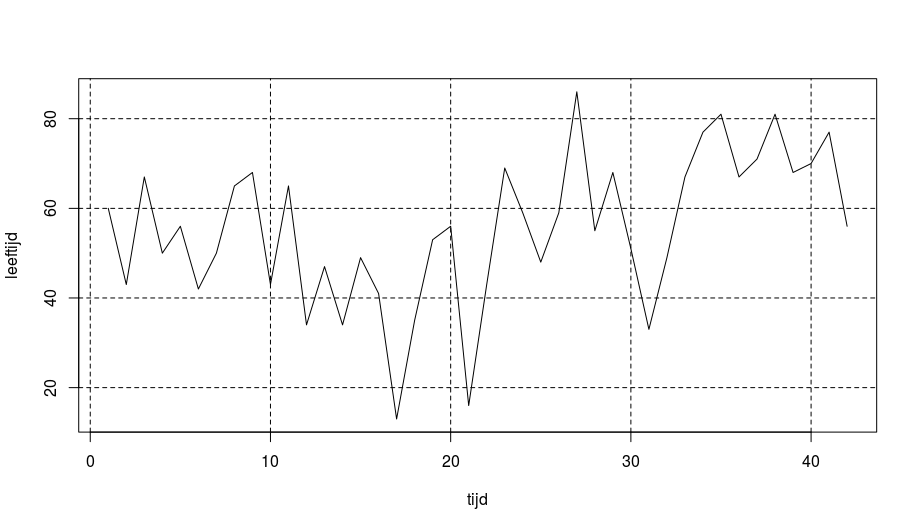
\includegraphics[width=\textwidth]{images/tijdsreeksen/tijdsreekskings.png}
	\caption{De tijdsreeks die de leeftijden van de koningen voorstelt.}
	\label{fig:tijdreeks11}
\end{figure}


\section{Tijdreeksmodellen}
\subsection{Wiskundig model}
Ons doel is het opstellen van een model dat een verklaring vindt voor de geobserveerde data en dat toelaat om observaties in de toekomst zo goed mogelijk te voorspellen. Het simpelste model dat je kan bedenken is een model waarbij een constante $b$ gebruikt wordt met variaties rond $b$ bepaald door een willekeurige variabele $\epsilon_{t}$ zoals in vergelijking \ref{eq:constante}. 

\begin{equation}
	X_{t} = b + \epsilon_{t}
\label{eq:constante}
\end{equation}

\begin{description}
	\item [$X_{t}$] stelt een \textit{variabele} voor dat de onbekende is op tijdstip $t$.
	\item [$x_{t}$] stelt een \textit{observatie} voor op tijdstip $t$ (en is dus gekend). 
	\item [$\epsilon_{t}$] noemt met de \textit{storing} (engels \textsl{noise}) en wordt geacht een gemiddelde van $0$ te hebben met variantie $\sigma^{2}$ en normaal verdeeld. 
\end{description}




We kunnen ook ervan uit gaan dat er een lineair verband is:

\begin{equation}
	X_{t} = b_{0} + b_{1} \times t + \epsilon_{t}
\label{eq:lineair8}
\end{equation}

De vergelijking in \ref{eq:constante} en \ref{eq:lineair8} zijn speciale gevallen van het polynomiaal geval:

\begin{equation}
	X_{t} = b_{0} + b_{1} t + b_{2} t^{2} + \dots + b_{n} t^{n} + \epsilon_{t} 
\label{eq:polynomiaal}
\end{equation}

\begin{exercise}
	Wat zou volgende tijdreeks kunnen voorstellen?
	\begin{equation}
		X_{t} = b_{0} + b_{1} \sin(\frac{2\pi t}{4}) + b_{1} \cos(\frac{2\pi t}{4}) + \epsilon_{t}
	\label{eq:seasonal}
\end{equation}
\end{exercise}

\begin{solution}
Antwoord: dit is een cyclische tijdreeks met periode $= 4$. Dit zou bijvoorbeeld kunnen gebruikt worden bij een tijdreeks voor seizoenen. 

\begin{lstlisting}
f <- function(a, b,t){
	return(a + b * sin((2 * pi*4)/4) + b * cos((2 * pi*4)/4) + rnorm(1))
}
t <- seq(from = 1, to = 100, by = 1)
X <- lapply(t,f,a=5,b=5)
plot(x = t, y=X, type = 'l')
\end{lstlisting}
	
\end{solution}



\subsubsection{Algemeen}

In elk model beschouwd is de tijdreeks een functie van tijd en parameters van het model. We kunnen algemeen stellen dat:

\begin{equation}
	X_{t} = f(b_{0}, b_{1}, b_{2}, \dots , b_{t}, t) + \epsilon_{t}
\label{eq:general}
\end{equation}

We aanvaarden vervolgens nog volgende stellingen:
\begin{itemize}
	\item Het model gaat uit van twee componenten van variabiliteit: het gemiddelde van de voorspellingen verandert met de tijd en de variaties tot dit gemiddelde vari\"eren willekeurig.
	\item De residuen van het model ($X_{t} - x_{t}$) zijn homoscedastisch : dat wil zeggen in de tijd een constante variantie hebben.
\end{itemize}

Eenmaal het model gekozen, rest enkel nog het  probleem van het schatten van de parameters voor vergelijking \ref{eq:general}. Dit is wat in de volgende stukken besproken zal worden.

\section{Schatten van de parameters}
Eenmaal een model geselecteerd wordt, is het aan de onderzoeker om de parameters te gaan schatten, i.e. parameters die ervoor zorgen dat het model de geobserveerde waarden zo goed mogelijk benaderen. Meestal gaan we ervan uit dat alle waarden gelijkwaardig zijn, maar dat is niet zo bij tijdreeksen. Aangezien onze onafhankelijke parameter de tijd is moeten we methoden bekomen die ervoor zorgen dat recentere data belangrijker zijn dat oude data of omgekeerd. 

In wat volgt beschrijven we de tijdreeksen met geschatte waarden voor de parameters. We zetten hievoor een hoedje op de parameters:

\[ \widehat{b}_{1}, \widehat{b}_{2} \dots \widehat{b}_{n} \] 

\subsection{Voorbeeld - moving average}

\begin{table}[t]
\centering
    \begin{tabular}{|l|l|l|l|l|l|l|l|l|l|}
    \hline
    4 & 16 & 12 & 25 & 13 & 12 & 4 & 8  & 9 & 14 \\ \hline
    3 & 14 & 14 & 20 & 7  & 9  & 6 & 11 & 3 & 11 \\ \hline
    8 & 7  & 2  & 8  & 8  & 10 & 7 & 16 & 9 & 4  \\ \hline
    \end{tabular}
    \caption{Voorbeeld data van vraag voor product, zie figuur \ref{fig:tijdreeks11}}
    \label{tab:data}
\end{table}

Stel dat de statisticus de data in tabel \ref{tab:data} tot het twintigste datapunt beschikbaar heeft (bekende data). De onderzoeker kent de datapunten vanaf het twintigste datapunt niet en moet deze gaan voorspellen. Een eerste model dat gebruikt zou kunnen worden is het constante model zoals in \ref{eq:constante}. 

Met dit model, zijn de waarden random waarden uit een populatie met gemiddelde $b$. De beste schatter voor $b$ is het gemiddelde van deze twintig data punten. 

\begin{lstlisting}
	data <- c(4 , 16 , 12 , 25 , 13 , 12 , 4 , 8  , 9 , 14, 
	+           3 , 14 , 14 , 20 , 7  , 9  , 6 , 11 , 3 , 11, 
	+           8 , 7  , 2  , 8  , 8  , 10 , 7 , 16 , 9 , 4 )
	mean(data[1:20])
\end{lstlisting}

\[ \widehat{b} = \frac{1}{20} \sum_{1}^{20} x_{t}= 10.75 \] 

Dit is de beste schatter vertrekkende van de 20 datapunten. We merken wel op dat $x_{1} =  4$ evenveel \textit{waarde} heeft als $x_{20} = 11$, of ander verwoord: de co\"effici\"ent van  $x_{1}$ is dezelfde als die van $x_{20}$, namelijk $\frac{1}{20}$.

Indien we dit als schatter zouden gebruiken dan zien we dat dit in figuur \ref{fig:tijdreeks21} geen goed idee is.

\begin{lstlisting}
AV20 <- matrix(10.75,30,1)
plot.ts(data, col="blue", type='b', xlab='tijd', ylab='Data')
lines(AV20,col='red', type='l')
legend(x= 'topright',legend = c("Data","Average 10.75"), lty = c(1,1), lwd = c(2.5,2.5), col=c('blue','red'))
\end{lstlisting}

\begin{figure}[htbp]
	\centering
		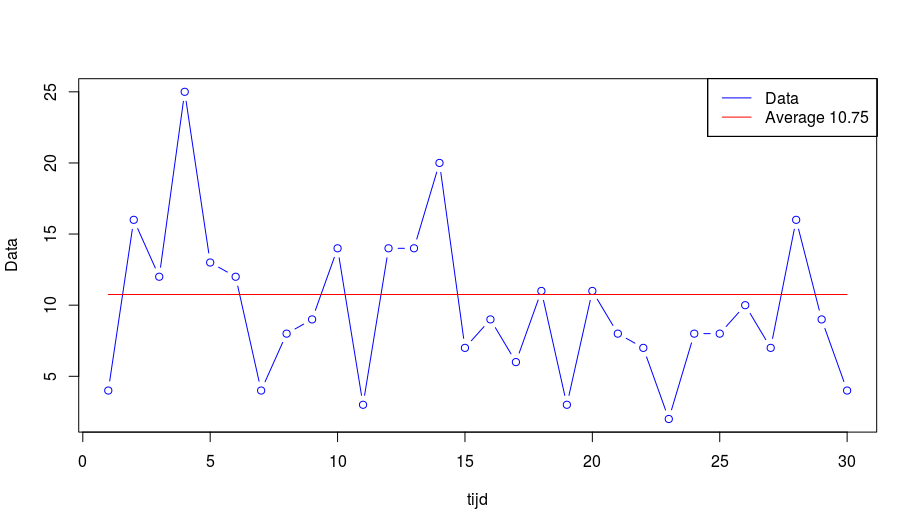
\includegraphics[width=1.00\textwidth]{images/tijdsreeksen/tijdsreeks20.png}
	\caption{Tijdreeks met constant gemiddelde $10.75$}
	\label{fig:tijdreeks21}
\end{figure}


Indien we veronderstellen dat de data verandert met de tijd is het beter om oude data minder waarde te geven en de recente data meer waarde. Een mogelijkheid is om enkel recente data te gebruiken, bijvoorbeeld de 10 en 5 laatste datapunten (zie figuur \ref{fig:tijdreeks31}).

\[ \widehat{b} = \frac{1}{10} \sum_{10}^{20} x_{t} = 10.18 \] en
\[ \widehat{b} = \frac{1}{5} \sum_{15}^{20} x_{t} = 7.83 \]

\begin{lstlisting}
sma10 <- SMA(x =data,n=10)
sma5 <- SMA(x=data,n=5)
plot.ts(x = data, col = 'blue',type = 'l')
lines(sma10, col='red', type = 'b')
lines(sma5, col='purple', type = 'b')
\end{lstlisting}

\begin{figure}
	\centering
		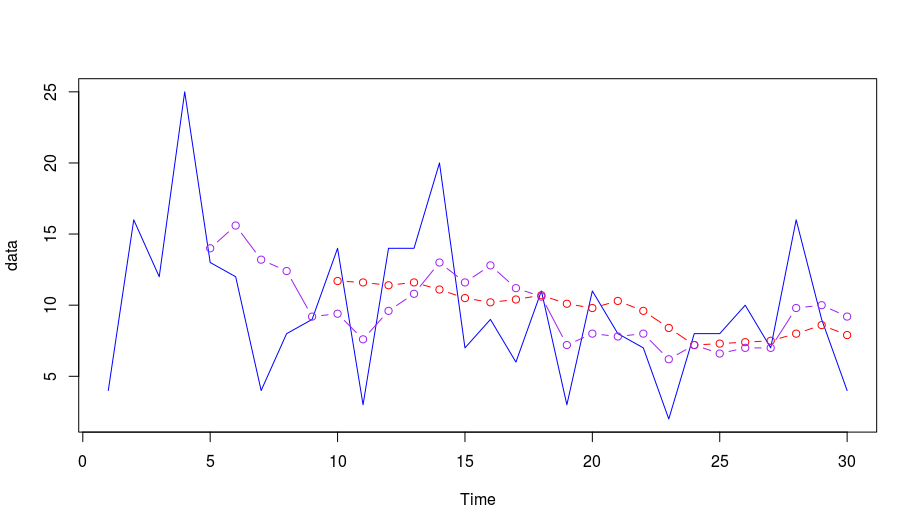
\includegraphics[width=1.00\textwidth]{images/tijdsreeksen/tijdsreekssma.png}
		\caption{Tijdreeks met moving average $m = 10$ en $m=5$}. 
	\label{fig:tijdreeks31}
\end{figure}




Dit worden \textit{moving averages} genoemd \index{moving average}. 

Welke schatter is nu de beste? We kunnen dit nu nog niet zeggen. 
\begin{itemize}
	\item De schatter die alle datapunten gebruikt is de beste indien de tijdreeks het model volledig volgt.
	\item De schatter met de recentere datapunten is de beste indien de tijdreeks verandert met de tijd.
\end{itemize}

\begin{definition}
	Algemeen is het moving average het gemiddelde van de $m$ laatste observaties.
	\begin{equation}
		\widehat{b} = \sum_{i=k}^{t} \frac{x_{i}}{m}
	\label{eq:movingAverage}
	\end{equation}
	met $k = t-m+1$. $m$ is de time range en is de parameter van de methode.
\end{definition}

\pagebreak
\subsection{Meten van de nauwkeurigheid van voorspellingen}

\begin{table}[h]
	\begin{tabular}{|lllllllllll|}
		\hline
		~         & 11   & 12   & 13   & 14   & 15   & 16   & 17   & 18   & 19   & 20   \\
		Data      & 3    & 14   & 14   & 20   & 7    & 9    & 6    & 11   & 3    & 11   \\
		Schatting & 11.7 & 11.6 & 11.4 & 11.6 & 11.1 & 10.5 & 10.2 & 10.4 & 10.7 & 10.1 \\
		Error     & -8.7 & 2.4  & 2.6  & 8.4  & -4.1 & -1.5 & -4.2 & 0.6  & -7.7 & 0.9  \\ \hline
	\end{tabular}
	\caption{Voorspellingsfout voor een moving average $m = 10$}
	\label{tab:error}
\end{table}


Een methode om de voorspelling te meten is het gemiddelde van de deviaties ($MAD$): gemiddelde absolute verschil tussen het voorspelde en de werkelijke waarden van de tijdsreeks.

\begin{definition}[$MAD$]
\begin{equation}
	MAD = \frac{1}{n} \sum_{1}^{n} \left| e_{i} \right|  
\label{eq:MAD}
\end{equation}
\end{definition}

Je kan dit ook percenteren om zo tot de gemiddelde absolute procentuele afwijking ($MAPE$) te komen.

\begin{definition}[$MAPE$]
\begin{equation}
	MAPE = \frac{1}{n} \sum_{1}^{n} \left| \frac{e_{i}}{X_i} \right|  
\label{eq:MAD2}
\end{equation}
\end{definition}


Je kan ook de variantie ervan bepalen:

\begin{definition}[$VAR$]
\begin{equation}
	s^{2}_{e} = \frac{1}{m} \sum_{1}^{n} (e_{i} - \overline{e})^{2}
\label{eq:varError}
\end{equation}
\end{definition}

Als laatste interessante parameter kan gekeken worden naar de wortel uit de gemiddelde kwadratische afwijking ($RMSE$), als de wortel uit het gemiddelde kwadratische verschil tussen de voorspelde en de werkelijke waarden van de tijdsreeks.

\begin{definition}[$RMSE$]
\begin{equation}
	RMSE_{e} = \sqrt{\frac{1}{m} \sum_{1}^{n} (e_{i})^{2}}
\label{eq:varError2}
\end{equation}
\end{definition}

\pagebreak
\section{Exponenti\"ele smoothing}
Bij een moving average krijgen alle voorgaande observaties een gelijk gewicht. Bij exponentieel smoothing worden kleinere gewichten toegekend aan oudere observaties. M.a.w.: recente observaties krijgen relatief meer gewicht dan oudere observaties.

In het geval van moving average zijn de gewichten hetzelfde, namelijk $\frac{1}{m}$.

\subsection{Enkelvoudige exponenti\"ele smoothing}
Exponenti\"ele effening (of smoothing) is een gewogen gemiddlede dat positieve gewichten toekent aan de huidige waarden en waarden uit het verleden van de tijdsreeks. Een enkel gewicht, $0\leq \alpha \leq1$ of de exponentie\"ele effeningsconstante wordt hiervoor gekozen. 
Voor een tijdseenheid $T$ wordt het enkelvoudige exponenti\"ele smoothing gevonden door vergelijking \ref{eq:singleExpSmooting}.

\begin{definition}[Exponenti\"ele smoothing]
\begin{equation}
	X_{T} = \alpha x_{t} + (1-\alpha)X_{t-1}, 0 \leq \alpha \leq 1, t \geq 3
\label{eq:singleExpSmooting}
\end{equation}
\end{definition}

$\alpha$ wordt de smoothing constante genoemd. Met andere woorden,$X_{T}$ is een gewogen gemiddelde van de huidige waarneming $x_t$ en de vorige exponenti\"ele smooting $X_{t-1}$.


\subsubsection{Inti\"ele setting}
Het bepalen van $X_{2}$ is een belangrijke parameter. Men kan kiezen om:
\begin{enumerate}
	\item $X_{2} = x_{1}$ te stellen
	\item $X_{2}$ gelijk te stellen aan een bepaald objectief
	\item Een gemiddelde te nemen van de eerste $x$ observaties
	\item \dots
\end{enumerate}

\begin{exercise}
	Waarom wordt dit een exponenti\"ele methode genoemd?
\end{exercise}
Antwoord: als we zouden substitueren vinden we bv. voor $X_{t-1}$:

\[ X_{t} = \alpha x_{t} + (1-\alpha)\left[\alpha x_{t-1} + (1-\alpha)X_{t-2}\right] \] 
\[ X_{t} = \alpha x_{t-1} + \alpha (1-\alpha)x_{t-1} + (1-\alpha)^{2} X_{t-2} \]
of dus algemeen gesteld :
\[ X_{t} = \alpha \sum_{i=0}^{t-2}(1-\alpha)^{i-1}x_{t-i} + (1-\alpha)^{t-2} X_{2}, t \geq 2 \]

Zo merk je dat oudere componenten een exponentieel kleiner gewicht verkrijgen. 

\subsubsection{Waarde voor $\alpha$}
De snelheid waarmee de oude observaties ''vergeten`` worden hang af van $\alpha$. Met een $\alpha$ dicht bij 1 vergeet je snel, terwijl een $\alpha$ dicht bij nul ervoor zorgt dat vergeten minder snel gaat (zoals aangetoond in tabel \ref{tab:alpha}). Vaak wordt een waarde gebruikt tussen $0.10$ en $0.30$.

\begin{table}
\centering
    \begin{tabular}{l|llll}
    $\alpha$ & $(1-\alpha)$ & $(1-\alpha)^{2}$ & $(1-\alpha)^{3}$ & $(1-\alpha)^{4}$ \\ \hline
    0.9   & 0.1       & 0.01             & 0.001                      & 0.0001           \\
    0.5   & 0.5       & 0.25             & 0.125                      & 0.062            \\
    0.1   & 0.9       & 0.81             & 0.729                      & 0.6561           \\
    \end{tabular}
		\caption{Waarden voor $\alpha$ en $(1-\alpha)^{n}$}
		\label{tab:alpha}
\end{table}


Bijvoorbeeld, het bestand \texttt{precip.data} bevat totale jaarlijkse neerslag in inches voor Londen, vanaf 1813-1912. Laten we dit eens analyseren met R.
\begin{lstlisting}
rain <- scan("Documents/education/onderzoekstechnieken-cursus/cursus/data/tijdsreeksen/precip.data",skip=1)
rainseries <- ts(rain,start=c(1813))
plot.ts(rainseries)
plot(rainseriesforecasts)
\end{lstlisting} 

%TODO figuur maken voor verschillende alpha's

\subsubsection{Voorspelling met exponenti\"ele effening}
Stel dat het doel is om de volgende waarde $X_{t+1}$ te voorspellen, dan wordt dit gelijk gesteld aan de smoothing waarde op tijdstip $t$.

\begin{equation}
	X_{t+1} = EMA_t = X_t
	\label{eq:EMA}
\end{equation}
Met $X_t$ de laatst voorspelde waarde. 

 We kunnen dit eenvoudig uitvoeren in R. Je krijgt hierbij een prediction interval: 
 Een prediction interval geeft een interval waarin we verwachten dat de voorspelde waarde met een bepaalde waarschijnlijkheid zal liggen. Standaard krijg je een 80\% en een 95\% interval. 
\begin{lstlisting} 
library('forecast')
rainseriesforecasts2 <- forecast.HoltWinters(rainseriesforecasts, h=8)
plot.forecast(rainseriesforecasts2)
\end{lstlisting} 

We zouden correlaties mogen zien tussen de voorspellingsfouten voor opeenvolgende voorspellingen. Met andere woorden, als er sprake is van een correlatie tussen prognosefouten voor opeenvolgende voorspellingen, is het eerder waarschijnlijk dat de simpele exponentiële effening kan worden verbeterd door een andere voorspellingstechniek te gebruiken.

Om te achterhalen of dit het geval is, kunnen we een correlogram verkrijgen van de in-sample voorspellingsfouten voor.

We weten nog uit hoofdstuk \ref{ch:analyse2var} dat de covariantie of correlate de lineaire relatie beschrijft tussen twee variabelen. . De autocovariantie en autocorrelatie meten de lineaire relatie tussen \textit{lagged} waarden voor een tijdsreeks. Met lagged bedoelen we een aantal stappen terug in de tijd.

\begin{definition}[Autocovariantie]
	We defini\"eren de autocovariantie bij lag $k$ door $c_k$.
	\[ c_k = \sum_{t=k+1}^{T} (y_t - \overline{y})(y_{t-k} - \overline{y}) \]
\end{definition}

\begin{definition}[Autocorrelatie]
	We defini\"eren de autocorrelatie bij lag $k$ door $r_k$.
	\[ r_k = \frac{c_k}{c_0} \]
\end{definition}

 We kunnen een correlogram die de autocorrelaties tekent, berekenen van de voorspellingsfouten met behulp van de functie 'acf ()' in R. Om de maximale lag te bepalen die we willen bekijken, gebruiken we de parameter 'lag.max' in acf ().

Bijvoorbeeld, om een ​​correlogram te berekenen van de in-steekprognosefouten voor de London-regenvalgegevens voor lags 1-20, typen we:

\begin{lstlisting}
	acf(rainseriesforecasts2$residuals, lag.max=20, na.action = na.pass)
\end{lstlisting}

Om te testen of er significant bewijs is voor significante correlaties bij lags 1-20, kunnen we een Ljung-Box test uitvoeren. Dit kan in R worden gedaan met de functie "Box.test ()". De maximale vertraging die we willen bekijken, wordt gespecificeerd met behulp van de parameter "Lag" in de Box.test () functie.

De test volledig uitleggen is buiten het bereik van deze cursus, maar de test gaat uit van volgende $H_0$ en $H_1$. De teststatistieken kunnen dan gewoon ge\"intepreteerd worden zoals alle andere hypothesetesten die beschreven geweest zijn in vorige hoofdstukken. 

\begin{itemize}
	\item $H_0$ De gegevens zijn onafhankelijk verdeeld (d.w.z. de correlaties in de populatie waaruit de sample wordt genomen, zijn 0, zodat elke waargenomen correlatie in de data voortvloeien uit willekeurigheid).
	\item $H_1$ De gegevens zijn niet onafhankelijk verdeeld: ze tonen een linaire correlatie.
\end{itemize}

 Bijvoorbeeld, om te testen of er geen nul autocorrelaties zijn op lags 1-20, voor de in-sample voorspellingen fouten voor Londen regenval data, typen we:
 \begin{lstlisting}
 Box.test(rainseriesforecasts2$residuals, lag=20, type="Ljung-Box")
 Box-Ljung test
 data:  rainseriesforecasts2$residuals
 X-squared = 17.4008, df = 20, p-value = 0.6268
 \end{lstlisting}
 
 Als laatste moeten we ook kijken naar de distributie van de errors van de voorspelling. Zoals boven vermeld gaan we ervan uit dat de errors normaal verdeeld zijn met een gemiddelde $\mu = 0$ en een standaardafwijking die constant is. Om te controleren of de voorspellingsfouten normaal verdeeld zijn met gemiddelde nul, kunnen we een histogram van de prognosefouten plotten, met een overlappende normale curve met gemiddelde nul en dezelfde standaardafwijking heeft als de verdeling van de voorspellingsfouten. Om dit te kunnen doen, kunnen we een R-functie "plotForecastErrors ()" definiëren. Het is ook aangewezen de methodes zoals beschreven in sectie \ref{sec:normtesting}.
 
 \begin{lstlisting}
 plotForecastErrors <- function(forecasterrors)
 {
 # make a histogram of the forecast errors:
 mybinsize <- IQR(forecasterrors)/4
 mysd   <- sd(forecasterrors)
 mymin  <- min(forecasterrors) - mysd*5
 mymax  <- max(forecasterrors) + mysd*3
 # generate normally distributed data with mean 0 and standard deviation mysd
 mynorm <- rnorm(10000, mean=0, sd=mysd)
 mymin2 <- min(mynorm)
 mymax2 <- max(mynorm)
 if (mymin2 < mymin) { mymin <- mymin2 }
 if (mymax2 > mymax) { mymax <- mymax2 }
 # make a red histogram of the forecast errors, with the normally distributed data overlaid:
 mybins <- seq(mymin, mymax, mybinsize)
 hist(forecasterrors, col="red", freq=FALSE, breaks=mybins)
 # freq=FALSE ensures the area under the histogram = 1
 # generate normally distributed data with mean 0 and standard deviation mysd
 myhist <- hist(mynorm, plot=FALSE, breaks=mybins)
 # plot the normal curve as a blue line on top of the histogram of forecast errors:
 points(myhist$mids, myhist$density, type="l", col="blue", lwd=2)
 }
 \end{lstlisting}

\subsection{Dubbele exponenti\"ele smoothing}
Enkelvoudige smoothing wordt gebruikt wanneer er geen trend zichtbaar is. Wanneer er een trend (stijgend of dalend) is dan kan er iets fout gaan. Zie bijvoorbeeld de data in tabel \ref{tab:trend} en figuur \ref{fig:tijdreeks61}.

\begin{table}[h]
\centering
    \begin{tabular}{|ll|}
    \hline
    Data & Enkelvoudige smoothing \\
    6.4  & ~                      \\
    5.6  & 6.4                    \\
    7.8  & 6.2                    \\
    8.8  & 6.7                    \\
    11.0 & 7.3                    \\
    11.6 & 8.4                    \\
    16.7 & 9.4                    \\
    15.3 & 11.6                   \\
    21.6 & 12.7                   \\
    22.4 & 15.4                   \\ \hline
    \end{tabular}
		\caption{Enkelvoudige smoothing met $\alpha = 0.3$}
		\label{tab:trend}
\end{table}

\begin{figure}[h]
	\centering
		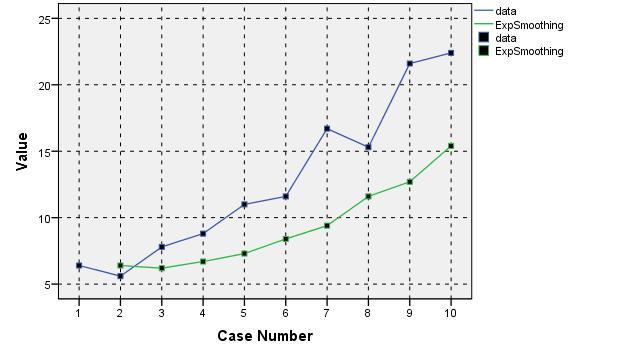
\includegraphics[width=1.00\textwidth]{images/tijdsreeksen/tijdsreeks61.jpg}
	\caption{Exponenti\"ele smoothing bij een trend}
	\label{fig:tijdreeks61}
\end{figure}

Daarom voegen we een extra constante toe om deze trap te overbruggen:

\begin{definition}[Holt-voorspelling of dubbele exponenti\"ele voorspelling]
\begin{eqnarray}
	X_{t} = \alpha x_{t} + (1-\alpha)(X_{t-1} + b_{t-1}) & 0 \leq \alpha \leq 1 \\
	b_{t} = \gamma(X_{t}-X_{t-1}) + (1-\gamma)b_{t-1} & 0 \leq \gamma \leq 1 
\label{eq:doubleSmoothing}
\end{eqnarray}
\end{definition}

\subsubsection{Initi\"ele waarde}
Net zoals in enkelvoudige smoothing kan je verschillende methodes kiezen om initi\"ele waardes voor $X_{t}$ en $b_{t}$ te kiezen:
\begin{itemize}
	\item $X_{1} = x_{1}$
	\item $b_{1} = x_{2} - x_{1}$
	\item $b_{1} = \frac{1}{3}\left[ (x_{2} - x_{1}) + (x_{1} - x_{2}) + (x_{4} - x_{3}) \right]$
	\item $b_{1} = \frac{x_{n} - x_{1}}{n-1}$
\end{itemize}

\subsubsection{Voorspelling}
Een voorspelling maken met dubbele exponenti\"ele smoothing gebeurt dan iets anders (noem $F_{t+1}$ de voorspelling voor tijd $T+1$):

\[ F_{t+1} = X_{t} + b_{t} \]
of
\[ F_{t+m} = X_{t} + m b_{t} \]

Als we nu de tekening maken met enkelvoudige smoothing ($\alpha = 0.977$) en dubbele smoothing ($\alpha = 0.3623, \gamma = 1.0, X_{1} = x_{1} = 6.4$ en $b_{1} = \frac{1}{3}\left[ (x_{2} - x_{1}) + (x_{1} - x_{2}) + (x_{4} - x_{3}) \right] = 0.8$ vinden we volgende waarden in tabel \ref{tab:doubleSingle} en figuur \ref{fig:tijdreeks71}:

\begin{table}
\centering
    \begin{tabular}{|llll|}
    \hline
    Data & Enkelvoudige smoothing $X_{t}$ & Double smoothing $X_{t}$ & $F_{t}$ \\
    6.4  & ~                      & 6.4              & ~                             \\
    5.6  & 6.4                    & 6.6              & 7.2                           \\
    7.8  & 5.6                    & 7.2              & 6.8                           \\
    8.8  & 6.7                    & 8.1              & 7.8                           \\
    11.0 & 8.8                    & 9.8              & 9.1                           \\
    11.6 & 10.9                   & 11.5             & 11.4                          \\
    16.7 & 11.6                   & 14.5             & 13.2                          \\
    15.3 & 16.6                   & 16.7             & 17.4                          \\
    21.6 & 15.3                   & 19.9             & 18.9                          \\
    22.4 & 21.5                   & 22.8             & 23.1                          \\ \hline
    \end{tabular}
		\caption{Tabel met enkelvoudige en dubbele smoothing}
		\label{tab:doubleSingle}
\end{table}

\begin{figure}
	\centering
		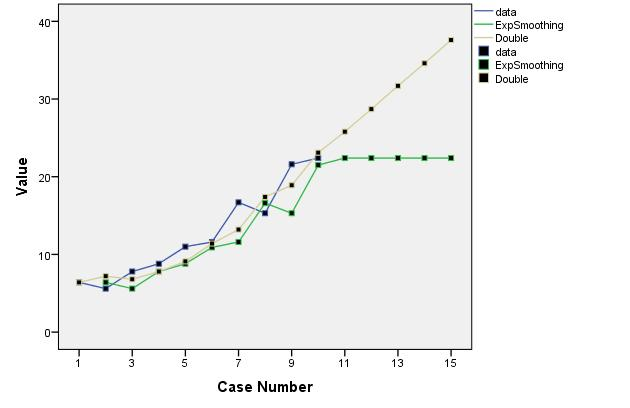
\includegraphics[width=1.00\textwidth]{images/tijdsreeksen/tijdsreeks71.jpg}
	\caption{Enkelvoudige en dubbele smoothing}
	\label{fig:tijdreeks71}
\end{figure}

De manier om dit met R op te lossen is gelijkaardig als bij exponenti\"ele smoothing, alleen moet de parameter gamma $\gamma$ niet op NULL gezet worden. Het maken van de correlogram, de Ljung–Box test en het testen van de normaliteit van de errors gebeurt om dezelfde manier. 

\subsection{Driedubbele exponenti\"ele smoothing}
Wanneer dubbele smoothing niet werkt kan driedubbele smoothing gebruikt worden, ofwel Holt-Winters methode genoemd.

\begin{eqnarray}
	X_{t} = \alpha \frac{x_{t}}{c_{t-L}} + (1-\alpha) (X_{t-1} + b_{t-1}) & \textnormal{Smoothing}\\
	b_{t} = \gamma (X_{t} - X_{t-1}) + (1-\gamma)b_{t-1} & \textnormal{Trend smoothing} \\
	c_{t} = \beta \frac{x_{t}}{X_{t}} + (1-\beta)c_{t-L} & \textnormal{Seasonal smoothing} \\
	F_{t+m} = (X_{t} + mb_{t})c_{t-L+m \mod L}  & \textnormal{Voorspelling}
\label{eq:HoltWinters}
\end{eqnarray}
 met 
\begin{itemize}
	\item $x_{t}$ de observatie op tijdstip $t$
	\item $X_{t}$ is de smoothed observatie op tijdstip $t$
	\item $b_{t}$ is de trendfactor op tijdstip $t$
	\item $c_{t}$ is de seizoensindex op tijdstip $t$
	\item $F_{t}$ is de voorspelling op tijdstip $t$
	\item $L$ is de periode (bv. van de seizoenen)
\end{itemize}

$\alpha, \beta, \gamma$ zijn constanten die geschat moeten worden. 
De manier om dit met R op te lossen is gelijkaardig als bij exponenti\"ele smoothing. Het maken van de correlogram, de Ljung–Box test en het testen van de normaliteit van de errors gebeurt om dezelfde manier. 

\section{Oefeningen}
\label{sec:tijdreeksen-oefeningen}

\begin{exercise}
In bijgevoegd bestand \emph{Budget.csv} vind je vanaf 1981 tot 2005 per kwartaal de omzet, het advertentiebudget en het BNP van een middelgroot bedrijf. Voeg zelf nog een kolom 'Kwartaalnummer' toe.
\begin{enumerate}
	\item Bereken het voortschrijdend gemiddelde \emph{(simple moving average)} over de periodes 4 en 12 voor deze data. Gebruik hiervoor de methode SMA. Maak een lijngrafiek van $X$, $SMA(4)$ en $SMA(12)$.
	\item Welke techniek die we eerder gezien hebben (in het deel over beschrijvende statistiek) is ook geschikt om voorspellingen te maken over de waarden van $X$? Werk dit uit aan de hand van de daarvoor bestemde functie en plot het resultaat in de grafiek.
	\item Gebruik de methode \emph{forecast} om voorspellingen voor de 10 volgende periodes met elk van voorgaande methoden (dus moving average 4 en 10 en regressie) te maken. Teken deze eveneens op de grafiek.
\item Is het gebruik van één van deze technieken interessant om voor deze data voorspellingen te maken? 
\item Maak van de data een tijdreeks via de methode \emph{ts}. Gebruik de methode \emph{decompose} om de tijdreeks op te delen en zo een idee te krijgen van de trend en de seizoenschommeling.
 \item Bereken het exponentieel voortschrijdend gemiddelde \emph{(exponential moving average, EMA)} door gebruik te maken van de methode \emph{HoltWinters}. Maak opnieuw via de methode \emph{forecast} een voorspelling voor 20 periodes. Gebruik als startwaarden $s_1 = x_1$ en $\alpha $ de door R gegenereerde waarde. Plot het resultaat op een nieuwe grafiek samen met $X$.
\item Doe nu hetzelfde met $\alpha=0.1$. 
\item Hoe zien de voorspellingen er nu uit?
\item Doe nu hetzelfde met \emph{dubbele} exponentiële afvlakking. Gebruik als startwaarden $s_1 = x_1$ en $b_1 = \frac{x_n - x_1}{n - 1}$, $\alpha =  0.05$ en $\beta = 0.2$. Plot het resultaat op de grafiek.
\item Gebruik dubbele exponentiële afvlakking om voorspellingen te berekenen voor 20 periodes. Plot de waarden op de grafiek. Is deze techniek beter of slechter dan de vorige voor deze dataset?
\item Speel met de waarden voor $\alpha$ en $\beta$ en bekijk het resultaat, zowel voor enkele als dubbele exponentiële afvlakking.
	\item Gebruik de \emph{HoltWinters}-methode zonder trend.  M.a.w. we stellen $\beta=0$. Gebruik als startwaarden $\alpha =  0.05$ en $\gamma = 0.9$. Plot het resultaat op de grafiek.
\item Bereken opnieuw voorspellingen voor 20 periodes. Plot de waarden op de grafiek. Is deze techniek beter of slechter dan de vorige voor deze dataset?
\item Speel met de waarden voor $\alpha$, $\beta$ en $\gamma$ en bekijk het resultaat.
	\item Gebruik de \emph{HoltWinters}-methode met de door R-gegeneerde waarden zonder trend.  M.a.w. we stellen $\beta=0$.  Plot het resultaat op de grafiek.
\item Bereken opnieuw voorspellingen voor 20 periodes maar gebruik nu de methode \emph{predict}. Plot de waarden op de grafiek. Is deze techniek beter of slechter dan de vorige voor deze dataset?
\end{enumerate}	
	
\end{exercise}

\begin{exercise}
	In bestand \emph{Passagiers2.csv} vind je vanaf januari 1949 tot december 1960 het aantal passagiers van een luchtvaartmaatschappij. 
	\begin{enumerate}
		\item Bereken het voortschrijdend gemiddelde \emph{(simple moving average)} over de periodes 4 en 12 voor deze data. Gebruik hiervoor de methode \emph{ma}. Maak een lijngrafiek van $X$, $MA(4)$ en $MA(12)$.
		\item Welke techniek die we eerder gezien hebben (in het deel over beschrijvende statistiek) is ook geschikt om voorspellingen te maken over de waarden van $X$? Werk dit uit aan de hand van de daarvoor bestemde functie en plot het resultaat in de grafiek.
		\item Gebruik de methode \emph{forecast} om voorspellingen voor de 10 volgende periodes met elk van voorgaande methoden (dus moving average 4 en 10 en regressie) te maken. Teken deze eveneens op de grafiek. Conclusie?
			\item Is het gebruik van één van deze technieken interessant om voor deze data voorspellingen te maken? 
		\item Gebruik de methode \emph{decompose} om de tijdreeks op te delen en zo een idee te krijgen van de trend en de seizoenschommeling.
			\item Bereken het exponentieel voortschrijdend gemiddelde \emph{(exponential moving average, EMA)} door gebruik te maken van de methode \emph{ses} met $\alpha=0.2$. Maak opnieuw via de methode \emph{forecast} een voorspelling voor 20 periodes. Plot het resultaat op een nieuwe grafiek samen met $X$.
		\item Doe nu hetzelfde met $\alpha=0.6$ en $\alpha=0.89$. 
		\item Hoe zien de voorspellingen er nu uit?
			\item Doe nu hetzelfde met \emph{dubbele} exponentiële afvlakking. Gebruik hiervoor de methode \emph{holt}  $\alpha =  0.8$ en $\beta = 0.2$. Plot het resultaat op de grafiek.
		\item Gebruik dubbele exponentiële afvlakking om voorspellingen te berekenen voor 20 periodes. Plot de waarden op de grafiek. Is deze techniek beter of slechter dan de vorige voor deze dataset?
		\item Gebruik in de methode de optie $exponential=TRUE$. Teken het resultaat.  Wat is het verschil?
			\item Gebruik de \emph{hw}-methode met de door R gegeneerde waarden. Plot het resultaat op de grafiek.
		\item Bereken opnieuw een aantal voorspellingen via de methode \emph{predict}. Plot de waarden op de grafiek. Is deze techniek beter of slechter dan de vorige voor deze dataset?
		\item Speel met de waarden voor $\alpha$, $\beta$ en $\gamma$ en bekijk het resultaat.
	\end{enumerate}
	
\end{exercise}	

\begin{exercise}
	
\end{exercise}

\begin{appendices}
\chapter{Logistisch regressie}

\section{Inleiding}

In dit onderzoek gaan we een andere vorm van verband zoeken tussen variabelen waarbij de afhankelijke variabele twee waarden kan aannemen. 

\begin{example}
	\label{ex:slagen}
	Stel dat je wil nagaan of het student al dan niet zal slagen voor het examen onderzoekstechnieken. We zijn dus ge\"interesseerd in de voorspelling (door
	onafhankelijke variabelen) van de kans dat een student in de categorie 'examen slagen' of in de categorie 'niet slagen' valt. 
\end{example}

In bovenstaand voorbeeld zal een 'gewone' lineaire regressie analyse 
algemeen wel de juiste richting van de $\beta$-co\"efficiënten opleveren. Maar de schatting is niet helemaal correct, omdat enkele belangrijke regressie assumpties geschonden worden, zoals de normaliteitsassumptie en de assumptie van homoscedasticiteit. Het grootste probleem is evenwel dat de door lineaire regressie voorspelde kansen groter kunnen zijn dan 1 en kleiner dan 0 en dat is niet te interpreteren.

Bij logistische regressie gaan we werken met kansverhoudingen. In voorbeeld \ref{ex:slagen} hebben we een kansverdeling dat een student wel slaagt $p$ gedeeld door de kans om niet te slagen $1-p$:
\[ 
	\textnormal{verhouding} = \frac{p}{1-p}
\]

We wensen dat de waarden van de verhouding gaan van $- \infty$ tot $\infty$ gaan. Daarom gaan we de natuurlijke logaritme nemen van de verhouding. Om de functie te tekenen van de logaritmische functie kan je onderstaande code gebruiken. 

\lstinputlisting{data/logcurve.R}

Als we de onafhankelijke variabelen $X_1$, $X_2$  \dots $X_n$ noemen,dan ziet het logistische model er in formulevorm als volgt uit:
\[ 
	log(\frac{p}{1-p}) = \beta_0 + \beta_1 X_1 + \cdots + \beta_n X_n 
\]

We kunnen het kansmodel ook herschrijven (afzonderen van de p):

\[ 
	p = \frac{e^{\beta_0 + \beta_1 X_1 + \cdots + \beta_n X_n }}{1+ e^{\beta_0 + \beta_1 X_1 + \cdots + \beta_n X_n }}
\]

We kunnen het kansmodel dan ook herschrijven (afzonderen van de $(1-p)$):
\[ 
1-p = \frac{1}{1+ e^{\beta_0 + \beta_1 X_1 + \cdots + \beta_n X_n }}
\]
Aan deze formules is af te lezen dat de kansen $p$ en $1-p$ bij elkaar opgeteld gelijk zijn aan \'e\'en.
Verder is te zien dat de kansen $p$ en $1-p$ afhankelijk zijn van de variabelen $X_1, X_2 \cdots X_n$, maar dat deze afhankelijkheid niet lineair is. Een logistische regressielijn ziet er dus niet als een rechte lijn
uit, maar als een S-vormige curve. (TODO: hier zou een tekening moeten komen van de sigmo\"ide functie).

Bij logistische regressie gaan we dus op zoek naar goede waarden voor $\beta_0 \cdots \beta_n$. Dit kan in R makkelijk door de methode \texttt{glm}.

\section{Logistische regressie in R}

We gaan het voorbeeld nemen dan in Kaggle \footnote{\href{https://www.kaggle.com/c/titanic/data}{https://www.kaggle.com/c/titanic/data}} gegeven wordt. Het bevat de informatie rond de mensen die de reis van de titanic ondernomen hebben en het overleefd hebben of niet. De analyse komt uit het blog artikel \cite{michy}

\subsection{Data cleaning}

We gaan de data opruimen en kijken welke parameters er in het model kunnen zitten. We gaan dit na door te kijken welke parameters in de dataset niet voldoende aanwezig zijn. 

\begin{lstlisting}
sapply(train,function(x) sum(is.na(x)))
sapply(train, function(x) length(unique(x)))
missmap(train, main = "Missing values vs observed")
\end{lstlisting}
Hierbij zien we dat de variabelen \texttt{cabin} te weinig waarden bevat. Ook \texttt{tickets} laten we vallen aangezien dit weinig invloed zal hebben. 
 We nemen dus een subset van de data en gaan hiermee aan de slag. 
 
 


\chapter{Notatie}
\label{app:notatie}

\begin{table}
  \centering
  \begin{tabular}{p{.25\textwidth}p{.75\textwidth}}
    \toprule
    \textbf{Notatie} & \textbf{Betekenis} \\
    \midrule
    $X$                       & Een stochastische variabele \\
    $N$                       & De populatieomvang \\
    $n$                       & De steekproefgrootte \\
    $\mu$ (mu)                & Het gemiddelde (ook: verwachtingswaarde) over heel de \emph{populatie}. \\
    $\overline{x}$            & Het gemiddelde over de \emph{steekproef} \\
    $\sigma$ (sigma)          & De standaardafwijking over heel de populatie \\
    $s$                       & De standaardafwijking over de steekproef \\
    $X \sim Nor(\mu, \sigma)$ & De variabele $X$ is \emph{normaal verdeeld} met gemiddelde $\mu$ en standaardafwijking $\sigma$ \\
    $Z \sim Nor(0, 1)$        & $Z$ is een variabele met een kansverdeling die de \emph{standaardnormaalverdeling} volgt, dus met gemiddelde 0 en standaardafwijking 1 \\
    $M$                       & De kansverdeling van het populatiegemiddelde, op basis van een steekproef (cfr.~de centrale limietstelling, Sectie~\ref{sec:centrale-limietstelling}) \\

    \bottomrule
  \end{tabular}
\end{table}


\clearpage
\addcontentsline{toc}{chapter}{\textcolor{maincolor}{\IfLanguageName{dutch}{Bibliografie}{Bibliography}}}
\printbibliography

\clearpage
\addcontentsline{toc}{chapter}{\textcolor{maincolor}{Index}}
\printindex
\end{appendices}
\end{document}
